\documentclass[]{book}
\usepackage{lmodern}
\usepackage{amssymb,amsmath}
\usepackage{ifxetex,ifluatex}
\usepackage{fixltx2e} % provides \textsubscript
\ifnum 0\ifxetex 1\fi\ifluatex 1\fi=0 % if pdftex
  \usepackage[T1]{fontenc}
  \usepackage[utf8]{inputenc}
\else % if luatex or xelatex
  \ifxetex
    \usepackage{mathspec}
  \else
    \usepackage{fontspec}
  \fi
  \defaultfontfeatures{Ligatures=TeX,Scale=MatchLowercase}
\fi
% use upquote if available, for straight quotes in verbatim environments
\IfFileExists{upquote.sty}{\usepackage{upquote}}{}
% use microtype if available
\IfFileExists{microtype.sty}{%
\usepackage{microtype}
\UseMicrotypeSet[protrusion]{basicmath} % disable protrusion for tt fonts
}{}
\usepackage[margin=1in]{geometry}
\usepackage{hyperref}
\hypersetup{unicode=true,
            pdftitle={The Anatomy Of Negation},
            pdfauthor={Edgar Saltus},
            pdfborder={0 0 0},
            breaklinks=true}
\urlstyle{same}  % don't use monospace font for urls
\usepackage{natbib}
\bibliographystyle{apalike}
\usepackage{longtable,booktabs}
\usepackage{graphicx,grffile}
\makeatletter
\def\maxwidth{\ifdim\Gin@nat@width>\linewidth\linewidth\else\Gin@nat@width\fi}
\def\maxheight{\ifdim\Gin@nat@height>\textheight\textheight\else\Gin@nat@height\fi}
\makeatother
% Scale images if necessary, so that they will not overflow the page
% margins by default, and it is still possible to overwrite the defaults
% using explicit options in \includegraphics[width, height, ...]{}
\setkeys{Gin}{width=\maxwidth,height=\maxheight,keepaspectratio}
\IfFileExists{parskip.sty}{%
\usepackage{parskip}
}{% else
\setlength{\parindent}{0pt}
\setlength{\parskip}{6pt plus 2pt minus 1pt}
}
\setlength{\emergencystretch}{3em}  % prevent overfull lines
\providecommand{\tightlist}{%
  \setlength{\itemsep}{0pt}\setlength{\parskip}{0pt}}
\setcounter{secnumdepth}{5}
% Redefines (sub)paragraphs to behave more like sections
\ifx\paragraph\undefined\else
\let\oldparagraph\paragraph
\renewcommand{\paragraph}[1]{\oldparagraph{#1}\mbox{}}
\fi
\ifx\subparagraph\undefined\else
\let\oldsubparagraph\subparagraph
\renewcommand{\subparagraph}[1]{\oldsubparagraph{#1}\mbox{}}
\fi

%%% Use protect on footnotes to avoid problems with footnotes in titles
\let\rmarkdownfootnote\footnote%
\def\footnote{\protect\rmarkdownfootnote}

%%% Change title format to be more compact
\usepackage{titling}

% Create subtitle command for use in maketitle
\newcommand{\subtitle}[1]{
  \posttitle{
    \begin{center}\large#1\end{center}
    }
}

\setlength{\droptitle}{-2em}

  \title{The Anatomy Of Negation}
    \pretitle{\vspace{\droptitle}\centering\huge}
  \posttitle{\par}
    \author{Edgar Saltus}
    \preauthor{\centering\large\emph}
  \postauthor{\par}
    \date{}
    \predate{}\postdate{}
  
\usepackage{booktabs}
\usepackage{amsthm}
\makeatletter
\def\thm@space@setup{%
  \thm@preskip=8pt plus 2pt minus 4pt
  \thm@postskip=\thm@preskip
}
\makeatother

\begin{document}
\maketitle

{
\setcounter{tocdepth}{1}
\tableofcontents
}
\chapter*{The Anatomy Of Negation}\label{the-anatomy-of-negation}
\addcontentsline{toc}{chapter}{The Anatomy Of Negation}

\begin{figure}
\centering
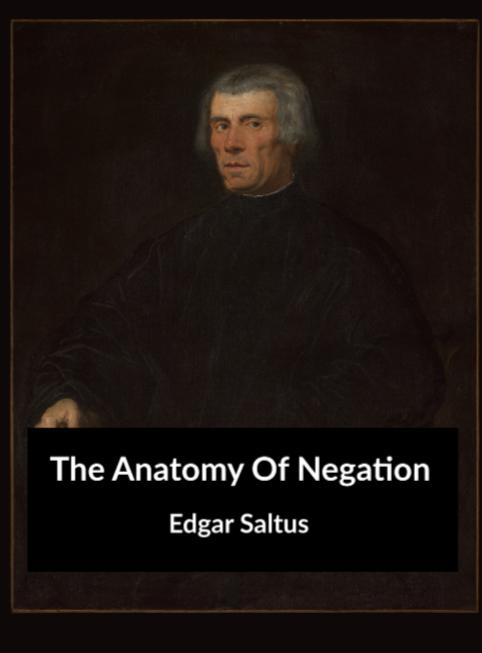
\includegraphics{./assets/h.jpg}
\caption{}
\end{figure}

\begin{quote}
Quoy qu'on nous presche, il fauldroit toujours se souvenir que c'est
I'honime qui donne et l'homme qui reçoit.
\end{quote}

\begin{itemize}
\tightlist
\item
  Montaigne
\end{itemize}

\begin{quote}
II est un jour, une heure, où dans le chemin rude, Courbé sous le
fardeau des ans multipliés, L'Esprit humain s'arrête, et pris de
lassitude, Se retourne pensif vers les jours oubliés.
\end{quote}

\begin{quote}
La vie a fatigué son attente inféconde; Désabusé du Dieu qui ne doit
point venir, II sent renaître en lui la jeunesse du monde; II écoute ta
voix, ô sacré souvenir!
\end{quote}

\begin{quote}
Mais si rien ne répond dans l'immense étendue Que le stérile écho de
l'éternel désir, Adieu, déserts, ou l'âme ouvre une aile éperdue! Adieu,
songe sublime, impossible à saisir.
\end{quote}

\begin{quote}
Et toi, divine Mort, où tout rentre et s'efface, Accueille tes enfants
dans ton sein étoilé; Affranchis-nous du temps, du nombre et de
I'espace, Et rends-nous le repos que la vie a troublé.
\end{quote}

\begin{itemize}
\tightlist
\item
  Leconte de Lisle
\end{itemize}

\textbf{Prefatory Note}

The accompanying pages are intended to convey a tableau of anti-theism
from Kapila to Leconte de Lisle. The anti-theistic tendencies of England
and America have been treated by other writers; in the present volume,
therefore, that branch of the subject is not discussed. To avoid
misconception, it may be added that no attempt has been made to prove
anything.

\begin{itemize}
\tightlist
\item
  Biarritz, 15th September, 1886.
\end{itemize}

\chapter{The Revolt Of the Orient}\label{the-revolt-of-the-orient}

Man, as described by Quatrefages, is a religious animal. The early
naturalists said the same thing of the elephant; but while this
statement, which contains all the elements of a libel, has fallen into
disrepute, the former, little by little, has assumed the purple among
accepted facts.

Man's belief in the supernatural antedates chronology. It was unfathered
and without a mother. It was spontaneous, natural, and unassisted by
revelation. It sprang into being with the first flight of fancy.

The characteristic trait of primitive man seems to have been that of
intellectual passivity. He was never astonished: if he noticed anything,
it was his own weakness the power of the elements he accepted as a
matter of course. The phenomena that he witnessed, the sufferings that
he endured, were to him living enemies whose violence could be conjured
by prayers and donations. Everything had its spectre; phantoms were as
common as leaves. There was not a corner of the earth unpeopled by
vindictive demons. In sleep he was visited by them all, and as his
dreams were mainly nightmares, his dominant sensation was that of
fright.

As his mind developed, frontiers were outlined between the imaginary and
the real; the animate and the inanimate ceased to be identical. Instead
of attributing a particular spirit to every object, advancing theology
conceived a number of aggrandised forces. The earth, sea and sky were
laid under contribution, and the phenomena of nature were timidly
adored. In the course of time these open-air deities were found smitten
by a grave defect - they were visible. The fear of the unseen demanded
something more mysterious, a hierarchy of invisible divinities of whom
much might be suspected and but little known. It was presumably at this
point that the highroad to polytheism was discovered; and when man grew
to believe that the phenomena which his ancestors had worshipped were
but the unconscious agents of higher powers, the gods were born.

Consecutive stages of development such as these have evidently been far
from universal. There are races whose belief in the supernatural is so
accidental that any classification is impossible. There are others in
whose creeds the transition from animism to broader views is still
unmarked. In the equatorial regions of Africa, in Madagascar, Polynesia,
and among certain Tartar tribes, animism and its attendant fetishism is
reported to be still observable. The distinction between the palpable
and the impalpable, the separation between what is known to be material
and that which is conceived to be divine, does not necessarily exist
even in countries that have reached a high degree of civilisation. In
India, the dance of the bayaderes before the gilded statues, and the
top-playing that is to amuse a stone Krishna, are cases in point. But
these instances are exceptions to the general rule. It seems well
established that man, in proportion to his intelligence, passed out of
animism, loitered in polytheism, and drifted therefrom into monotheistic
or pantheistic beliefs.

The race whose beliefs have held most steadfast from their incipiency to
the present day is the Hindu. In their long journey these beliefs have
encountered many vicissitudes; they have been curtailed, elaborated and
degraded, but in the main they are still intact. At the contact with
fresher faiths, the primitive religions of other lands have either
disappeared abruptly or gradually faded away. It is India alone that has
witnessed an autonomous development of first theories, and it is in
India that the first denying voice was raised. To appreciate the denial
it is necessary to understand what was affirmed. For this purpose a
momentary digression may be permitted.

In the beginning of the Vedic period, Nature in her entirety was held
divine. To the delicate imagination of the early Aryan, the gods were in
all things, and all things were gods. In no other land have myths been
more fluid and transparent Mountains, rivers and landscapes were
regarded with veneration; the skies, the stars, the sun, the dawn and
dusk were adored, but particularly Agni, the personification of creative
heat. Through lapse of time of which there is no chronology, this
charming naturalism drifted down the currents of thought into the
serenest forms of pantheistic beliefs.

The restless and undetermined divinities, omnipresent and yet
impalpable, the wayward and changing phenomena, contributed one and all
to suggest the idea of a continuous transformation, and with it, by
implication something that is transformed. Gradually the early
conception of Agni expanded into a broader thought. From the spectacle
of fire arose the theory of a deva, one who shines; and to this deva a
name was given which signified both a suppliant and a supplication -
Brahma. In this metamorphosis all vagueness was lost. Brahma became not
only a substantial reality, but the creator of all that is. Later, the
labour of producing and creating was regarded as an imperfection, a
blemish on the splendour of the Supreme. It was thought a part of his
dignity to be majestically inert, and above him was conceived the
existence of a still higher being, a being who was also called Brahma;
yet this time the name was no longer masculine, but neuter - and
indeclinable neuter as having no part in life, and indeclinable because
unique. \footnote{Essai sur le Veda. Taine: Essais}

This conception of a neuter principle, eternal, inactive, and a trifle
pale perhaps, was not reached during the period assigned to the Vedas.
It was the work of time and of fancy, but it was unassisted. The
religion of India is strictly its own; its systems were founded and its
problems solved almost before the thinkers of other lands were old
enough to reflect. In Greece, which was then in swaddling clothes,
Anaxagorus was the first who thought of a pure Intelligence, and this
thought he contented himself with stating; its development was left to
other minds, and even then it remained unadorned until Athens heard the
exultant words of Paul. Nor could the Hindus have gathered their ideas
from other countries. Their brothers, the Persians, were watching the
combat between Ahura-Mazda and Ahriman. With the Hebrews there was no
chance nor rumour of contact: Elohim had not given way to Jehovah.
Chaldea was celebrating with delirious rites the nuptials of Nature and
the Sun; while far beyond was Egypt, and on her heart the Sphinx.

It seems, then, not unsafe to say that the Vedas and the theories that
were their aftergrowth have no connection with any foreign.
civilisation. Beyond this particular, Brahmanism enjoys over all other
religions the peculiar distinction of being without a founder. Its germ,
as has been hinted, was in the Vedas; but it was a germ merely that the
priests planted and tended, and watched develop into a great tree, which
they then disfigured with unsightly engraftments.

Emerson recommended us to treat people as though they were real, and
added, ``Perhaps they are.'' But the doubt that lingered in the mind of
the stately pantheist never entered into that of the Hindu. In its
purest manifestation the creed of the latter was a negation of the
actuality of the visible world. The forms of matter were held to be
illusive, and the semblance of reality possessed by them was considered
due to Maya. Maya originally signified Brahma's longing for something
other than himself; something that might contrast with his eternal
quietude; something that should occupy the voids of space; something
that should lull the languors of his infinite ennui. From this longing
sprang whatever is, and it was through Maya, which afterwards became
synonymous with illusion, that a phantom universe surged before the
god's delighted eyes, the mirage of his own desire.

This ghostly world is the semblance of reality in which man dwells:
mountains, rivers, landscapes, the earth itself, the universe and all
humanity, are but the infinite evolutions of his fancy. The ringing
lines that occur in Mr.Swinburne's ``Hertha'' may not improperly be
referred to him:

\begin{quote}
I am that which began;
\end{quote}

\begin{quote}
Out of me the years roll;
\end{quote}

\begin{quote}
Out of me, God and man;
\end{quote}

\begin{quote}
I am equal and whole.
\end{quote}

\begin{quote}
God changes, and man, and the form of them bodily.
\end{quote}

\begin{quote}
I am the soul.
\end{quote}

Familiarly, Brahma is the spider drawing from his breast the threads of
existence; emblematically, a triangle inscribed in a circle; poetically,
the self-existing supremacy that is enthroned on a lotus of azure and
gold; and theologically, the one really existing essence, the eternal
germ from which all things issue and to which all things at last return.

From man to Brahma, a series of higher forms of existence are traceable
in an ascending scale till three principal divinities are reached.
These, the highest manifestations of the First Cause, Brahma the
Creator, Vishnu the Preserver, and Siva the Destroyer, constitute the
Tri-murti, the Trinity, typified in the magically mystic syllable Om. To
these were added a host of inferior deities and even local gods similar
to those which the Romans recognised in later years. Such was and still
is the celestial hierarchy. In the eyes of the Hindu, none of these gods
are eternal. At the end of cycles of incommensurable duration, the
universe will cease to be, the heavens will be rolled up like a garment,
the Tri-murti dissolved; while in space shall rest but the great First
Cause, through whose instrumentality, after indefinite kalpas, life will
be re-beckoned out of chaos and the leash of miseries unloosed.

This delicious commingling of the real and the ideal degenerated with
the years. Like Olympus, it was too fair to last. Brahma, Vishnu and
Siva, once regarded as various manifestations of the primal essence,
became in lapses of time concrete. Female counterparts were found for
them, and the most poetic of the creeds of man was lowered into a
sensuous idolatry. To-day there is nothing, however monstrous or
grotesque, that is deemed unfit for worship. In Benares there is a
shrine to small-pox; in Gaya there is one to the police and it may be
that somewhere between Cape Comorin and the Himalayas an altar has been
raised to those who dull digestion with the after-dinner speech.

This, however, is the work of the priest. In earlier days the higher
castes of man, the younger brothers of the gods, were thought capable of
understanding the perfection that resides in Brahm. It was held that
they might ascend to the rank of their elders, and with them at last be
absorbed in the universal spirit. The one pathway to this goal was
worship, and over it the priests constituted themselves the lawful
guides.

The laws which they codified were numberless, and an infraction of any
one of them was severely visited on the transgressor. For each fault,
whether of omission or commission, there was an expiation to be
undergone, and it was taught that the unatoned violation of a precept
precipitated the offender into one of twenty-eight hells which their
inflammable imaginations had created.

In the face of absurdities such as these, it is permissible to suppose
that, like the Roman augurs, the educated Brahmans could not look at
each other without laughing; yet, however this may be, it seems certain
that many of the laity laughed at them. Already in the Rig-Veda mention
was made of those who jeered at Agni. The question as to whether there
is really another life seems to have been often raised, and that too in
the Brahmanas. Yaska, a venerable sage, found himself obliged to refute
the opinions of sages far older and more venerable than himself, who had
declared the Vedas to be a tissue of nonsense. This scepticism had found
many adherents. The name given to these early disbelievers was Nastikas
- They who deny. Like other sects, they had aphorisms and slokas of
their own, which with quaint derision they attributed to the tutor of
the gods. The aphorisms appear to have been markedly anti-theistic,
while the slokas were captivating invitations to the pleasures of life.

\begin{quote}
Vivons, ouvrons nos coeurs aux ivresses nouvelles:
\end{quote}

\begin{quote}
Dormir et boire en paix, voilà l'unique bien.
\end{quote}

\begin{quote}
Buvons! Notre sang brûle et nos femmes sont belles:
\end{quote}

\begin{quote}
Demain n'est pas encore, et le passé n'est rien!
\end{quote}

Among those who laughed the loudest was Kapila. His life is shrouded in
the dim magnificence of legends. There let it rest; yet if little can be
said of the man, his work at least is not unfamiliar to students. The
Sankhya Karika, which bears his name, is one of the most important and
independent relics of Indian thought. In its broadest sense, Sankhya
means rationalism or system of rational philosophy. In India it is known
as the philosophy Niriswara, the philosophy without a god.

Kapila was the first serious thinker who looked up into the archaic
skies and declared them to be void. In this there was none of the
moderation of scepticism, and less of the fluctuations of doubt. Kapila
saw that the idea of a Supreme Being was posterior to man; that Nature,
anterior to her demiurge, had created him; and he resolutely turned his
back on the Tri-murti, and denied that a deity existed, or that the
existence of one was necessary to the order and management of the world.
The motor-power he held to be a blind, unconscious force, and of this
force life was the melancholy development. If he had disbelieved in
transmigration, Schopenhauer would not have startled the world with a
new theory.

Kapila's purpose was to relieve man from pain. There were no rites to be
observed. Knowledge and meditation were alone required. He recognised
but three things - the soul, matter and pain. Freedom from pain was
obtainable, he taught, by the liberation of the soul from the bondage of
matter. According to his teaching, the heavens, the earth and all that
in them is, are made up of twenty-five principles, and of these
principles matter is the first and the soul the last. Matter is the
primordial element of universal life, the element that animates and
sustains all things. The principles that succeed it are simply its
developments. Of these, the soul is the chief. It is for matter to act
and for the soul to observe. When its observations are perfect and
complete, when it has obtained a discriminative knowledge of the forms
of matter, of primeval matter and of itself, then is it prepared to
enter into eternal beatitude.

On the subject of eternal beatitude, each one of the systems of Eastern
thought has had its say. That which Kapila had in view is not entirely
clear. He gave no description of it otherwise than in hinting that it
was a state of abstract and unconscious impassabiUty, and he appears to
have been much more occupied in devising means by which man might be
delivered from the evils of life than in mapping charts of a fantastic
paradise.

The sentiment of the immedicable misery of life is as prominent in the
preface of history as on its latest and uncompleted page. The problem of
pain agitated the minds of the earliest thinkers as turbulently as it
has those of the latest comers. In attempting to solve it, in
endeavouring to find some rule for a law of error, the Hindu accepted an
unfathered idea that he is expiating the sins of anterior and
unremembered existences, and that he will continue to expiate them until
all past transgressions are absolved and the soul is released from the
chain of its migrations. According to the popular theory, the chain of
migrations consists in twenty-four lakhs of birth, a lakh being one
hundred thousand.

Apparently such beatitude as lay beyond the tomb consisted to Kapila in
relief from transmigration, and this relief was obtainable by the
ransomed soul, only, as has been hinted, through a knowledge acquired of
matter and of itself. Garmented in the flesh of him that constitutes its
individuality, the soul was to apply itself to understanding of Nature,
who, with the coquetry of a bayadere, at first resists and then unveils
her beauties to the eyes of the persistent wooer. This knowledge once
obtained, the soul is free. It may yet linger awhile on earth, as the
wheel of the spinner turns for a moment after the impulse which put it
in motion has ceased to act; but from that time the soul has fulfilled
all the conditions of its deliverance, and is for ever afiranchised from
the successive migrations which the unransomed soul must still undergo.

In his attack on official theology, Kapila paid little attention to its
rites and observances. He probably fancied that if the groundwork was
undermined, the superstructure would soon totter. In this he was
partially correct, though the result of his revolt was entirely
different from what he had expected. The climax of his philosophy is a
metaphysical paradox: ``Neither I am, nor is aught mine, nor is there
any I'' - a climax which must have delighted Hegel, but one which it is
difficult to reconcile with the report of the philosophy's present
popularity. And that it is popular there seems to be no doubt. There is
even a common saying in India that no knowledge is equal to the Sankhya,
and no power equal to the Yoga, which latter, a combination of mnemonics
and gymnastics, is a contrivance for concentrating the mind intently on
nothing.

But whatever popularity the Sankhya may now enjoy, it is evident that,
like other systems of Eastern thought, it was understood only by adepts;
and even had the science which it taught been offered to the people, it
was not of a nature to appeal to them. The masses today are as ignorant
as carps, and at that time they were not a whit more intelligent.
Besides, it was easier to understand the Tri-murti than twenty-five
abstract principles. Brahma was very neighbourly, and his attendant gods
were known to tread the aisles of night. The languid noons and sudden
dawns were sacred with their presence. What could be more reasonable? If
life was an affliction, that very affliction carried the sufferer into
realms of enchantment, where Brahma was enthroned on a lotus of azure
and gold.

It is small wonder then that Kapila's lessons left the established
religion practically unharmed. Kant's ``Kritik'' did not prevent the
Koenigsbergians from listening to the \emph{Pfarrer} with the same faith
with which their fathers had listened before them. And Kant, it may be
remembered, was not only a popular teacher, he was one that was revered.
But aside from any influence that Kapila's philosophy may have exerted,
it was evidently smitten by a grave defect. Concerning the soul's
ultimate abiding-place it was silent. This silence enveloped the entire
system in an obscurity which another and a greater thinker undertook to
dissipate.

It has been said before, and with such wisdom that the saying will bear
repetition, that revolutions are created, not by the strength of an
idea, but by the intensity of a sentiment. In great crises there is a
formula that all await; so soon as it is pronounced, it is accepted and
repeated it is the answer to an universal demand. Toward the close of
the sixth century before the present era, at Kapilavastu, a city and
kingdom situated at the foot of the mountains of Nepal, a prince of the
blood, after prolonged meditations on the misfortunes of life,
pronounced a watchword of this description.

The name of this early Muhammad was Siddartha. He was the heir of the
royal house of Sakya, and in later years, in remembrance of his origin,
he was called Sakya-Muni, Sakya the Anchorite, to which was added the
title of Buddha, the Sage. The accounts of his life are contained in the
Lalita Vistara, a collection of fabulous episodes in which the
supernatural joins hands with the matter-of-fact. It is said, for
instance, that he was born of an immaculate conception, and died of an
indigestion of pork. Apart from the mythical element, his life does not
appear to have been different from that of other religious reformers,
save only that he is supposed to have been born in a palace instead of a
hovel. To his twenty-ninth year Siddartha is represented as living at
court, surrounded by all the barbaric ease and gorgeousness of the Ind.
Yet even in his youth his mind appears to have been haunted by great
thoughts. He took no part in the sports of his companions, and was
accustomed, it is said, to wander away into the solitudes of the vast
forests of bamboo, and there to linger, lost in meditation.

In the course of time he was married to a beautiful girl, but even in
her fair arms his thoughts were occupied with the destinies of the
world. During the succeeding festivals and revels, amid the luxury of
the palace and the enticements of love, he meditated on the miseries of
life. In Brahmanism he found no consolation. At its grotesqueness he too
smiled, but his smile was nearer to tears than to laughter. The
melancholy residue of his reflections was with him even in dream, and
one night - so runs the legend - he was encouraged in a vision to teach
mankind a law which should save the world and establish the foundation
of an eternal and universal rest.

A combination of fortuitous circumstances, the play of the merest
hazard, appear to have strengthened the effect of this vision. On the
high-roads about Kapilavastu he encountered a man bent double with age,
another stricken by fever, and lastly a corpse. ``A curse,'' he cried,
``on youth that age must overcome; a curse on health that illness
destroys; a curse on life which death interrupts! Age, illness, death,
could they but be for ever enchained!'' Soon after, he disappeared, and
seeking the jungles, which at that time were peopled with thinkers of
ken, he devoted himself to the elaboration of his thoughts. It was there
that he seems to have acquired some acquaintance with the philosophy of
Kapila. He divined its significance and saw its insufficiency.
Thereafter for six years he gave himself up to austerities so severe
that, in the naive language of the legend, they startled even the gods.
These six years are said to have been passed at Ouruvilva, a place as
famous in Buddhist annals as Kapilavastu. In this retreat he arranged
the principles of his system, and perfected the laws and ethics which
were to be its accompaniment. Yet still the immutable truth that was to
save the world escaped him. A little longer he waited and struggled. The
Spirit of Sin, with all his seductive cohorts, appeared before him. The
cohorts were routed and the Spirit overcome; the struggle was ended; and
under a Bodhi-tree which is still shown to the pilgrim, Siddartha caught
the immutable truth, and thereupon presented himself as a saviour to his
fellows.

Such is the popular legend. Its main incidents have been recently and
most felicitously conveyed in \emph{The Light of Asia}. As a literary
contribution, Mr.~Arnold's poem is simply charming; as a page of
history, it has the value of a zero from which the formative circle has
been eliminated. The kingdom of Kapilavastu, or rather Kapilavatthu, was
an insignificant hamlet. The Buddha's father was a petty chieftain, the
raja of a handful of ignorant savages. Palaces he had none; his wealth
was his strength; and could his concubine be recalled to Hfe, she would,
had she any sense of humour, which is doubtful, be vastly amused at
finding that she had been given a role in the solar myth.

There can, however, be no doubt that the Buddha really lived. His
existence is as well established as that of the Christ. To precisely
what an extent he was a visionary is necessarily difficult of
conjecture. Yet unless all beHef in him be refused, it seems almost
obligatory to assume that after years of reflection he considered
himself in possession of absolute knowledge. The truth which he then
began to preach was not a doctrine that he held as personal and peculiar
to himself, but rather an eternal and changeless law which had been
proclaimed from age to age by other Buddhas, of whom he fancied himself
the successor.

To speak comparatively, it is only with recent years that the attention
of Western students has been attracted to Buddhist literature. Today,
however, thanks to translations from the Pali and kindred tongues, it is
possible for any one to study the doctrine from the sacred books
themselves.

There are verses in the Vedas which when recited are said to charm the
birds and beasts. Compared with them, the Buddhist Gospels are often
lacking in beauty. To be the better understood, the priests, who
addressed themselves not to initiates but to the masses, employed a
language that was simple and familiar. There are in consequence many
repetitions and trivial digressions, but there are also parables of such
exquisite colour, that in them one may feel the influence of a bluer sky
than ours, the odour of groves of sandal, the green abysses of the
Himalayas, and the gem-like splendour of white Thibetian stars.

The Buddha believed neither in a personal nor an impersonal God. The
world he compared to a wheel turning ceaselessly on itself. Of Brahman
tenets he preserved but one, that of the immedicable misery of life. But
the doctrine which he taught may perhaps best be summarised Bs resting
on three great principles - Karma, Arahatship and Nirvana. When these
principles are understood, the mysteries of the creed are dissolved, and
the need of esoteric teaching diminished.

It may be noted, by way of proem, that the theory of the transmigration
of souls is not advanced in the Vedas. It is a part of Brahman teaching,
but Brahmanism and Vedaism are not the same. The Vedas are claimed as
the outcome of direct revelation, while all that part of post-Vedic
literature in which Brahmanism is. enveloped is held to be purely
traditional The origin of the theory of the transmigration is
indiscoverable, but it is one which has been shared by many apparently
unrelated races. It was a part of the creed of the Druids; the
Australian savage, as well as some of the American aborigines, held to
the same idea; thinkers in Egypt and in Greece advanced identical
tenets; it is alluded to in the Talmud, and hinted at in the Gospel
which bears the name of St.~John. Possibly it was held by the pre-Aryan
inhabitants of India, and in that case it is equally possible that it
was through them that the doctrine descended into Brahmanism. But
whether or not its engraftment came about in this way is relatively a
matter of small moment. The important point to be observed is that it
was not received by the Buddhists. The popular idea to the contrary is
erroneous.

Spinoza noted that there is in every man a feeling that he has been what
he is from all eternity, and this feeling has not left the Buddhist
unaffected. But between such a sentiment and a belief in transmigration
the margin is wide. The popular error in which the two are confused has
presumably arisen from a misunderstanding of the laws of Karma and
Vipaka, the laws of cause and effect. The difference therein
discoverable amounts in brief to this in the theory: of transmigration
the soul is held to be eternal in Buddhism the existence of the soul is
denied. In the one, the ego resurrects through cycles of unremembered
lives; in the other, nothing survives save the fruit of its actions. In
the one, every man is his own heir and his own ancestor in the other,
the deeds of the ancestor are concentrated in a new individual. In each
there is a chain of existences, but in the one they are material, in the
other they are moral. One maintains the migration of an essence, the
other the results of causality; one has no evidence to support it, the
other accords with the law of the indestructibihty of force. One is
metempsychosis, the other palingenesis; one is beautiful, and the other
awkward; but one is merely a theory, and the other is almost a fact.

From this chain the Hindu knew no mode of relief. Prior to the Buddha's
advent, there was an unquestioned belief that man and all that
encompasses him rolled through an eternal circle of transformation; that
he passed through all the forms of life, from the most elementary to the
most perfect; that the place which he occupied depended on his merits or
demerits; that the virtuous revived in a divine sphere, while the wicked
descended to a yet darker purgatory; that the recompense of the blessed
and the punishment of the damned were of a duration which was limited;
that time effaced the merit of virtue as well as the demerit of sin; and
that the law of transmigration brought back again to earth both the just
and the unjust, and threw them anew into a fresh cycle of terrestrial
existences, from which they could fight free as best they might.

When the Buddha began to teach, he endeavoured to bring his new theories
into harmony with old doctrines. Throughout life, man, he taught, is
enmeshed in a web whose woof was woven in preceding ages. The
misfortunes that he endures are not the consequences of his immediate
actions; they are drafts which have been drawn upon him in earlier days
- drafts which he still must honour, and against which he can plead no
statute of limitations. Karma pursues him in this life, and unless he
learns its relentless code by heart, the fruit of his years is caught up
by revolving chains, and tossed back into the hfe of another. How this
occurred, or why it occurred, is explainable only by a cumbersome
process from which the reader may well be spared; and it may for the
moment suffice to note that while the Buddha agreed with the Brahmans
that life formed a chain of existences, it was the former who brought
the hope that the chain might be severed.

The means to the accomplishment of this end consist in a victory over
the lusts of the flesh, the desire for life and the veils of illusion.
When these have been vanquished, the Arahat, the victor, attains
Nirvana.

Nirvana, or Nibbana as it stands in the Pali, is not a paradise, nor yet
a state of post-mortem trance. It is the extinction of all desire, the
triple victory of the Arahat, which precedes the great goal, eternal
death. The fruit of earlier sins remain, but they are impermanent and
soon pass away. Nothing is left from which another sentient being can be
called into existence. The Arahat no longer lives; he has reached Para
Nirvana, the complete absence of anything, that can be likened only to
the flame of a lamp which a gust of wind has extinguished.

The Buddha wrote nothing. It was his disciples who, in councils that
occurred after his death, collected and arranged the lessons of their
master. In these synods the canon of sacred scripture was determined. It
consisted of three divisions, called the Tri-pitaka, or Three Baskets,
and contained the Suttas, the discourses of the Buddha - the Dharmas,
the duties enjoined on the masses - and lastly the Vinayas, the rules of
discipline.

The Dharmas contain the four truths whose discovery is credited to the
Buddha. The first is that suffering is the concomitant of life. The
second, that suffering is the resultant of desire. The third, that
Telief from suffering is obtained in the suppression of desire. And
fourth, that Nirvana, which succeeds the suppression of desire, is
attainable only through certain paths. These paths are eight in number;
four of which - correctness in deed, word, thought and sight - were
recommended to all men; the remainder - the paths of application,
memory, meditation and proper life - are reserved for the eremites.

For the use of the faithful, the four truths have been condensed in a
phrase ``Abstain from sin, practise virtue, dominate the flesh - such is
the law of the Buddha.'' The recognition of the four truths and the
observance of the eight virtues are obligatory to all who wish to reach
Nirvana. The neophyte renounces the world and lives a mendicant. Yet
inasmuch as a society of saints is difficult to perpetuate, members are
admitted from whom the usual vows of continence and poverty are not
exacted.

The charm of primitive Buddhism was in its simplicity. The faithful
assembled for meditation and not for parade. The practice of morality
needed no forms and fewer ceremonies. But with time it was thought well
to make some concession to popular superstitions; and although the
Buddha had no idea of representing himself as a divinity, every moral
and physical perfection was attributed to him. The rest was easy.
Idolatry had begun. To the right and left of a saint elevated to the
rank of God Supreme, a glowing Pantheon was formed of the Buddhas that
had preceded him. A meaningless worship was established; virtues were
subordinated to ceremonies; and today before a gilded statue a wheel of
prayers is turned, while through the dim temples, domed like a vase, the
initiates murmur, ``Life is evil.''

In attempting to convert the multitude, the Buddha made no use of vulgar
seductions. From him came no flattery to the passions. The recompense
that he promised was not of the earth nor material in its nature. To his
believers he offered neither wealth nor power. The psychic force, the
seemingly supernatural faculties, that knowledge and virtue brought to
those who had reached superior degrees of sanctity, were shared by the
Brahmans as well; they were an appanage, not a bait. The one reward of
untiring efforts was an eternal ransom from the successive horrors of
Karma. The paradise which he disclosed was the death of Death. In it all
things ceased to be. It was the ultimate annihilation from which life
was never to be re-beckoned.

It is not surprising that the captivating quiet of a goal such as this
should forcibly appeal to the inclinations of the ascetic; the wonder of
it is that it could be regarded for a moment as attractive to the coarse
appetites of the crowd. Nor does it seem that the Christ of Chaos made
this mistake. It was the after-comers who undertook to lift the
commonplace out of the humdrum. The Buddha's hope of the salvation of
all mankind was a dream extending into the indefinite future; the theory
of immediate emancipation was never shared by him. For the plain man, he
laid down a law which was a law of grace for all, that of universal
brotherhood. If its practice was insufficient to lead him to Nirvana, it
was still a preparation thereto, a paving of the way for the travellers
that were yet to come.

The method which he employed to convert his hearers seems to have been a
tender persuasion, in which there was no trace of the dogmatic. He did
not contend against strength, he appealed to weakness, varying the
insinuations of his parables according to the nature of the listener,
and charming even the recalcitrant by the simplicity and flavour of his
words. In these lessons there were no warnings, no detached
maledictions; but there were exhortations to virtue, and pictures of the
sweet and sudden silence of eternal rest. His struggle was never with
creeds, but with man, with the flesh and its appetites; and from the
memory of his victorious combat with himself there came to him precepts
and maxims of incomparable delicacy and beauty. These were his weapons.
His teaching was a lesson of infinite tenderness and compassion; it was
a lesson of patience and resignation and abnegation of self, and
especially of humility, which in its renouncement of temporal splendours
opens the path to the magnificence of death.

In the ears of not a few modern thinkers, this promise of annihilation
has sounded like a gigantic paradox. It has seemed inconceivable that
men could be found who would strive unremittingly their whole lives
through to reach a goal where nothing was. And yet there were many such,
and, what is more to the point, their number is constantly increasing.
On the other hand, it has been argued that to those who knew no prospect
of supernal happiness and who had never heard of an eternity of bliss,
the horror of life might be of such intensity that they would be glad of
any release whatever. But the value of this argument is slight. The
spectacle of a Buddhist converted to Christianity is the most infrequent
that has ever gladdened the heart of a missionary. Per contra, the
number of those who turn from other creeds to that of Buddhism is
notoriously large. The number of its converts, however, is not a proof
of its perfection. And Buddhism is far from perfect: its fantastic
shackles may be alluring to the mystic, but they are meaningless to the
mathematician. It may be charming to hold a faith which has put
pessimism into verse, and raised that verse into something more than
literature; but it is useless. The pleasure of utter extinction is one
which we will probably all enjoy, and that too without first becoming
Arahat's and yet, again, we may not. The veil of Maya is still unraised.
The most we can do to lift it is to finger feebly at the edges. Sakya-
Muni taught many an admirable lesson, but in his flights of fancy, like
many another since, he transcended the limits of experience. Let those
who love him follow.

Charity is the New Testament told in a word. When it was preached on the
Mount of Olives it must have brought with it the freshness and aroma of
a first conception. Before that time, the Galileans had heard but of
Justice and Jehovah; then at once they knew of Christ and Compassion;
and ever since the name and the virtue have gone hand-in-hand. And yet
five hundred years before, a sermon on charity was preached in Nepal.

The charity which Sakya-Muni taught was not the ordinary liberality
which varies from a furtive coin to a public bequest. It was a boundless
sympathy, a prodigality of abandonment in which each creature, however
humble, could find a share, and which, once entered in the heart of man,
extinguished every spark of egotism. This sentiment of universal
compassion was one which the two greatest of the world's reformers
sought alike to instil. Between the Prince of Kapila-vastu and Jesus of
Nazareth there are many resemblances, but none, it may be taken, more
striking than this. Beyond the common legend of their birth, both were
supposed to have been tempted by the devil; and by the Buddha, as the
Christ, the devil was vanquished. Their lessons in ethics were nearly
the same; both were nihilists; both held that the highest duty is to be
at variance with self; both struck a blow at the virility of man, and
neither of them wrote. About the lives of each the myth-makers have been
at work; both were deified; and if to-day the believers in the Buddha
largely outnumber those of the Christ, it is only fair to note that the
former have enjoyed advantages which the latter have never possessed.
Through none of their wide leisures have they ever held it a blasphemy
to think.

Another religion without a God, and one which is a twin-sister to
Buddhism, is that of the Gainas. Explanatory documents concerning it are
infrequent, and in search of information the student is usually obliged
to turn to Brahman sources. The Gainas are the believers in Gina, the
Victorious, as the Buddhists are believers in Buddha, the Sage. A Gina -
in Buddhism this term is one of the many synonyms of Sakya-Muni - is a
prophet who, having attained omniscience, comes to re-establish the law
of salvation when it has become corrupted through the march of time.
There are said to have been twenty-four Ginas, including the most
recent; and as the Gainas maintain that the Buddha was a disciple of the
founder of their creed, the number corresponds to that of Siddartha and
his twenty-three predecessors. The Gainas, like the Buddhists, deny the
authority of the Vedas; they consider them apocryphal, and oppose in
their stead a collection of Angas of their own. No sect has been more
rigorous than they in the respect of everything that lives. They eat no
flesh; and it is reported that the stricter devotees filter their water,
breathe through a veil, and as they walk sweep the ground before them,
that no insect, however insignificant, may be destroyed. Among the
customs in which they differ from Buddhism, suicide is the one worth
noting. For a long period this rite seems to have been decorously
observed. On most other points the two beliefs are in apparent
agreement. The Gainas, too, are atheists. They admit of no Creator, and
deny the existence of a perfect and eternal Being. The Gina, like the
Buddha, has become perfect, but it is not thought that he has always
been so. This negation has not prevented a particular division of the
faith from affecting a kind of heretical and schismatic deism. Like the
Nepalese, who have imagined an Adibuddha, a supreme Buddha, they also
have invented a Ginapati, a perfect Gina, whom, in opposition to their
canonical Angas, they regard as primordial creator. The Angas teach that
man possesses a soul, and that this soul, although a pure and an
immortal intelligence, is yet the prey of illusion, and for that
``reason condemned to bear the yoke of matter through an indefinite
series of existences. In Gainism it is not existence that is an
affliction, it is life; and the Nirvana is less an annihilation than an
entrance into eternal beatitude. To distinguish between the two faiths,
the Brahmans called the Buddhists,''They who affirm," and the Gainas,
``They who say. Perhaps.'' \footnote{Dictionnaire des sciences
  religieuses, art. Jainisme.}

The Chinese, who are our elders in little else than corruption, feel as
much need for a religion as a civilian does for a military uniform. From
the threshold of history to the present day, the inhabitants of the
Celestial Empire have had no term wherewith to designate a deity. The
name of God has not entered into their philosophy. As a rule, then, when
an educated Chinese is asked what his creed is, he answers, that not
being a priest, he has none at all. The clergy have three: the official
religion - originated by Confucius - Buddhism and Tauism. The latter
faith was founded by Laou-tze.

The life of this early thinker has been as liberally interwoven with
legends as that of the Buddha. The Orient seems to have had a mania for
attributing the birth of reformers to immaculate conceptions; and one
learns with the weariness that comes of a thrice-told tale, that the
mother of Laou-tze, finding herself one day alone, conceived suddenly
through the vivifying influence of Nature. But though the conception was
abrupt, the gestation was prolonged, lasting, it is said, eighty-four
years; and when at last the miraculous child was born, his hair was
white whence his name, Laou-tze, the Aged Baby. This occurred six
hundred years before the present era.

The philosophy of this prodigy, contained in the Taou-teh-king, the Book
of Supreme Knowledge and Virtue, is regarded by Orientalists as the most
profound and authentic relic of early Chinese literature. The most
profound, as rivalling the works of Confucius and Mencius; and the most
authentic, in that it was the only one said to have been exempt from the
different edicts commanding the destruction of manuscripts.

Laou-tze was probably the first thinker who established the fact that it
is not in the power of man to conceive an adequate idea of a First
Cause, and the first to show that any efforts in that direction result
merely in demonstrating human incompetence and the utter vainness of the
endeavour. When, therefore, he was obliged to mention the primordial
essence in such a manner as to be understood by his hearers, the
figurative term which he employed was Tau. ``Tau,'' he said, ``is empty,
in operation exhaustless. It is the formless mother of all things.'' And
to this description Spinoza found little to add.

Laou-tze appears to have dipped into all the philosophies then in vogue,
and after taking a little eclectic sip from each, elaborated a system so
cleverly that he may safely be regarded as the earliest moralist. His
doctrine was thoroughly pantheistic. Man, he taught, is a passing and
inferior phase of the Great Unity which is the beginning and end of all
things, and into which the soul is absorbed. Happiness, he added, is
like paradise, an imaginary Utopia, a fiction of the non-existent
extending beyond the borderlands of the known. And on the chart which he
drew of life, he set up a monitory finger-post, warning men that the
only real delights were those that consist in the absence of pain.
Enterprise, effort and ambition, were so many good, old-fashioned words
which to this early pessimist represented merely a forethought for a
future generation. And of a future generation he saw little need. The
one laudable aim was in the avoidance of suffering. After all, what was
there in life? Nothing save a past as painful as the present, with hope
to breed chimeras and the future for a dream.

Like Buddhism, the doctrine of Laou-tze degenerated with the years.
Their common simplicity was too subtle for the canaille, and to each
gaudy superstitions have been added. Yet in their primal significance
they are as ushers of negation, the initial revolt at the supernatural,
the first reasoned attempts to rout the spectres from the mind of man.

In earlier Hinduism, life was a nightmare, and the universe a phantasm
that vaunted itself real. In an effort to escape, Kapila lost himself in
abstractions, the Buddha ordered Death to stand a lackey at the door of
Peace, while Laou-tze turned his almond eyes within and descended the
stair of Thought. To the first, salvation lay in metaphysics; to the
second, in virtue; to the third, in indifference. Had their theories
been fused, the revolt might not have been so vain.

\chapter{The Negation Of Antiquity}\label{the-negation-of-antiquity}

The clamour of life and thought entered Greece through Asia Minor,
Quinet has called the itinerary of the tribes that took possession of
her hills and vales, an itinerary of the gods. That somnambulist of
history has seen, as in a vision, their passage marked, here by a
temple, there by a shrine. While the tribes dispersed, the gods
advanced. Orpheus has told the story of their youth but now Orpheus is
indiscoverable, and the days of which he sang are as vague as the
future. When the gods entered folk-lore, they had already ascended
Olympus, and the divinity of Jupiter was attested in traditions out of
which Homer formed another Pentateuch. The name of the Ionian Moses is
as unsubstantial as that of Orpheus but if his personality is uncertain,
it is yet a matter of common knowledge that his epics formed the
articles of an indulgent creed, and that from them the infant Greece
first learned the pleasures that belong to dream. At this time the
mysteries of the archaic skies were dissolved. Dread had vanished; in
its place was the Ideal. Throughout the mellow morns and languid dusks
there was an unbroken procession of the gayest, the most alluring
divinities their fare was ambrosia, their laughter was inextinguishable.
Virtue was rewarded on earth, and Nemesis pursued the wrong-doer. The
dower of men and maidens was beauty; love was too near to nature to know
of shame; religion was more aesthetic than moral, more gracious than
austere. The theologians were poets first Orpheus, Musaeus and Linus,
then Homer and Hesiod; mirth, magnificence and melancholy they gave in
fee.

Homer was not only a poet, he was an historian as well and it is a fact
amply demonstrated that he believed as little in the sacerdotal legends
as Tennyson in the phantom idyls of Arthur. At that time no semblance of
revealed religion was affected; the people, however, like all others
before and since, would have gods, and gods they got; yet in displaying
them to the infant race. Homer laughed at the divinities, and predicted
that their reign would some day cease.

This prescience of the incredulity that was to come is significant. The
history of Greece is one of freedom in art, in action, but particularly
in thought. The death of Socrates, the flight of Aristotle, are among
the exceptions that make the rule. In its broad outlines, the attitude
of Hellenic thought was one of aggressive scepticism. This attitude may
have been due to the fact that there was nothing which in any way
resembled a national faith; each town, each The Negations of Antiquity.
35 hamlet, each upland and valley, possessed myths of its own, and such
uniformity as existed appears to have been ritualistic rather than
doctrinal. But perhaps the primal cause is best attributable to that
nimble spirit of investigation which was at once a characteristic of the
Greek intellect and a contrast to the cataleptic reveries of the Hindu.

It goes without the need of telling that the philosophers put Jupiter
aside much as one does an illusion of childhood, and possibly with
something of the same regret. But this leniency on their part was not
universally imitated. The story of Prometheus, the most ancient of
fables, traces of which have been discovered in the Vedas, became in the
hands of Aeschylus a semihistorical, semi-cosmological legend, in which
the Titan, as representative of humanity, mouths from the escarpolated
summits of Caucasus his hatred and defiance of Jove. Euripides, too, was
well in the movement. There was not an article of Hellenic faith that he
did not scoff at. Then came the farce. Aristophanes found nothing too
sacred for his wit with the impartiality of genius he joked at gods and
men alike.

While the poets and dramatists were pulling down, the philosophers were
building up. If the belief in an eternal fancy ball on Olympus was
untenable, something, they felt, should be suggested in its place. In
lieu, therefore, of the theory that Jupiter was the first link in the
chain of the universe, Thales announced that the beginning of things was
watery Anaximenes said air; Heraclitus preferred fire. Anaximinder held
to an abstraction, the Infinite. Pythagoras, who, like all his
countrymen, dearly loved a quibble, declared that the First Cause was
One. This One, Xenophanes asserted, was a self-existent Mind. Empedocles
gave as definition a sphere whose centre was everywhere and
circumference nowhere, a definition which Pascal revived as an attribute
of the Deity. Anaxagoras, who was banished for his pains, believed in a
pure Intelligence. This pure Intelligence was not a deity, except
perhaps in the sense of a deus ex machina; it was an explanation, not a
god. But even so, it looked like one there were already too many unknown
gods, and the idea was not received with enthusiasm. Among those who
opposed it with particular vehemence was Diagoras, he who first among
the Greeks received the name of atheist. This reasoner chanced one day
to be at sea during a heavy storm. The sailors attributed the storm to
him. All that they were enduring was a punishment for conveying such an
impious wretch as he. ``Look at those other ships over there,''said
Diagoras. ``They are in the same storm, aren't they? Do you suppose that
I am in each of them?''

Diagoras had learned his lessons from Democritus, a thinker who in
certain schools of thought holds today a position which, if not
superior, is at least equal to that of Plato. The reason of this
admiration is not far to seek. Democritus is the grandsire of
materialism. Materialism is out of fashion to-day, but to-morrow it may
come in again. During a long and continually rejuvenated career, it has
been a veritable hydra. Every time its head seemed severed for all
eternity, there has sprouted a new one, and one more sagacious than the
last.

The theory of atoms announced in the remote past and repeated in recent
years underwent a baptism of fire at the beginning of the present
century. Dalton applied it to the interpretation of chemical laws, and a
little later a band of German erudites embellished it with the garlands
of new discoveries. Contemporary science treats it with scant respect
but all who are of a liberal mind admit that its conclusions have been
useful implements of progress. Its originator, Democritus, was a
contemporary of Sakya-Muni. It is even possible that he sat at the
Buddha's feet he is said to have wandered far into the East and it is
also recorded that he visited Egypt, whither he had been preceded by
Pythagoras, and where his questioning eyes must have met the returning
stare of the Sphinx.

At that time travelling was not necessarily expensive, yet in his
journeys Democritus squandered his substance with great correctness and
when after years of absence he returned to his home, he found himself
amenable to a law of the land which deprived of the honours of burial
those who had dissipated their patrimony. A statute of this description
was not of a nature to alarm such a man as Democritus. He invited all
who cared to do so, to meet him in the public square, and there, through
the wide leisures of Thracian days, he recited passages from Diakosmos,
his principal work. This procedure, together with the novelty of the
ideas which he announced, so impressed his hearers, that they made for
him a purse of five hundred talents, and after his death erected statues
in his honour. Those indeed were the good old days.

In the system which Democritus suggested to his countrymen, matter was
pictured as the union of an infinite number of indivisible elements,
which in the diversity of their forms represent the phenomena of nature.
Beyond these indivisible elements, space held but voids. Atoms and
emptiness is the theory in a phrase. The voids are the absence of
obstacles, and the atoms continually passing through them are the
constituents of all that is. In their eternal voyage through space,
these atoms meet, unite and separate, unruled save by the laws of
unconscious and mechanical necessity. To their chance clash is due the
world the universe is one of their fortuitous combinations, and the
hazard which presided at its formation will some day see it again
dissolved. The word hazard, it may be noted, is used from lack of a
better term. In exact speech there seems to be nothing which at all
resembles it. The accident that occurs in the street, the rambles of the
ball on the roulettetable, may seem the play of chance; but were the
predisposing causes understood, the accident would be recognised as the
result of a cause in which chance had no part, and in the rambles of the
ball the operations of consistent laws would be discerned. Dubois
Reymond has noted that if, during a short though determined space of
time, an intelligent man were able to mark the exact position and
movement of every molecule, he could, in accordance with the laws of
mechanics, foresee the whole future of the world. In the same manner
that an astronomer can foretel the date on which a comet, after years of
remote wanderings, will re-visit our heavens, so in his equations could
this imaginary individual read the precise day when England shall burn
her last bit of coal, and Germany brew her last keg of beer.

Beyond this theory, which as a matter of course includes the denial that
man is a free agent, Democritus was accustomed to assert that out of
nothing, nothing comes - an axiom which one does not need to be a
mathematician to agree with, though it is one that somewhat impairs the
scientific value of the first chapter of Genesis. And were it otherwise,
if things sprang from nothing, the producing cause would be limitless
men might issue from the sea, and fish from the earth. In the fecundity
of chaos, everything, even to the impossible, would be possible. But in
a system such as this, in which the operations of nature are represented
as effected by invisible corpuscles which possess in themselves the laws
of all their possible combinations, there is room only for the actual
the universe explains itself more or less clearly, and that too without
recourse to a First Cause or an overwatching Providence. \footnote{Nolen:
  La philosophic de Lange. Wurtz La: theorie atomique.}

Democritus was one of the first quietists, but he was quietist without
leanings to mysticism. He was among the earliest to note that it is the
unexpected that occurs; and he barricaded himself as best he might
against avoidable misfortune by shunning everything that was apt to be a
source of suffering or annoyance. Beyond mental tranquillity, he appears
to have praised nothing except knowledge and it is stated that he hunted
truth not so much for the pleasure of the chase as for the delight which
the quarry afforded.

The negations of Democritus had been well ventilated when the stage of
history was abruptly occupied by a band of charlatan nihilists, who
personified the spirit of doubt with ingenious effrontery. These were
the sophists. To be called a sophist was originally a compliment. It
meant one who was a master in wisdom and eloquence. But when Greece
found herself imposed upon by a company of mental gymnasts, who in any
argument maintained the pros and cons with equal ease, who made the
worst appear the best, who denied all things even to evidence, and
affirmed everything even to the absurd, and who took sides with the just
and the unjust with equal indifference - then the title lost its lustre
and degenerated into a slur. This possibly was a mistake. A disapproval
of the paradoxes of these dialecticians is almost a praise of the
commonplace. Yet the sophists deserve small approbation. Their efforts
to show that all is true and all is false, and, above all, the
brilliancy of their depravity, undermined thought and morals to such an
extent that philosophy, which had taken wings, might have flown for ever
away, had it not been re-beckoned to earth by the familiar reform
instituted by Socrates.

Socrates was as ungainly as a satyr, but the suppleness of his tongue
was that of a witch. At the hands of this insidious Attic, the sophists
fared badly. He brought their versatilities into discredit and in
reviewing and enlarging a forgotten theory of Anaxagoras, purified
thought with new lessons in virtue. This reaction seems to have been of
advantage to moral philosophy, but detrimental to metaphysics; so much
so, in fact, that his hearers turned their backs on theory, and devoted
themselves to ethics. ``Give me wisdom or a rope,'' cried Antisthenes,
presumably to appreciative ears; and when Diogenes lit his dark lantern
in broad daylight, he found every one eager to aid him in the
ostentatious bizarrerie of that immortal farce.

In the midst of these pre-occupations there appeared a thinker named
Pyrrho, to whom every sceptic is more or less indebted. Pyrrho was born
at Elis. His people were poor, and doubtless worthy; but their poverty
compelled him to seek a livelihood, which for a time he seems to have
found, with the brush. By nature he was sensitive, nervous, as are all
artists, and passionately in love with solitude. From some reason or
another, but most probably from lack of success, he gave up painting,
and wandered from one school to another, until at last a sudden
introduction to Democritus turned the whole current of his restless
thought. For this introduction he was indebted to Anaxarchus, a
philosopher who went about asserting that all is relative, and
confessing that he did not even know that he knew nothing. But in this
there was possibly some little professional exaggeration. He was a
thorough atomist, and very dogmatic on the subject of happiness, which,
with broad good sense, he insisted was found only in the peace and
tranquillity of the mind.

In Alexander's triumphant suite, Pyrrho went with this scholar to Asia,
and together they visited the magi and the reflective gymnosophists. The
abstracted impassability of these visionaries caused him, it is said, an
admiration so intense that he made from it a rule of daily conduct and
one day when his master, with whom he was walking, fell into a
treacherous bog, Pyrrho continued calmly on his way, leaving Anaxarchus
to the mud and his own devices. It may be that in this there was some
prescience of the modern aphorism that any one is strong enough to bear
the misfortunes of another but even so, Pyrrho, when it was necessary,
could be brave in his own behalf, and one of the few anecdotes that are
current represent his unmurmuring endurance of an agonising operation.
This occurred before any one was aware of the imperceptibility of pain
the stoics were yet unborn.

During his long journey, Pyrrho acquired all, or nearly all, that the
East had to teach. He listened to Brahman and Buddhist, and took from
each what best they had to give. The impassability of the one appealed
to him forcibly, the ethics of the other seemed to him most admirable
and with these for luggage, packed together with an original idea of his
own, he returned to his early home, where his fellow citizens, as a mark
of their appreciation, elevated him to the rank of high-priest, a
dignity which may have caused him some slight, if silent, amusement.

At that time Greece was rent by wars and revolutions. In the uncertainty
of the morrow and the instability of all things, there was a general
effort to enjoy life while enjoyment was yet to be had, and to make that
enjoyment as thorough as possible. When, therefore, Pyrrho announced his
intention to teach the science of happiness, he found his audience
ready-made.

The doctrine which he then unfolded was received at first with surprise,
but afterwards with sympathetic attention it gained for him wide praise,
and also fervent followers. These followers, to whom the thanks of
posterity are due, took to themselves the duty of preserving his
teaching; for, like Socrates, Pyrrho wrote nothing.

It has been hinted that Pyrrho accepted the materialism of Democritus,
admired the hedonism of Anaxarchus, and practised the impassability of
the Hindus. These elements, which formed what may be termed the angles
of his system, were rounded and completed by an original doctrine, which
represented doubt as an instrument of wisdom, moderation and personal
welfare. Before this time there had been much scepticism, but it had
been of a vacillating and unordered kind, the indecision of the
uncertain, and no one had thought of making it a stepping-stone to
happiness. This Pyrrho did, and in it lies his chief originality.

The scepticism which Pyrrho instituted was an unyielding doubt, and one,
paradox as it may seem, which was highly logical. In it Kant found the
outlines of his Criticism traced in advance, and that too by a
master-hand. Pyrrho admitted no difference between health and illness,
life and death. He expected nothing, asked for nothing, believed in
nothing. If he ever struggled with himself, the struggle was a silent
combat, of which his heart was the one dumb witness. He was not simply a
sceptic, nor yet merely a cynic; he was a stoic, with a leaven of both.
To the eternal question, ``What am I?''he answered, ``It matters not.''
He had but one true successor - Montaigne. The everlasting refrain,
\emph{Que sçay ie?} is an echo, faint it may be, but still an echo, of
his own unperturbed indifference. The only refuge in the midst of the
uncertainties to which man is ever a prey, lay, Pyrrho held, in an
entire suspension of judgment. Between assertion and denial he did not
so much as waver he balanced his opinion in a perfect equipoise. As
there is no criterion of truth, his position was impregnable.

``There is,'' he taught, ``nothing that is inherently beautiful or ugly,
right or wrong, and hence nothing that can be defined as an absolute
truth. Things in themselves,'' he added, ``are diverse, uncertain and
undiscernible. Neither sensation nor thought is capable of teaching the
difference between what is true and what is false. As a consequence, the
verdict of mind and of senses should be equally distrusted; an
opinionless impassability should be observed; nothing should be denied,
nothing should be affirmed; or if one of the two seems necessary, let
the affirmation and the denial be concurrent.''

And happiness? some one may ask. But that is happiness. Where there is
indifference and apathy, there too is ataraxia, the perfect and
unruffled serenity of the mind. If in act, word and thought, an entire
suspension of judgment be maintained, - if men, and women too, and
events and results and causes, concerning all of which we may have our
fancies and our theories, but whose reality escapes us, are treated with
complete indifference, - then do we possess an independent freedom, an
unroutable calm. Once freed from beliefs and prejudices, an exterior
influence is without effect; perfect impassability is obtained; and with
it comes the passionless serenity, the ataraxia, which is the goal of
the sage.

Such in its broad outlines was Pyrrho's doctrine. Confute it who may.
For the details the reader must turn to back book-shelves where
speculative spiders are the only hosts, and there thumb the mildewed
pages of Sextus Empiricus, Aristocles and Diogenes Laertius. It should
be noted that Pyrrho's scepticism did not extend to virtue, which he was
fond of saying is the one thing whose possession is worth the gift. At
an advanced age he died, greatly esteemed by his townsmen, who to do him
honour exempted all philosophers from taxation. But elsewhere he was
forgotten, and at the time of his death his brilliancy was eclipsed by
the rising glories of Epicurus.

When Epicurus addressed the public, he was no longer a young man. His
early life had been an unbroken journey. No sooner was he settled in one
place, than circumstances compelled him to seek another. These
inconveniences did not prevent him from cultivating philosophy, for
which from boyhood he evidenced a marked predilection. ``In the
beginning was chaos,'' his first tutor announced. ``And where did chaos
come from?'' asked Epicurus. But to this, the tutor had no answer, and
the boy turned to Democritus.

To this master much of his subsequent philosophy is attributable, but
his personal success was due to the charm of his manner and the
seduction of his words. Syrians and Egyptians flocked to Athens to hear
him speak, and few among them went away dissatisfied.

At that time the riot of war had demoralised society. The echoes from a
thousand battlefields had banished all sense of security. Greece,
moreover, was as tired of speculations as of conflicts; the subtleties
of the Lyceum had outwearied the most intrepid. In the midst of the
general enervation, Epicurus came, like another Pyrrho, to tell the
secret of Polichinelle, to paint pleasure and describe happiness. In the
telling he made no mysteries his hearers approached; him without effort.
Pleasure, he held, was too simple and unaffected to need logical
demonstrations and to make her acquaintance, commonsense was a better
letter than mathematics. But pleasure should not be sought merely for
pleasure's sake. It should be regarded as a means to an end. Between
pleasure and pleasure there is always a choice. There are pleasures that
should be shunned, and there are trials that should be endured. There is
the pleasure that is found in the satisfaction of the flesh, and there
is the pleasure which is found in the tranquillity of the mind. The one
lasts but a moment, and wanes in repetition; the other endures through
life, and increases with the years. All this Epicurus thoroughly
understood. He had a maxim to the effect that wealth does not consist in
the vastness of possessions, but in the limitation of desires. He did
not restrict his hearers to scanty enjoyments on the contrary, he
preached their multiplication, but it was a multiplication which was
both a lure and a prohibition. He wished men to live so simply that
pleasure, when it came, might seem even more exquisite than it is. Of
all the high-roads to happiness, he pointed to prudence as the surest
and most expeditious. The prudent are temperate in all things,
unambitious and of modest requirements, and through this very prudence
maintain the health of mind and body which in itself is the true
felicity of the wise.

The Epicurean doctrine was one long lesson in mental tranquillity.
Anything that ministered to contentment was welcomed, and all things
that disturbed it were condemned. Among the latter were the gods.

\begin{quote}
Ces dieux que I'homme a fait, et qui n'ont pas fait l'homme.
\end{quote}

The proper way to treat them was a difficult question. Epicurus had no
taste for hemlock, and he found his garden very pleasant. He had no wish
to flee, like Aristotle, in the night, nor mope, like Anaxagoras, in a
dungeon. He was a teacher, not a martyr. His position, therefore, was
one of extreme delicacy. On the one hand, he was obliged to consider his
personal inconvenience; on the other, the superstitions of the masses.
To respect the former and banish the latter, Epicurus took the gods and
juggled with them, and in the legerdemain they mounted to such altitudes
that from them the vulgar had nothing left to hope or to fear. Their
existence was openly admitted, and their intervention as openly denied.
In words of devout piety he took from them the reins of government, and
pictured their idleness as an ideal impassability. After that, Olympus
was to let.

The early legends say that the first created thing was fear. After
routing the gods, Epicurus undertook to banish dread; \emph{timor della
paura} as the Italians have it in their insidious tongue - the fear of
fright, or at least that particular form with which hallucinated
antiquity was accustomed to terrify itself into repentant spasms. Aided
by the materialism of his master, Epicurus looked across the tomb, and
announced that there no tormenting phantoms lurked in ambush. The
dissolution of the atoms composing the body was also a dissolution of
the atoms composing the soul. This affirmation of nothing divested life
of a constant anxiety. It took from it one more care. It made the
tranquillity of the mind easier, and assured it against an idle
pre-occupation.

This doctrine, far from giving free play to the passions, held them well
in check. Epicurus could see two sides to a question as well as another.
Morality and temperance even to abstinence were praised. His hearers
were enjoined to limit their desires, and at all times to be just and to
be charitable. The virtues, too, were praised and this not so much
perhaps on account of their inherent beauty, as because they were
safeguards against mental disturbance.

In disclosing his ideas, Epicurus necessarily refuted other theories but
his candour, his unalterable placidity and his luminous good faith,
disconcerted his adversaries, whose infrequent reprisals he answered, if
at all, with an epigram.

In disinteresting his adherents from all things and even from
themselves, it was the wish of Epicurus to create, not a school of
thought, but a something whose status should approach that of a general
disbelief. It was to be a religion whose one dogma was repose. In this
purpose he very nearly succeeded. By the terms of his will, his garden,
his writings and authority descended from one disciple to another in
perpetuity. There was then no statute of mortmain, and the terms of the
testament remained in force for seven hundred years - in fact, down to
the last gasp of classic antiquity.

The continuity which it enjoyed is perhaps less attributable to its
dogmas than to a sentiment of great delicacy which pervaded it.
Christianity teaches that all men are brothers, but Epicurism practised
the lesson before it was taught. Its bonds were those of friendship.
Cicero has given it to history that the Epicureans had one to another
the most unselfish sentiments. There was no community of goods.
Friendship gave its own from a sense of pleasure and not from
constraint.

During its long reign, Epicurism attracted many converts from other
sects, but lost none of its own adherents. This singularity was
explained by a wit of the baths, who, adjusting his toga, noted with the
light banter of the day that it was easy enough to make a eunuch of a
man, but another matter to make a man of a eunuch. It is possible that
this \emph{bel esprit} had grasped the doctrine better than his hearers.
Certainly it has not always been thoroughly understood. Montesquieu
accused it of corrupting Rome but the accusation is groundless, for at
its advent the Eternal City was one vast lupanar.

Seneca said of Epicurus that he was a hero disguised as a woman, and it
is in this disguise that he is usually represented. The doctrine which
he gave to the world seemed to praise sensuality where in reality it
preached repose. Idlers in all times have halted at the appearance and
omitted to go further. For this reason, if for none that is better,
there has always been a false and a true Epicurism. Unhappily, the
bastard has been best received, and in its reception it has managed to
discredit both the philosopher and the philosophy.

Over the gateway to his olive gardens Epicurus had written: ``Enter,
stranger; here all is fair; Pleasure lords the day.'' The sign was a
bait, and of a flavour far different from the repellent severity of the
notice which swung from the Academe. There admittance was refused to
those who did not know geometry. But when the stranger, attracted by the
proffered allurement, entered the gardens, he found that the lording of
pleasure meant health of body and of mind.

There were some who entered, and who, delighted at the teaching,
remained. There were others who entered at one gate and passed out
discomfited at another and there was also a third class, who, noting the
tenor of the invitation, and knowing that the host was a philosopher,
passed on charmed with the idea that the gratification of the senses
possessed the sanction of metaphysics. These latter necessarily
compromised Epicurus and when his doctrine passed from Athens to Rome,
it had been preceded by a bad reputation. For this the excuse is,
seemingly, small. Epicurus was as voluminous a writer as Voltaire; and
if the Romans misunderstood him, it is either because their knowledge of
Greek was slight, or else because they were content to accept his
teaching on hearsay. Toward the close of the republic, the system ---
such little at least as was generally known --- became largely the
fashion; and the elegance of Rome, like the indolence of Athens, cloaked
its corruption with a mind-woven mantle of imaginary philosophy.

In descending the centuries, its reputation has not improved. Epicurism
is not now synonymous, as it once was, with refined debauchery yet at
the dinner tables of contemporary clubland there are many still unaware
that he who is claimed as patron saint had tastes so simple that his
expense for food was less than an obolus a day, while Metrodorus, his
nearest friend, expended barely a lepton more. Now and then, on
high-days and festivals, a bit of cheese was eaten with sensual relish
but it is a matter of history that the ordinary fare of these
voluptuaries was bread dipped in water.

The national divinity of the Romans is unknown. To all but the
hierophants his name was a secret. Cicero has admitted that to him it
was undisclosed. A tribune was even put to death for having pronounced
it. If, in such a matter, conjectures were worth anything, it would not
be irrational to fancy that the deity who ranked as Jupiter's superior
was Pavor, Fright.

The hardiest and foremost conquerors in the world, the descendants of a
she-wolf's nursling, were timid as children before the unintelligibility
of the universe. Their earliest gods were revealed in the thunder; their
belief was a panic and when the panic subsided, it was succeeded by a
dull, unreasoning dread.

No other land has seen a vaster Pantheon. There were so many divinities
that Petronius said it was easier for the traveller to meet a god than a
man. The more there were, the less insecure they felt. When they
conquered a country, they took the gods as part of the spoils, but they
treated them with great reverence; the temples were left standing and
the altars unharmed. This moderation was probably due less to a sense of
duty than to fear. They were afraid of their own gods they were afraid
of those of other nations and those of whom they knew the least seem to
have frightened them most.

In those days there was no iconoclasm, nor was there any attempt to make
proselytes. The whole sentiment of Roman antiquity was opposed to the
suppression of a creed, and such an idea as supplanting one religion by
another was unknown. This liberality was particularly manifest during
the latter part of the republic. At that time a statue to Isis was
erected vis-k-vis to Jupiter. Sylla escorted a Syrian goddess to Rome,
and Mithra, who had been lured from the East, became very popular among
the lower classes. But all this occurred after triumphant campaigns.
When Rome was young, her gods, if equally numerous, were less concrete.

The religion of the Sabines and the Latins was the naturalism of their
Aryan ancestors. In it the gods, if emblematic, were unimaged; they were
manifestations of the divine, but not actual divinities. Each new
manifestation was a fresh revelation, to which the early Italiot was
quick to give a name and found a worship but in the worship there was
more of dread than of hope, the dread of the unknown and the invisible.

Gradually the gods became less abstract, but, as M. Boissier has hinted,
they were probably as lack-lustre as the imagination of the labourers
that conceived them, and so remained dully and dimly perceived until
peddlers from Cumae and Rhegium came over with wares and legends. To
their tales the Romans listened with marveling surprise. Their gods,
like themselves, were poor and prosaic; they had no history, no myths
and with a pleasant and liberal sense of duty, they robed them with the
shreds and tatters of Ionian verse.

At precisely what epoch this occurred is uncertain; but as the art of
writing was familiar to the Romans in very ancient times, and as it has
been shown that the Roman alphabet was drawn from Eolo-Dorian
characters, it is not unreasonable to infer that relations between the
two races were established at a comparatively early date.

The gods to whom the freedom of the city was thus unwarily granted, grew
and expanded with it, but their native charm had been lost in crossing
the sea. The serene mythology in which they were nursed was supplanted
by gloomy superstitions the gay and gracious fictions were dulled with
grave chronicles and the gods, who at home were cordial and indulgent,
developed under the heavy hand of their adopters into an inquisitive and
irritable police.

Instead of being loved, they were feared, and the fear they inspired was
the heartrending fright of a child pursued.

To the untrained minds of their supplicants they lurked everywhere, even
in silence. They were cruel and vindictive they tormented the Roman out
of sheer wantonness, and for the mere pleasure of seeing him writhe.
Plutarch has confided to posterity that in those days a man could not so
much as sneeze without exposing himself to their anger. Under such
circumstances, worship was not merely a moral obligation, it was a
matter of business, a form of insurance against divine risks, in which
the worshipper with naive effrontery tried to bargain with the gods that
they should hold him harmless. This effort was solemnised by a religious
ceremony whose meaning had been forgotten, and during which the priests
mumbled prayers in a jargon which they did not understand.

With a retrospect even of two thousand years, it is a little difficult
to fancy that the Romans pinned their faith to these mummeries, yet such
seems to have been the case. In Greece there was much incredulity,' but
it was the laughing incredulity of a boy who has disentangled himself
from the illusions of the nursery. That of the Romans took a different
form; it was an irritated scepticism which vacillated between defiant
negation and fervent beHef. Doubtless there were enlightened men who
took it all easily and with several grains of Attic salt but they were
infrequent incredulity seems to have been the exception and in no wise
the rule.

When the Roman, angered to exasperation, braved the gods with a
sacrilege, at the first sign of impending danger he was quick to implore
their protection. Sylla, feeling in the humour, sacked Delphos and
insulted Apollo; all of which, Plutarch says, did not prevent him, the
first time he was frightened, from praying to the very god whose temple
he had pillaged. And Sylla, it may be remembered, was the last one to
harbour any unnecessary superstitions. If remorse was felt by such an
accomplished ruffian as he, what could be expected of the mass of his
compatriots, who, if equally ruffian, were far less accomplished?

In reading back through history, it seems as though the Romans hated
their divinities and yet were afraid to show their hatred; and it seems
too that had one of them met a god alone, that god would have fared
badly. Indeed, it is probable that the majority were animated with a
feeling of displeasure like to that of the Norse warrior who ardently
wished to meet Odin that he might attack and slay him. Nevertheless,
they attended to their religious ceremonies; though they did so,
perhaps, very much as most people pay their taxes. Of two evils, they
chose the least. But when it was found that Evemerus had announced that
the gods were ordinary bullies, who had been deified because every one
was afraid of them, it was very generally thought that the right nail
had been struck full on the head. In any event the idea was highly
relished; and when in a certain play an individual was introduced who
denied that there was such a thing as a Providence, the applause of the
audience was appreciatively eruptive. It was like the sight of a sail to
shipwrecked sailors.

This, however, was all very well in comedy, where any little blasphemy
brought with it the thrill and flavour of forbidden fruit; but tragedy
was a different matter. There, it is said, when the hero announced his
escape from the infernal regions, children screamed and women shuddered.
And indeed the contemporary pictures of the land of shades seem well
calculated to terrify even the valiant. In the imagination of the
people, any life beyond the tomb was nearly synonymous with an eternal
nightmare. Of actual and physical torture there was none, or at least
none, they believed, for them. The vengeance of Jupiter descended only
on Titans and insurgent kings; it disdained the insignificance of the
vulgar.

Nor was there any hope of happiness. The beatitude of the Elysian Fields
was only for the anointed. The common mortal received neither reward nor
punishment. The just and the unjust were plunged into the grotesque
horrors of a fantastic night, from which, save on the stage, there was
no escape.

The poets, admittedly, gave pictures of afterlife that were other and
more alluring than this, but their pictures were discredited j and
besides, between the conceptions of the dreamer and the opinions of the
masses there is a chasm that is never bridged. To the general public the
idea of immortality does not seem to have been a consolation. Probably
it partook something of the character of an embarrassing dilemma. On the
one hand was the liberty to accept it for what it was worth on the other
was the privilege to disbelieve in it entirely. There were doubtless not
a few who took the latter course, and whose consequent freedom of
thought must have been a cause of shuddering envy to the orthodox but so
inextinguishable is the love of life, that the majority seem to have
preferred to believe that existence, however miserable, was continued
beyond the tomb, to adopting any theory which savoured of extinction.
They were afraid, Seneca said, to go to Hades, and equally afraid not to
go anywhere.

Toward the latter part of the republic, the credulity of the masses was
somewhat impaired. Echoes of the \emph{obita dicta} of the enlightened
reached their ears. Besides, there was then little time for devotional
exercises. Rome was in a ferment; the tramp of soldiery was continuous
cities were up at auction; nations were outlawed institutions were
falling; laws were laughed at might was right, and magnificent vice
triumphant. The field, then, was prepared for nothing if not a morahst,
and Nature, who is often beneficent, produced one in the nick of time.

The annals of literature are harmonious with the name of Rome, yet Rome
was the mother of but two men of letters - Caesar and this moralist who
was called Lucretius. Concerning the latter, history has been niggardly.
It is said that he was born when Caesar was a child, and died when
Vergil was putting on the \emph{toga virilis} but beyond these dates
history is dumb.

Lucretius is known to be the author of a poem, the most exquisite
perhaps in the Latin tongue but after that is recorded there are no
anecdotes to help the sentence out. ``Veil thy days,''Epicurus had said,
and the passionate Eoman took the maxim for a motto. How he lived or why
he lived, has been and now always will be purely conjectural. Yet if
there is no diary to tell of the poet's incomings and outgoings, it is
not a difficult matter to familiarise oneself with his train of thought
and to picture the circumstances that directed it.

During his childhood, Sylla and Marius were playing fast-and-loose with
their armies and with Rome. As a boy he could have witnessed a massacre
beside which St.~Bartholomew's was a street row - the massacre of fifty
thousand allies at the gates of Rome - and on the morrow he may have
heard the cries of eight thousand prisoners who were being butchered in
the circus j while Sylla, with the air of one accounting for a trivial
incident, explained to the startled Senate that the uproar came from a
handful of insurgents bellowing at the whip. Later came the revolt of
Spartacus, the conspiracy of Cataline, the flight of the coward Pompey,
and finally the passing and apotheosis of Caesar. If such things are not
enough to give impressions to a poet, then one may well wonder what are.

In a monograph on this subject, \footnote{Le Poeme de Lucrèce} to which,
it should be said in passing, the present writer is much indebted, M.
Martha has noted that Lucretius believed in but one god. That god was
Epicurus. ``Deus ille fuit, deus,'' he exclaimed; and if the words sound
exuberant, they may perhaps find an excuse in the fact that the Romans
were very ignorant and Epicurus very wise. How he became acquainted with
the works of the grave Athenian is unrecorded. In Rome, as has been
hinted, contemporary acquaintance with them was scant and consisted of
hearsay. At that time some fragmentary translations of Greek physics had
been made, and it is possible that through them his attention was
directed to materialism in general and Epicurism in particular. There is
even a legend which represents him studying in Athens at the
fountain-head. But however this may be, it is clear that Lucretius gave
Rome her first real lesson in philosophy.

The doctrine which Lucretius preached to his compatriots - was one of
renunciation renunciation of this world and renunciation of any hope of
another. He was fanatical in his disbelief, and he expounded it with a
vehemence and with an emphasis which, while convincing enough in its
way, was yet in striking contrast to the apathy of Epicurus, who,
serenely consistent to his principles, saw, as M. Martha says, no need
to get excited when admonishing others to be quiet. But their tasks were
dissimilar. Epicurus addressed himself to those who were already
indifferent, while those who listened to Lucretius were still among the
horrors of their original faith.

It was these horrors that Lucretius set about to dissipate. His
imagination had caught fire on the dry materialism of Greece, and it was
with the theory of atoms that he sought to rout the gods. The
undertaking was not a simple matter. The abolition of the divine was an
abolition of every tenet, political as well as devotional. The moment
the atomistic theory was accepted, away went the idea that the phenomena
of nature were dependent on the will of the gods; the whole
phantasmagoria of religion faded, and with it the elaborate creed of
centuries evaporated into still air. There was nothing left even death
was robbed of its grotesqueness.

To those who objected that in devastating the skies a high-road was
opened to crime, Lucretius, pointing to the holocausts, the hecatombs
and the sacrifices, answered, ``It is religion that is the mother of
sin.''

\begin{quote}
Religio peperit scelerosa atque impia facta.
\end{quote}

Other teachers had tried to purify religion, but Lucretius wished
nothing short of its entire suppression it had been without pity for
Rome, and he was without pity for it. He hacked and hewed it with all
his strength, and with a strength that was heightened by irony and
science. The irony was not new to Rome, but the science was. Against the
panic of superstition he opposed the tranquillity of common sense;
against Pavor, Veritas, or at least that which seemed truth to him.

There is nothing classic about Lucretius except his materialism. The
value of that is slight, but contemporary readers have found themselves
startled at the modernity of his sentiments. The cry of disgust which
came from him is identical with that which the latest singers have
uttered. Their common pessimism has been echoed across the centuries. In
many ways Lucretius may be considered Pyrrho's heir as well as that of
Epicurus. Between the testators the difference is not wide. One
addressed the mind, the other the heart the ultimate object, the
attainment of happiness, was the same. If their dual influence has been
unimportant, it is perhaps because the goal is fabulous. In this respect
Lucretius may then be considered their direct successor, and one,
moreover, who had his own views regarding the possible improvement of
the possessions which descended to him. Lucretius not only denied the
existence of the gods, he denied the existence of happiness. There was
none in this Hfe, and in his negation of an hereafter there could be
none in another. As for ambition, what is it but a desire for an
existence in the minds of - other people a desire which when fulfilled
is a mockery, and unfulfilled a tomb? And besides, to what does success
lead? To honour, glory and wealth? But these things are simulachres, not
happiness. Any effort, any aspiration, any struggle, is vain.

\begin{quote}
Nequidquam, quoniam medio de fonte leporum Surgit amari aliquid, quod in
ipsis floribus angat.
\end{quote}

\emph{Nequidquam!} In vain, indeed! How vain, few knew better than
Alfred de Musset, when he paraphrased that immortal, if hackneyed,
distich in lines like these:

\begin{quote}
Au fond des vains plaisirs que j'appelle à mon aide, Je sens un tel
dégout que je me sens mourir.
\end{quote}

But Lucretius' \emph{nequidquam} applied not only to empty pleasures; it
applied to all the illusions that circle life, and to all that drape the
grave. His disenchantment needed but one thing to be complete, a visit
from that thought which was afterwards to haunt De Vigny:

\begin{quote}
Seul, le silence est grand, tout le reste est faiblesse.
\end{quote}

Whether or not the influence of Lucretius was great enough to effect a
revolution, is difficult to determine. But this at least is certain; he
was a popular poet, and the appearance of his work coincided with a
great decline of superstition. The dread which had been multiplying
temples subsided. Among the educated classes, atheism became the
fashion. Those who were less indifferent occupied themselves in cooling
their indignation, but believers were infrequent. Varro declared that
religion was perishing, not from the attacks of its enemies, but from
the negligence of the faithless. The testimony of Lucilius is to the
effect that no respect was shown to laws, religion, or to gods. To
Cicero the latter were absurd and the immortality of the soul, which
Caesar denied in the open senate, was to him a chimera. ``In
happiness,'' he said, ``death should be despised; in unhappiness it
should be desired. After it there is nothing.'' Cornelius Nepos looked
back and saw temples in ruins, unvisited save by archaic bats. Religion
was a thing of the past. Here and there it received that outward
semblance of respect which is the due of all that is venerable, but
faith had faded and fright had ceased to build. The Romans, some one has
suggested, were not unlike those fabled denizens of the under-earth, who
suddenly deserted their subterranean palaces, left their toys, their
statues and their gods to the darkness, and, emerging into the light,
saw for the first time the pervasive blue of the skies and the
magnificent simplicity of nature.

Later, there was a revival. The restoration of religion was undertaken
as a governmental necessity. The Senate proclaimed the divinity of
Augustus, and thereafter the Caesars usurped what little worship was
left. That there was much faith in their divinity is doubtful. Valerius
Maximus appears to have had no better argument than that they could be
seen, which was more than could be said of their predecessors. Vespasian
seems to have taken the whole thing as a joke. ``I am becoming a god,''
he said with a smile as he died. Meanwhile, in the general incredulity,
the earlier deities lost even the immortality of mummies. Under
Diocletian a pantomime was given with great success. It was called,
\emph{The Last Will and Testament of Defunct Jupiter}.

\chapter{The Convulsions Of The
Church}\label{the-convulsions-of-the-church}

The earliest barbarian that invaded Rome was a Jew. He did not thunder
at the gates; he went unheralded to the Taberna Meritoria - a squalid
inn on the Tiber that reeked with garlic - broke his fast, and then
sauntered forth, as any modern traveller might do, to view the city. His
first visit was to his compatriots at the foot of the Janiculum. To them
he whispered some- thing, went away, returned and whispered again. After
a while he spoke out loud. Some of his hearers contradicted him; he
spoke louder. The peddlers, the rag-pickers, the valets-de-place and
hook-nosed porters grew tumultuous at his words. The ghetto was raided,
and a complaint for inciting disorder was lodged against a certain
Christus, of whom nothing was known and who had managed to elude arrest.

Who was this Christus? Apart from the Gospels, canonical and apocryphal,
history gives no answer. He is not mentioned by Philo or Justus. Other
makers of contemporary chro- nicles are equally silent. Josephus makes a
passing allusion to him, but that passing allusion is very generally
regarded as the interpolation of a later hand. It may be added, that
while Justus and Josephus say nothing of Jesus, they yet describe
Essenism, and in those days many of the tenets of the early Church were
indistinguishable from it. It seems, therefore, not unfair to suppose
that either these historians knew nothing of the teaching of the Christ,
or else that they considered it too unimportant to be deserving of
record.

An early legend has, however, been handed down from Celsus, a Jew who
lived about the time of Hadrian. The work containing this legend has
been lost, and is known only through fragments which Origen has
preserved. In sub- stance it amounts to this. A beautiful young woman
lived with her mother in a neglected caphar. This young woman, whose
name was Mirjam - Mary - supported herself by needle-work. She became
betrothed to a carpenter, broke her vows in favour of a soldier named
Panthera, and wandering away gave birth to a male child called Jeschu, -
Jeschu being a contraction of the Hebrew Jehoshua, of which Jesus is the
Greek form. When Jeschu grew up, he went as servant into Egypt, which
was then the head-quarters of the magicians. There he learned the occult
sciences, and these gave him such confidence that on his return he
proclaimed himself a god.

The story of Mirjam and Panthera is repeated in the Gemaras - the
complements and commentaries of the Talmud - and also in the Toledoth
Jeschu, an independent collection of traditions relative to the birth of
the Christ. These later accounts differ from that of Celsus merely in
this, that Mirjam is represented as a hairdresser, while Panthera or
Pandira is described as a freebooter and a ruffian. It may be noted
that, in a work on this subject, Mr.~Baring- Gould states that
St.~Epiphanius, when giving the genealogy of Jesus, brings the name
Panthera into the pedigree.\footnote{The Lost and Hostile Gospels}

The importance of these legends is slight, and the question of their
truth or falsity is of small moment. That which it is alone important to
consider is the individuality of the Saviour; and the point whose
conveyance has been sought is simply this, that beyond a restricted
circle nothing was known of it during the first century of the present
era.

Jesus, the Anointed, the Christ, was the flower of the Mosaic Law. The
date of his birth is uncertain, and the story of his early years is
vague. The picture of his boyhood, in which he is represented as
questioning the Darschanim, the learned men, is, however, familiar to us
alL. In the schools - the houses of Midrasch, as they were called - he
heard the sacred books of his race expounded, and learned such lessons
in ethics as were obtainable from the moralists of the day. Meanwhile
the dream of Israel, the forecast of a triumphant future, the advent of
a Messiah, the abrupt upheaval which was to be both the beginning of the
end and the end of the beginning, the punishment of the wicked, the
sanctification of the faithful, the remission of sins and the
magnificence that was to be, were constantly discussed before him. As he
grew older, he seems to have placed little credence on these prophecies;
he waived them aside, retaining only the lessons in ethics, to which, in
advancing years, as his own ministry began, he added an idea which he
had gathered from one preaching in the wilderness, an idea which his own
originality heightened with a newer force and flavour, and which formed
the subsequent corner-stone of the Christian Church.

At that time his belief in himself appears to have been slight. To the
title of Messiah he made no claim. It was given to him unsought by his
earliest adherents, who later imagined a genealogy which certain
factions of Christianity declined to accept. Among these, the Ebionites
and Docetae are the more noteworthy. To the one he was an ordinary
individual; to the other, a phantasm.

The story of his birth is one which is common to many religions. In a
fragment of Irenaeus it is stated that the Gospel according to
St.~Matthew was written to the Jews, who earnestly desired a Messiah of
the royal line of David. To satisfy them that their wish was fulfilled
was not an easy matter. The Aramaic Gospel to the Hebrews, as well as
the Gospel according to St.~Mark, offered no evidence that Jesus was the
one they sought. But the early Church had the bold- ness of youth.
Against the existing Gospels she opposed a new evangel, one which was
more complete and convincing than its predecessors, and one, moreover,
which bore the revered and authoritative name of Matthew. St.~Matthew,
however, had then long been dead, and his ability to write in Greek does
not appear to have been suspected.

The Gospel which the Church attributed to him is today very generally
regarded as a com- pilation of its predecessors, with the addition of a
genealogy. The Messiah, it had been prophesied, would be of the house of
David, and accordingly an effort was made to show that Jesus was of the
royal race. The royal race seems then to have been extinct but that is a
side issue. The one point to be noted is that the descent of Jesus is
claimed through Joseph, who, it is stated, was not his father.

The genealogy completed, the historian turned his attention to two
passages in what is known today as the Old Testament. The first of these
passages occurs in Isaiah (vii. 14 - 16), the second in Micah (v. 2).
The first relates to a child that the Lord was to give as a sign, and
the second designates Bethlehem as his future birthplace. It may be
noted that the term in Isaiah which refers to the child's mother, and
which was afterwards rendered into \emph{παρθένος}, is \emph{olme}, and
\emph{olme} means young woman. The pseudo-Matthew, however, preferred a
narrower description, and represented the mother as a virgin. In regard
to the second passage, there is doubtless some mistake, as all impartial
commentators are agreed that the nativity of Jesus took place, not at
Bethlehem, but at Nazareth.

There are, however, few great events which have been handed down through
history unswathed in fables and misconceptions. The Gospel according to
St.~Matthew - and the remark holds true of the others - was written
without any suspicion that it would be subjected to the scrutiny of
later ages; it was written to prepare man for the immediate termination
of the world. Such misstatements as it contains may therefore be
regarded with a lenient eye.

But to return to the point. However slight was the belief of Jesus in
himself, it is tolerably clear that the pretensions of his adherents
angered the Nazarenes. They declined to admit the royal and supernatural
claims that were advanced in favour of one whose kinsmen were of the
same clay as themselves. To them he was merely a a graceful rabbi. Yet
when he addressed the wondering fishers of Galilee, his success was both
great and immediate. His electric words thrilled their rude hearts; they
were both charmed and coerced by the grave music which he evoked from
the Syro-Chaldaic tongue; their belief in him was spontaneous; they
regarded him as dwelling in a sphere superior to that of humanity j
gladly would they have proclaimed him king; and it was from their
unquestioning confidence that Jesus drew a larger trust in himself.
Certainly his personal magnetism must have been very great. There is a
legend which represents him as being far from well-favoured, and this
legend, like the others, is doubtless false. It is probable that he
possessed that exquisite, if effeminate, type of beauty which is not
infrequent in the East. One may fancy that his tiger-tawny hair
glistened like a flight of bees, and that his face was whiter than the
moon. In his words, his manner and appearance, there must have been a
charm which was both unusual and alluring. Indeed, there were few who
were privileged to come into direct contact with him that did not love
him at once; but the multitude stood aloof. It refused to recognise the
son of David in the mystic anarchist who had not where to lay his head.

The ministry of Jesus did not extend over three years. M. Renan thinks
it possible that it did not extend much over one. But the time, however
short, was well filled. On its lessons, races and nations have subsisted
ever since. The pity of it is that the purport of the instruction should
have been misunderstood.

It has been already hinted that the cornerstone of the Christian Church
was formed of an idea which Jesus gathered from John the Baptist. When,
therefore, he sent forth his disciples, he gave them no other message
than that which he had himself received: ``Go, preach, saying, The
kingdom of heaven is at hand.'' And he added: ``Verily, I say unto you,
Ye shall not have gone over the cities of Israel before the Son of Man
be come.'' ``All these things shall come upon this generation,'' were
his explicit words to his hearers and disciples. After the episodes in
the wilderness, Jesus went into Galilee, saying, ``The time is
fulfilled, and the kingdom of God is at hand.'' And a little later he
addressed his auditors in these words: ``Verily, I say unto you that
there be some of them that stand by which shall in nowise taste of death
till they see the kingdom of God come with power.''

Citations of this kind might be multiplied indefinitely. If the
testimony of the Gospels is to be believed, it is evident that the
disciples were convinced that the fulfilment of the pro- phecy was a
matter of months or at most of a few years. They lived, as M. Eenan has
noted, in a state of constant expectation. Their watchword was
\emph{Maranatha} The Lord cometh. In fancy they saw themselves enthroned
in immutable Edens, dwelling among realised ideals amid the resplendent
visions which the prophets had evoked.

It was this error that formed the cornerstone of the Christian Church.
When later it was recognised as such, the Church interpreted the
``kingdom of God'' as the establishment of the Christian religion.

But Jesus had no intention of founding a new religion, and still less of
substituting a personal doctrine for the Mosaic Law. He came to pre-
pare men, not for life, but for death. The virtues which he praised most
highly were those of renunciation and abnegation of self. His one
thought was centred in the approaching end of the world. It was on this
belief that the value of his teaching rested; viewed in any other light,
his continual condemnation of labour would be inexplicable; while his
prohibition against wealth, his adjuration to forsake all things for his
sake, the blow which he struck at the virility of man, his praise of
celibacy, his disregard of family ties, his abasement of marriage, and
his contempt even of the dead, would be without meaning.

The faith which he inculcated was a necessary preparation for the event
then assumed to be near at hand. It was exacted as a means of grace. In
it the reason, the understanding, had no part. It was the complete
submission of the intelligence, a resolution to accept dogmas without
question. In the moral certainty which his believers possessed of the
immediate realisation of their hopes, it is not surprising that this
faith should have been readily accorded. The enigma lies in the faith of
the subsequent centuries. It may be, however, that the doctrine which
has descended to us was merely the exoteric teaching. Of at least fifty
Gospels that were written, four only have been recognised by the Church.
Of these, the originals do not exist, and their supposed texts have been
so frequently re-touched, that more than thirty thousand variations are
said to have been discovered. It may be, then, that there was another
doctrine, an esoteric teaching, which was never fully disclosed, or else
has been lost in the dust-bins of literature. This possibility is
strengthened by the fact that Valen- tine is recorded as asserting that
he had received an esoteric doctrine which Jesus imparted only to the
most spiritual among his disciples; and the possibility is further
heightened by the incongruity between the sublimity of the genius which
was the Christ's and the tenancy of a belief in the realisation of the
visions of Daniel.

Jesus was in no sense a scientist, but his insight was piercing and his
intuitions clairvoyant. He was the most transcendent of rebels, but he
was possessed of a comprehension too unerring to be deluded by the
Utopias of dream. It may be, then, that in the solitudes of the desert
he conceived some such system as that which was taught by his
predecessor in Nepal. To him, as to the Buddha, life was a tribulation.
And what fairer paradise could there be than the infinite rest of chaos?
Let the sullen rumble of accursed life once be quelled, and God's
kingdom would indeed be come with power. What save this could have been
that peace which passeth all understanding?

It may be remembered that according to the Hebrew sages man survived
only in his children. The doctrine of resurrection, and the attendant
theory of rewards and punishments, was unknown to them. But at the time
of the advent of the Christ, these ideas were part of the teaching of
the Pharisaic party. Where they were gathered is uncertain. They may
have been acquired through acquaintance with the Parsis - and certainly
Satan bears an astonishing resemblance to Ahriman - or they may have
merely represented the natural development of Messianic hopes. In any
event they seem to have pre-occupied Jesus greatly; and when questioned
about them, he gave answers which, while delicate in their irony, are
seldom other than vague.

It is probable that at the time when the questions were addressed to
him, his system, which owing to his sudden death was perhaps never fully
elaborated, was then merely in germ. But that he reflected deeply over
the views of the patriarchs there can be no doubt, and it is equally
indubitable that he considered the high-road to salvation to be
discoverable, if anywhere, through them. The logic of it amounted to
this: Life is evil; the evil subsists through procreation; ergo, abolish
procreation and the evil disappears.

Many texts from the canonical Gospels might be given in support of this
statement, but to cultivated readers they are doubtless too familiar to
need repetition here. For the moment, therefore, it will suffice to
quote two passages from the lost Gospel according to the Egyptians, a
chronicle which was known to exist in the second half of the second
century, and was then regarded as authoritative by certain Christian
sects. The passages are to be found in the Stromata of - Clement of
Alexandria, iii. 6-9. In one, the Saviour speaks as follows: ``I am come
to destroy the work of the woman of the woman, that is; of
concupiscence, whose works are generation and death.'' In the other
passage, Salome, having asked how long men should live, the Lord
answered, ``So long as you women continue to bear children.''

These passages, if authentic, and there is little reason to think them
otherwise, seem tolerably conclusive. In any event, it was this idea
that peopled with hermits the deserts of Nitria and Scete, and it was
this same idea which in its weakened force filled those bastilles of
God, the convents and monasteries of pre-mediaeval days. Cerdo, Marcion,
and others of lesser note, advocated a doctrine of which it was
evidently the starting point; in many religious communities its
influence is still distinguishable; but the question as to whether or
not the idea as here represented was really the one on which the
thoughts of the Saviour were turned, seems best answerable in the
affirmative, if for no other reason than that it is less extravagant and
more logical to regard the Christ as a practical philosopher than as an
alluring visionary. And if he was not the one, he must have been the
other. Certainly no one can claim for him any higher originality than
that which was manifested in the form and flavour of his parables. He
was the most entrancing of nihilists, but he was not an innovator.
Others before him had instituted a reaction against the formalism of the
Judaic creed. The austerity of his ethics, the communism which he
preached, his contempt of wealth, and his superb disdain of everything
which was of this world, were integral parts of the doctrine of the
Essenes. The conception of a Supreme Being, differing in benignity from
the implacable terrorism which Jehovah exerted, had been already begun
by the prophets. Jesus unquestionably amplified the Father of Israel
into the God of Humanity, but he did not invent Him. It may be further
noted that Jesus had no thought of representing himself as an
incarnation or descendant of the Deity. To such a title he made no
claim, nor, except in certain passages inserted in the fourth Gospel, is
he ever represented as using it. If Son of God at all, he was so in the
sense that might apply to all men, and of which the address beginning,
``Our Father who art in heaven,'' is a fitting example.

Yet this at least may be said. He created pure sentiment, the love of
the ideal. He gave the world a fairer theory of aesthetics, a new
conception of beauty, and he brought to man a dream of consolation which
has outlasted cen- turies and taken the sting from death. So singular
and powerful was the affection which he inspired, that after the
crucifixion, Mary of Magdala, in the hallucinations of her love,
asserted that he had arisen. He arose, indeed, but, as elsewhere
suggested, it was in the adoring hearts of his disciples. And had it
been otherwise, had their natures been less vibrant, their sympathies
less exalted, less susceptible to psychological influences, the world
would have lost its suavest legend, and the name of the pale Nazarene
would have faded with those of the Essenes of the day.

M. Renan says that Rome, through relations with Syria, was probably the
first occidental city that learned of the new belief. There were then,
he has noted, many Jews there. Some were descendants of former prisoners
of war, others were fugitives; but all were poor, miserable and
down-trodden. To this abject colony Christianity brought an unexpected
hope. The ideal, it is true, had fled from earth; but was it not
possible to find it again above?

Many there were that accepted the new creed unquestioningly, but some of
their more conservative brethren, disturbed at its dissidence with their
orthodox tenets, denounced their compatriots to the government. It is
possible that a certain amount of suppression was then exercised, but it
appears to have been accidental and momentary. The Romans were familiar
with too many deities to be alarmed at the advent of a new one. Their
polytheistic tendencies made it quite easy for them to believe in a god,
made man, and the suppressions which ensued were ordered in the interest
of the public peace. The Christians were evidently regarded as seditious
in denying the divinity of the Caesars they were guilty of nothing less
than high-treason. They were punished accordingly, but their punishment
had no religious signification. The Epicureans might easily have been
subjected to analogous treatment, but the Epicureans were philosophers,
and as such saw no reason for pulling a wry face at harmless mummeries.

Then, too, the early Christians seem to have made themselves extremely
unpopular. The Pantheon was most hospitable; its niches were free to
every comer. But the believers in the Nazarene would have none of it.
They not only refused any allegiance to Olympian potentates, but they
would not permit their own God to consort with them. It was tantamount
to saying that Jupiter's society was pernicious. There were few indeed
that pinned much faith to that opulent divinity; but the open show of
respect which was demanded as a governmental necessity was generally
accorded, and nothing else was asked. The Christians, moreover, gave
offence by their mode of Hfe. They appear to have been a quiet, silent
and possibly inoffensive sect, who avoided the forum and the circus, and
passed their hours in sullen seclusion. Added to this, they predicted
the approaching end of the world, which was obstinate enough to continue
to revolve through spacious voids of which they were utterly ignorant;
and this prophecy on their part could not have been regarded otherwise
than as an open slur on the imperial optimism of the day.

It was doubtless about this time that the edict, \emph{Non licet esse
Christianos}, was passed - an edict which with curious clairvoyance
appears to have been directed mainly against those Eomans who were
tempted to embrace the new belief. It is one of the platitudes of
history that Rome fell through her rottenness. Yet, as M. Kenan has been
at no loss to show, Rome fell when her soldiery became converted. The
spirit of peace which pervaded the early Church enervated a nation; the
virility of the most belligerent of races was sapped. But this is a
digression. During its infancy, Christianity was smitten by a disease
which has been likened to croup. This croup was endemic in Alexandria,
and from there floated over to Rome. It was called Gnosticism.

Gnosticism was a compound of corrupt Platonism, Hinduism and
charlatanism. To abandon M. Renan's simile and take another, it was the
bridge over which the world passed from paganism. Gnosticism gathered up
theosophy, mysticism, rites, ceremonials and art - everything, in fact,
which seemed worth the gathering - and passed them all to Christianity,
which, thus equipped, set out on its triumphant career. But not at once.
The populace, as has been hinted, was not favourably disposed.
Tertullian says that a Christian was defined as an enemy of gods,
emperors, laws, customs, and Nature itself. To the believers in Jesus
was ascribed the influ- ence of that which the modern Koman calls the
jettatura. They were held to be connected with every calamity; and after
each disaster the Eternal City echoed with shrieks from uncounted
throats, \emph{Christianos ad leonem}! To the circus with the
Christians; let them camp with the beasts ! It was then that
Christianity learned to hate.

Meanwhile, the Ghetto mounted like a flood. Its ascension was favoured
by many things. The atmosphere of Rome dripped with metaphysics, and
through it had passed a new and pervading sense of lassitude. Nero was
dead; and Nero, it may be noted, was paradox incarnate. He was an
imperial nightmare that was far from unpopular; a drama of the horrible,
with a joke for finale a caricature of the impossible in a crimson
frame; a Caesar whose follies were laws and whose laws were follies; a
maniac whose cell was the world and whose delirium was fame; a sceptred
acrobat, with a throne for spring-board; an emperor jealous of a tenor;
and a cabotin jealous of the gods; in fact, the antithesis of the
humdrum. Under him, Rome saw luxury and ferocity hand-in-hand; cruelty
married to pleasure. Christians mantled in flame illuminated the gardens
of a prince. Intoxication had no frontiers. Life itself was a breathless
chase after impossible delights. But now all was quite different, and it
was with something of that lassitude which succeeds an orgy that the
Romans found themselves tired even of themselves. They could not all
have the moon for mistress. What was there left for them to do?
Christianity offered itself, and as often as not Christianity was
accepted.

After Constantine had used the new belief as a masquerade, its spread
was rapid. Julian, indeed, threatened to prevent such of the Galileans
from wearing their heads as refused to aid him in the reconstruction of
polytheism, but the halt under him was momentary. The impulsion
continued unchecked; the intermediate persecutions had made it notorious
the advance continued, but in the advance the watchword,
\emph{Maranatha}, had lost its meaning. The end of the world was no
longer expected. Fortune favour- ing, Christianity turned optimist. Yet
paganism was not dead; it had merely fallen asleep. Isis gave way to
Mary; apotheosis was replaced by canonization; the divinities were
succeeded by saints; and, Africa aiding, the Church surged from
mythology with the Trinity for tiara.

At the close of the fourth century, the Church was practically mistress
of civilization. Her sway was immense and uncontested. And what a sway
it was! Temples, statues and manuscripts were destroyed. Bands of monks
went about pillag- ing and demolishing whatever they could. The Bishop
Theophilus, after destroying the temple of Serapis, set fire to the
Alexandrian library, which contained nearly all the literary treasures
of the past. But the power of the Church, though magnificent, was brief.
At the moment when her glory was most brilliant, when Julian was
forgotten and persecution had ceased, a mixed multitude of barbarians
beat at the gates of Rome, and in their victorious onslaught swept
antiquity away.

When the Church found herself surrounded by unfamiliar kings and
chieftains - a set of fair, proud, honest and brutal ignoramuses, who
wandered from place to place, or shut themselves up and got drunk in
their strongholds, and with whom she had nothing in common - her
dominant idea was to govern them. In this she succeeded strength,
however great, is defenceless; against cunning, and the Church then was
the depository of all the intelligence of the age. But her first act was
to save herself from the violence to which society fell a prey. To save
herself, she announced the principle of the separation of spiritual and
temporal power. This accepted, she announced as corollary the
superiority of the spiritual over the temporal. The rest was easy. Free
inquiry was condemned; belief was forced heretics were persecuted; and
out of the ashes of imperial Rome a mitred prelate dragged a throne.
\emph{L'Eglise c'éfait lui}. Through his influence the barbarians were
led to baptism like brutes to the slaughter. Those who objected were
baptised by force. Dagobert had all Gaul baptised in this way.
Thereafter the Church presided over an eclipse of the intellect that
lasted a thousand years. During that thousand years it was blasphemy to
think; yet over those ages that are known as dark there hovered that
prescience of fairer things which is the accompaniment of night.

Meanwhile, in a corner of the Orient whither some of the flotsam and
jetsam of civilization had drifted, a college of charlatans wearied the
centuries with abstractions and discussions on words. Their earlier
disputes are legendary. One of them concerned the soul. Was the soul
round or oblong? This question was never satisfactorily determined.
Another proposition which was much discussed concerned the Saviour. Was
he, or was he not, co-eternal with God? The Council at Nicaea, to which
appeal was made, decided that he was both; and the Church anathematised
all those who disagreed with its decision. In spite of the anathema,
certain erudites suggested a compromise which involved the acceptance or
rejection of an iota: \emph{όμοούσιος} signified consubstantial,
\emph{όμοούσιος} signified like as to the substance. If the one term
were replaced by the other, the difficulty, it was argued, would be
removed. But this solution was too easy to be well received, and the
absence of that iota caused the death of many thousand dissenters.

Later, Nestorius, Bishop of Constantinople, asserted that Mary, being of
the earth earthy, could not rightly be considered the mother of a God.
This assertion was condemned as heretical by the General Council of
Ephesus, and it was ordered that those who accepted it should be
exterminated at once. Eutyches the archimandrite announced the contrary
of that which Nestorius had advanced. He was excommunicated; the true
doctrine being that Jesus was both a perfect divinity and a perfect man.
Then suddenly the Orient became peopled with heretics some held to
Nestorius, others to Eutyches. In the second quarter of the sixth
century, Justinian, an emperor who is said to have been so illiterate
that he could not write his own name, and who in consequence was easily
bored by subtleties, confiscated the property of all who were suspected
either of Nestorian or Eutychian sympathies. In spite of these efforts,
heresy was not suppressed; or perhaps it would be more exact to say that
when one was suppressed, its place was immediately filled by another. At
last, Heraclitus in utter exasperation issued an edict forbidding any
one to speak of the single or double nature of Jesus the Christ. This
edict itself was regarded as heretical, and continued to be so regarded
until Constant published another which forbade any theological
discussion, no matter of what kind, nature or description. To this
edict, which the Pope Theodore qualified as an abominable subtlety, no
one paid any attention. Constant, however, refused to be idle. He tried
to check the spread of monachism, which at that time was enormous, and
failing, went to Kome and sacked it.

In the eighth century appeared the heresy known as that of the
iconoclasts. The Church, as has been hinted, adopted much of the pomp of
paganism, and with advancing years made herself gorgeous with crosses,
images and tapers; but a particular predilection was manifested in
favour of big dolls, whether of marble, bronze or precious metals. To
this the iconoclasts objected with the Emperor Leo for chief, they
destroyed the statues of Jesus, of Mary, of the saints and angels,
wherever such statues were to be found and for many years persecuted and
massacred the worshippers. Yet when the Empress Irene assumed the
purple, the iconoclasts were at once pursued with a vigour that was
riotous and avenging. It is just possible that this terrible lady
perceived that the destruction of images was the destruction of art. But
be this as it may, the Beautiful had been sadly frightened, and
thereafter remained invisible until lured to view again by the
enticements of the Renaissance.

In Europe, matters were even worse. There was a continual panic, a
ceaseless fear. There was no security, either civil or ecclesiastical.
Diseases of the mind and body were omni- present; famine at times was so
ruthless that anthropophagy was openly practised. The only theory of
right was might, and of this the Church held the reins. Many of the
bishops were little better than bandits. They passed their days in
wandering from place to place and in pillaging right and left. In a
forgotten tale of Cervantes, one amiable scoundrel hails another, ``Does
your Grace happen to be a highwayman?'' ``Yes,'' the other answers, ``in
the service of God and honest people.'' Eliminate the courtesy and
replace it with a blow from a bludgeon, and the question and answer may
be represented as repeated indefinitely for five centuries.

Those of the clergy whose tastes were less adventurous devoted
themselves to study and were looked upon as magicians; others, in the
dim recesses of undrained monasteries, weary of all things, and most of
life, gave themselves up unresistingly to acedia, the delirious
pessimism of the cloister, and shrieked for death.

It was in those days that a demon of uncommon ugliness flitted through
the gloom of the abbeys, whispering gaily to the cowering monks, ``Thou
art damned, and thou, and thou art damned for all eternity !'' In the
cathedrals, maidens had seen a beckoning fiend, who through shudders of
song had called them down to swell the red quadrilles of hell. These
visitors of course were legates of Satan. And who was Satan? His
biography, though well filled, need not be long.

Satan was Jew from horn to hoof. The registry of his birth is contained
in the evolution of Hebraic thought. In early ages, when sabaism, the
primitive polytheism of the Semitic tribes, narrowed into monotheism,
Jehovah was worshipped as the one real divinity. In his hands were the
springs of all that is, of good and evil as well. But this idea was
transient. About the Eternal were grouped a number of spirits whose duty
it was to supervise the works of man. Among these celestials was one
whose role was limited to that of accuser. This role appears to have
been gradually expanded into one of general hostility. Above was
Jehovah, below was man while between the two were the inimical eyes of
Satan. In the younger books of the Old Testament, Satan is little more
than a detective; in the New Testament he is an inciter to evil. But
during the intervening period two things seem to have happened. The
Hebrews had communicated with the Parsis, and Satan, banished from
heaven, had assumed all the powers and attributes of Ahriman. Thereafter
he was hatred incarnate, the spirit that stets vernemt, the fallen son
of a mighty father, a disinherited prince who had founded another
monarchy and called it Hell.

It is in this guise that he appears in the New Testament, and the
delicate moral of the Synoptic Gospels is perhaps little more than the
prefigurement of the endless conflict between right and wrong. But be
this as it may, it is evident that after Satan and the Saviour had met,
the apparitions of the former became a matter of frequent occurrence.
Did not his minions the sucubes and incubes haunt with lascivious lips
the sleep of holy men and holier women? Was it not through his artifices
that St.~Victor was seduced by a beautiful girl? Did he not person- ally
menace and threaten St.~Maur? The stone which he flung at the inflexible
St.~Dominick is a matter too well attested to be susceptible of doubt.
See how he tempted St.~Anthony. In fact, unvisited by him it was
difficult to be considered a saint at all. In the middle ages he was
everywhere. The atmosphere was so heavy with his legions, that the
Messalians made spitting a part of their devotions. From encountering
him at every turn, the world at last became used to his ways, and
thereupon imagined that pact in which the devil agrees, in exchange for
the soul, to furnish whatever is desired. The case of Gerbert is one in
point. According to the gossip of the day,\footnote{Abi Michelet :
  Histoire de France.} Gerbert, once a Spanish student, afterwards
Archbishop of Kavenna, and subsequently Pope, entered into an agreement
of this kind, and one night the devil came in person to claim him. It
was the agreement they had made together long before in Cordova, where
Gerbert, finding his studies too arduous, had signed the bond in
exchange for the royal road. It was the devil who had taught him all he
knew - algebra, clock-making, and how to become a Pope. It was clear as
day that he would have known none of these things without infernal
assistance. Gerbert resists, but Mephisto proves his claim. ``You did
not think me a logician, did you?'' are said to have been his historic
words, and, presto! Gerbert disappears in a fork of lambent flame.

When Christianity first raised its head, it viewed the pagan gods as
part of the cohorts of Satan. These cohorts Tertullian divided into ---
two classes the rebels who had been banished from heaven in Satan's
train, and the angels who in antediluvian days had fallen in love with
the daughters of men. Their queen was Lili Abi, (Lilith), Adam's first
wife, from whose name our lullaby is said to be derived. The Dusii, a
later subdivision who have given us the deuce, were so well known to
St.~Augustine that he declared it an impertinence to deny their
existence. These latter appear to have been a malignant set of incubi
who made a prey of women. Mr.~Lecky says that but little over a hundred
years ago an annual mass was given in the abbey of Poissey that the nuns
might be preserved from their wiles.

Satan, meanwhile, lost much of his dignity. Mice, wolves, and toads
became his symbols, his auxiliaries, and even his momentary
incarnations. Throughout the middle ages no sorcerer was considered well
equipped without a sleek black cat, an animal to which, like many a
sensible mortal, the devil appears to have been greatly attached. It was
in the company of the cat that the sabbat was attended. The sabbat was
popularly held to be a mass offered to Satan, and any one suspected of
attending it, or being in any wise affiliated with Mephisto, was burned.
The first punishment for this offence occurred in Toulouse in 1275.
During the next fifty years over four hundred people were burned in the
neighbourhood. In the fifteenth century all Christianity joined in a
hunt for witches; and the hunt continued for three hundred years, until
every sorcerer had disappeared and Salem put out her bonfires. In each
country the warmth of the chase was in direct proportion to the power of
the clergy. To spare a witch was considered an insult to the Almighty.
Luther was particularly vehement on this point; so, too, was Calvin and
Wesley was as great a fanatic as any. Montaigne was one of the first to
laugh at witchcraft but Montaigne, like all advanced thinkers, was
wickedly incredulous. The hunt, as has been hinted, was continued, and
it was kept up not only until all the witches had disappeared, but until
all belief in the devil had gone with them. Persecution subsided when
scepticism began. The history of the Inquisition is exactly analogous.
When the world began to think, intolerance ceased.

During this time Satan was not otherwise idle. He continued to appear in
the most unexpected and surprising manner, and that, too, up to within
comparatively recent dates. His last historical appearance is in a
pleasant anecdote in which he is represented as visiting Cuvier. He
enters the great man's study with his usual \emph{quoerens quem devoret}
air. ``What do you wish of me?'' Cuvier asks curtly, for he is annoyed
at the intrusion. ``I've come to eat you.'' But Cuvier's shrewd eye had
already examined him. ``Horns and hoofs!'' he retorts; ``granivorous!
You can't do it.'' Whereupon, outfaced by science, Satan vanished
through an in-quarto, never to appear again save when, in the garb and
aspect of a policeman, he visits the conscience of the misdemeanant.

But to return to the middle ages. The chronicles of Cassien, Vincent de
Beauvais, and Raoul Glaber, are filled with lurid pictures of those dark
days. Disasters followed one another with the regularity of the seasons.
The desolation which the Church had sought to stay had increased to
terrific proportions. The empire of Karl the Great had been swept away
as utterly as that of the Caesars. Throughout Europe there was a hideous
fear, a breathless expectation. The Antichrist had come. His presence
was signalled from the pulpit. Churches, monasteries, donjons and burgs,
echoed and thrilled with the rumour of his sacrileges. Now he was the
son of the Popess Johanna, conceived during a pontifical procession; now
he was a rufiian marauder, burning basilicas and violating the tombs of
the saints. In the ninth century there was an eclipse of the sun which
frightened a king to death. In 945, while a cyclone swept over Paris,
monsters armed with battle-axes dropped from the skies, and, rushing
into a church, tore down the pulpit, which they used as a battering ram
to destroy a neighbouring house. In 988, a wolf entered the cathedral of
Orleans, and, seizing the bell rope in his mouth, rang out the knell of
the world. It was evident to every one that the trumpets of the last
judgment were soon to be heard. At once there was a frantic effort to
make peace with God; there was a rush for the monasteries, and a general
donation of property to the Church. The \emph{dies irae} was at hand.
The exact date was known. It was to come on the 25th of March, A.D.
1000. An hysterical rictus passed over the face of Christendom; the
forgotten hope was to be realized! At last the \emph{dies illa} arrived.
In the Holy See the Pope sat, enervated and impatient, counting the
minutes and awaiting the climax through the succeeding fractions of each
hour. In the churches, the crowd, with heads bowed to the ground, felt
time limp by and yet saw no sign. The expectation lasted four days and
four nights. Then, so runs the chronicle, an immense dragon rushed
through the open skies. In an abbey the eyes of a Christ were seen to
weep. Yet still the earth remained unsundered and humanity unclaimed.

When the panic subsided, the Church found that her wealth had been
largely increased. Her power, too, had developed. The cowl was every-
where, and everywhere it was dreaded. This dread was not unmingled with
disgust; the fana- ticism, asceticism and illiteracy of the clergy
resulted as often as not in dehrium and satyrisis. Indeed, their customs
were neither amiable nor cleanly. The different bulls which the Popes
launched at them make it easy to see of what they were capable, and
difficult to fancy of what they were not. But their manners and morals
are relatively unimportant; the terrorism that the Church exerted is
more to the point.

The chief instruments of coercion of which the Church disposed were
excommunication and the confessional. Without confession, no absolution;
and without absolution, eternal torture.

There is a quaint little anecdote about the Cure of Mendon, in which
that immortal jester is represented face to face with Clement VII. His
Holiness having graciously permitted him to ask a favour, Eabelais
begged to be excommunicated. Exclamation-points and question-marks shot
from the Pontiff's eyes. ``Holy Father,'' said the apostate, ``I am a
Frenchman. I come from a little town called Chinon, where the stake is
often seen. A good many fine people have been burned there some of my
relatives, among others. But if your Holiness would excommunicate me, I
fancy that I would never be burned. And my reason is this. Journeying
lately with the Bishop from Paris to Rome, we passed through the
Tarantaises, where the cold is bitter. Having reached a hut where
dwelled an old woman, we besought her to make a fire. She took a faggot
and tried to light it, but did not succeed; then she took some straw
from her bed, and, being still unable to make it burn, she began
cursing, and said, `Since the faggot won't burn, it must have been
excommunicated by the Pope's own jaw.'\,'' This of course occurred after
the Reformation, and relates to a man who was a notorious sceptic. It is
even probable that the story is a fabrication; but as an anecdote it is
serviceable in pointing the moral of the decadence of great things. In
the primitive days of the Church, excommunication amounted merely to
expulsion. Those against whom it was addressed were shut out of a
limited circle; but when that circle expanded until it circumscribed all
society, the potency of excommunication was prodigious. If the anathema
was launched at a king, his entire monarchy fell under the ban. When
Philippe Auguste was excommunicated, neither baptism, marriage nor
burial was permitted in the realm. Corpses rotted in the highways. The
people became wild with terror. This state of affairs lasted for
eighteen months - in fact, until the interdict was removed. But with
time, as has been hinted, its potency waned; like other good things, it
was overdone; and early in the fifteenth century all those who had the
heart to laugh must have been hugely amused at the spectacle of three
rival popes excommunicating each other.

During the dark ages, however, amusement was rare. The masses were a
prey to all the delusions and depressions that come of poor nourishment.
They were ignorant and credulous; their minds were filled with fables
and legends; they were terrorised by the dead as well as the living;
agonised in this life, they were threatened with everlasting torture in
another. It is, therefore, but small wonder that they shuddered at the
viaticum and trembled before the priest. It was through his
ministrations alone that salvation was obtainable.

At first the priest was merely an intercessor. In return for his good
offices, he asked of the penitent little else than fasting, prayer and
contrition; but gradually he discovered that these canonical penances
were without advantage to himself, and he began to exact payment for the
divine forgiveness which it was his privilege to declare. In the course
of time, this custom was found so profitable that plenary indulgences
were granted. In 1300, pilgrims from far and near flocked to Rome and
covered the altars with gold. Every sin, every penalty, was remitted.
The claims of purgatory were obliterated. The joy was so great, that the
pilgrimage was called a jubilee.

The jubilee was instituted by Boniface VIII, the author of the bull
\emph{Ausculata fili}, in which he declared that, as representative of
God, he had the right and the power to uproot, tear down, destroy,
dissipate, rebuild and raise up in His name. In spite of this fine
language, the Avignon Consistory established that he had asserted that
the Trinity was an absurdity; that it was fatuous to believe in it; that
religion was all a He; that there was no harm in adultery; and that he,
the pope, who could humble kings, was mightier than Christ.

The success of the first jubilee was so great that Urban VI. held
another; only instead of summoning the pilgrims to Rome, he allowed his
absolution to be hawked about wherever sinners most did congregate. It
had been said that the riches of man are his redemption, and the clergy
were very ready to put the saying into practice. Indulgences were not
only sold, they appear to have been forced on those who refusedthem. A
dominican, Johan Tetzel, took charge of the sale in Germany of those
granted by Leo X. He announced that he had power to deliver a full
discharge from the penalties of sin, even \emph{si quis Virginem
vitiasset ac gravidam fecisset}. His tariff is still exhibited.

Meanwhile, the General Councils had moved from Constantinople to Rome.
The heresies which they were called upon to consider were mainly
protestations against the despotism of the Church. First came the
heresies of the Petrobusians and the Arnoldists - unimportant, but
vexatious; so vexatious, in fact, that their respective founders, Petrus
de Brueys and Arnold de Bresse, were burned at the stake. The
Petrobusians were followed by the Vaudois, who, although pursued,
proscribed and anathematised, maintained a secret continuity until
Calvinism offered them a harbour. Another heresy was that of the
Albigenses. The Albigenses, who came from a village in Languedoc, at a
time Michelet has noted, when Languedoc was a Babel, professed a mixture
of Gnosticism and Manicheism. They considered the Saviour to have been a
man, like any other, who had suffered the just punishment of his sins.
But, what was more serious, they questioned the pre- rogatives of the
Holy See. Innocent III. determined to exterminate them. At his commands
the King of France and the Duke of Burgundy set out for Languedoc. The
query was, how the heretics were to be distinguished from the orthodox.
``Kill them all,'' said Armand, the pope's legate; ``kill them all; God
will know His own.'' Sixty thousand are reported to have been killed;
and of these, seven thousand were slaughtered in a cathedral that was
ringing with a Te Deum. The whole of Provence was devastated; vines were
uprooted, harvests destroyed, and houses torn down. As this seemed
insufficient, the bishops received orders to visit personally or by
delegate any portion of their diocese in which they suspected that
heretics might lurk. When this decretal was made, the Inquisition was
established. ``Et ardet,'' said the pseudo St.~John; and those two words
were sufficient to send over half-a-million of human beings to the
stake.\footnote{Michelet: Histoire de France. Llorente: Histoire de
  rinquisition} Yet still heresies continued to appear. There was the
heresy of the Dulcinists, the heresy of John Wicliffe, of John Huss, of
Jerome of Prague. J'en passe et des plus exquises.

From the Crusades, in which nations wrangled over a sepulchre, sprang a
new heresy, or rather an apostasy - that of the Templars, whose office
it had been to protect pilgrims on their way to the East. It was claimed
that, instead of attending to their duties, they had become believers in
Muhammad; and, moreover, that they held Salahaddin to be a valiant and
courteous knight, which he probably was. Muhammad, who had long been
turned to dust, was a well-intentioned visionary, afflicted with what is
known to pathology as hysteria muscularis - the only disease that ever
founded a religion. Now if the Templars were apostates, they at least
were logical. The Papacy had pitted Christianity against Muhammadanism,
and staked the authenticity of each on the result. The result was that
the latter proved its claim. This point, however, does not seem to have
been advanced in their favour. They were tried, convicted, and many of
them were burned.

Meanwhile, the popes and princes of the Church had lost faith, and
decency as well. Petrarch, in his letters \emph{Sine titulo}, speaks of
the papal court as follows:

\begin{quote}
There is here (in Avignon) everything imaginable in the way of
confusion, darkness and horror. Avignon is the sewer of every vice, the
gully of every wickedness. I know from personal experience that in this
place there is neither piety nor charity. Faith is absent; there is
nothing holy, nothing just, nothing human. Friendship, modesty and
decency are unknown. Houses, squares, temples, courts and pontifical
palaces drip with lies. The hope of a future life is con- sidered an
illusion Jesus Christ is looked upon; as a useless invention; virtue is
regarded as a proof of stupidity, and prostitution leads to fame.
\end{quote}

Such is Petrarch's account; but Petrarch was possibly annoyed because
his sister had been seduced by the pope.

The Abbé Guyot, author of the ``Dictionary of Heresies,'' says, though
alluding this time to Rome ``The luxury of the bishops, their scandalous
mode of life, their ignorance, which is on a par with their vices, have
furnished heretics with excellent grounds for violent rhetoric.''

Of Sextus IV., Infessura says, in words that are best left untranslated,
``Puerum amator et sodomita fuit.'' And it would appear, not only that
he was guilty of these charming practices, but that he granted
indulgences for their general commission. Innocent VIII., his successor,
by way of setting a good example to future pontiffs, made public
acknowledgment of four sons and three daughters. He established an
agency where the remission of sins could be bought as readily as a
railway ticket to-day. Of Alexander VI., the father and lover of
Lucretia Borgia, little that is favourable can be said, except perhaps
that he was the most magnificent ruffian that Rome had seen since the
days when Nero, with a concave emerald for monocle, watched the rape of
Christian girls.

If the popes were a bad lot, the clergy do not seem to have been much
better. Gerson says that the cloisters were like markets, the convents
like lupanars, and that the churches and cathedrals were lairs of
bandits and thieves. But the mediaeval priest was not only a voluptuary
and a freebooter, he appears to have been a jocular blasphemer as well.
It is a part of history that when Luther reached Rome he heard more than
one of them consecrate the Eucharist with a jeer: ``Panis es et panis
manebis, vinum es et vinum manebis.'' There cannot have been two hells
and, granting that there was one, the Eoman Catholic and Apostolic
Church seems to have been built on it.

In the year 1500 the world was very old. The Renaissance had lied. It
had promised and not fulfilled. A few years before, Savonarola had
sought to reform Christianity, and particularly the pope. He was burned.
In words that rise and greet and kiss the eye, Dante had rejuvenated
hell. Petrarch had poured the newest of wine into a cup that was gothic.
Across the centuries an unterrified spirit of beauty had called to
Boccaccio, and he had repeated the message to inattentive ears. There
seemed to be no one that cared to blow away the dust of ages. Every germ
that promised fruit was neutralised. Yet Italy was peopled with
atheists. The jurisdiction of the Orient was lost; England was no longer
a vassal. A tottering pontiff anathematised in vain, and, seeing the
uselessness of his maledictions, filled Europe with the uproar of his
debauches. The world was very old, but in the printing press it had
found the waters of youth. The earth was larger, and soon the skies were
to be unveiled.

It was in those days that a German monk threw an ink bottle at the devil
and defied the pope. A little later, Bohemia seceded. Germany followed
in the wake, and with her went Switzerland and the Northern States.
Luther's heresy became orthodoxy. And yet the newest thing about it was
so old that it had been forgotten. Everywhere it was welcomed. The
question of its youth or age had nothing to do with it. It was in
opposition to the existing order of things, and as such it was a
success. Catholicism was a twilight, Lutherism a dawn. Christ said.
Prepare; the Church said, Sleep; the Reformation called upon the world
to awake. Luther's aim was to lead belief back to the starting-point,
but for the time being his aim was overlooked. The heresy which bore his
name was considered merely a quarrel between monks. ``Bravo !'' Hutten
said; *let them eat each other up!"

Luther, who was a courageous blunderer and sincere in all his
endeavours, did something more than try to change the current of
affairs. He created German as Dante had created Italian. It was he who
caught and tamed the ringing tongue of the Niebelungen. From the
resisting heroes of the Rhine he lured a secret, and, first of his race,
gave to a nation a language for birthright.

Barbarism, meanwhile, had not absorbed itself. Pyrrho still slept. The
reform which Luther instituted aggravated the evils which it proposed to
correct. The Protestantism which followed was as intolerant as the
mother Church more; so perhaps, for it had the intolerance of youth, and
as it broke and scattered into countless creeds, each of the brood, save
the Quakers, arrogated to itself the right to persecute and destroy. To
Luther, persecution seemed not only lawful but necessary. Calvin, who
was as intolerant as the Inquisition and every whit as fanatical, made
it a prop of his church. And Knox, to whom one mass was more frightful
than ten thousand insurgents, declared that an idolater merited nothing
less than death.

But persecution, however endorsed, was not of a nature to resist the
influence of advancing thought. As scepticism arose, intolerance
declined; and as belief in future punishment passed away, so did the
torture of the recalcitrant. It may be noted that the lamented Ranke
estimates the number of human beings destroyed by Christianity as
surpassing ten million. And yet there are people who think that Justice
merely limps. During ten centuries it sat motionless in a cul-de-jatte.

Among the first to break a lance in the Lutheran tragedy was Erasmus. No
one that has read ``The Cloister and the Hearth'' will need to be
reminded that the story of Gerard and Marguerite is the history of his
parentage. As a knight-errant of free thought he went about combating
intolerance. In the last pages of the ever-famous ``Praise of Folly,''
he showed, with exquisite felicity of diction, the folly of creeds and
sects. We are wiser now; but the world then was learning the alphabet.
Erasmus received his full share of abuse, and, what is more to the
point, saw his enemies exhaust twenty-seven editions of his work.
Unpopularity has its advantages.

In spite of his intrepidity, Erasmus was as a small boy in comparison to
that \emph{abstradeur de quinte essence}, Master Alcofrybas Nasier.
Where Dante, Petrarch and Boccaccio had looked into the past, the author
of the exceedingly horrifying life of the Great Gargantua pointed to
unexplored horizons. The " Praise of Folly" was cold as a rapier; the
biography which Eabelais gave to the public was as exuberant, as
prodigal and as turbulent as the sea. It was a new praise of Nature. Its
appearance marked the beginning of another Kenaissance; in all its
pantagruelism there was not a single tear. Its philosophy was a
commingling of science and satire; it was un- exampled in boldness, but
it was not dogmatic. Rabelais, who had been educated in a monastery,
where the vows were those of ignorance and not of religion, was too wise
to be an atheist. He objected mightily to tyranny, but he did not meddle
with the unknowable. If he was any- thing, he was an agnostic. ``I am
going in search of the great Perhaps,'' he said on his death-bed. His
obscenity is compromising, but it is not blasphemous. The nakedness of
his thought extended only to the material.

Another thinker who refused to take a step beyond the real was
Montaigne. Where Rabelais hesitated, Montaigne doubted. He had caught
the Isostheneia of Pyrrho, and balanced his thought in a perfect
equilibrium. He neither affirmed nor denied. If he fancied that the
universe was a foundling, his good taste prevented him from openly
questioning the parentage. In this respect his silence is admirable and
well worthy of imitation. Christianity he looked upon as a decadence. He
noted with mild regret that the high-roads of civilisation were
moss-grown and abandoned, and that the com- pass which the Greeks had
used was buried under the dust of centuries. But he waived con-
clusions; his thought was too volatile to convey a decision. Stella said
that had Swift so desired, he could have written beautifully about a
broom- stick. Montaigne wrote about nothing at all with a charm that has
never been excelled.

When Montaigne put a question-mark, Charron shrugged his shoulders; the
\emph{Que sçay ie?} the What do I know? became, What does it matter? And
yet, like many another that affected indifference, Charron was ardent
and prone to indignation. In his chief work, \emph{De la Sagesse}, a
work undeservedly forgotten, he said many smart things to the orthodox,
and he said them, too, in a language which, if antiquated today, was
then very virile. He was among the first to note that ideas of right and
wrong vary with the latitude. ``That which is impious, unjust and
abominable in one place, is piety, justice and honour in another. There
is not a law, a custom or a belief, that is everywhere received or
rejected.'' Religion, too, he held to be a question of latitude. ``Our
religion is that of the country in which we are born and educated; we
are circumcised and baptised, we are Jews, Muhammadans, or Christians,
before we know that we are men.'' To which he added: ``A strange thing
it is that the Christian religion, which, being the only belief true and
revealed of God, ought to be extremely one and united, because there is
but one God and one truth, is, on the contrary, torn into many parts and
divided into many conflicting sects, to such an extent even, that there
is not an article of faith or point of doctrine which has not been
diversely argued and agitated, and given rise to heresies and
dissensions. But what makes it seem still more strange is, that in the
false and bastard religions, whether Gentile, Pagan, Jewish or
Muhammadan, the like divisions do not appear.'' And much more to the
same effect; concluding that truth is intangible, religions are equally
\emph{estranges et horribles au sens commun}, and that the sovereign
remedy for the ills of life is \emph{de se prester à aultruy et de ne se
donner qu'à soy}.

While Charron in this manner was foreshort- ening Pyrrho, Sanchez, a
Spaniard, was laying the foundations of agnosticism in a work entitled,
\emph{Tractus de multum nobile et prima universali Scientia, quod non
scitur} - ``Treatise on the very noble and extremely universal Science,
to wit, that we know nothing.'' This contribution to literature appears
to have created quite a little commotion; but, strange as it may seem,
the commotion subsided, and today, outside the covers of a dictionary of
philosophy, Sanchez, like Charron, is hard to find.

In the course of these international attacks, Rome had heard Bruno
announce that the universe was a living organism whose soul was God. He
was sent to the stake. Vanini had refused to discuss the immortality of
the soul before he was old, rich and a German. He was burned at
Toulouse. Campanella wrote a book against heresies, and was tortured at
Naples seven times for his pains.

But the fangs of Romanism were being drawn. The Pope Urban VIII. had
written on his brother's tomb, \emph{Hic jacet pulvis et cinis, postea
nihil}, and announced that the world governed itself. Decidedly the
influence of the Church was on the wane, and yet the time was still far
away when thought was to be disenthralled.

Were it not for a handful of thinkers, the seventeenth century might be
catalogued among the dark ages. The intellectual fecundity which was the
characteristic of the sixteenth gave way to an era which was largely one
of mental stagnation. The world seemed tired of disputes, and inclined,
too, to accept old beliefs unquestioned. The hand of scholasticism was
still upon it. It viewed speculation with uneasy dread, and kept its
anxious eyes fixed upon the past.

And yet there were a few whose instincts invited to other vistas. In
Holland was Spinoza; in England, Bacon and Hobbes; in Germany, Kepler
and Leibnitz; while in France was Gassendi, Bayle, but first Descartes.
``Give me force and matter,'' he cried, ``and I will refurbish the
world.'' Force and matter were not forthcoming, but in that magnificent
boast was the accouchement of modern thought. One may even say that its
layette was already prepared. A few years before, Europe had listened to
Galileo recanting his heresy; but when, before the assembled prelates,
the prisoner muttered, \emph{E pur si muove} a page of history was
turned down, and across it was written, Farewell to Rome.

\chapter{The Dissent Of The Seers}\label{the-dissent-of-the-seers}

In one of the forgotten plays of Laberius, a jester is represented as
recommending a smug-faced companion to get a foretaste of philosophy in
the latrinae. In one sense the jester was wise in his generation and
clairvoyant too. About philosophy in general, and metaphysics in
particular, the impolite have always discerned a bad odour. And this not
without reason. In literature there is nothing more unpleasant than an
attempt to prove something; indeed, if ever a proper penal code is
devised, the dietary products of logic will be declared contraband, and
every ergo banished the realm. In the absence of any criterion of truth,
such a word as therefore has seemingly no \emph{raison d'être}. The sum
of all the angles of a triangle may be equal to two right-angles, but
however amply that fact or any other be demonstrated, it cannot lift the
inquisitive beyond the limits of an experience which in itself may be
erroneous. Who shall say but that in some other sphere, where perhaps
there are now such commodities as square fluids and moral substances, -
who shall say but that there the sum of all the angles of a triangle may
not be equal to two right-angles; or, as Mill has suggested, who shall
say but that there is a land where two and two make five? Yet, waiving
such magnificent hypotheses, and granting that deductions which follow
from experience are not erroneous, it must be admitted that they bring
us no nearer the truth; the essence, the reason of things is as
intangible as before.

And metaphysics has yet another defect. The eternal questions. What am
I? What can I know? - questions which it purports to answer - are left
for all response as vague as the enveloping scholia. But the good that
comes of evil is ever re-nascent, and out of the questions and answers
have sprung the three foremost systems of modern anti-theistic thought.
Of these. Pantheism takes the pre- cedence, which is the due of age. Its
nominal founder is Spinoza.

The life of Baruch Spinoza should be taught to every schoolboy. It is
not only as uninteresting as the ordinary studies of average youth, but
it holds a lesson of such gentleness, modesty and abnegation of self,
that in a search for a better one the whole parade of history might be
reviewed in vain.

Like certain other notabilities, Spinoza was a Jew. His parents were
descendants of Portuguese Israelites, who had fled from the Inquisition
and unfolded their tents behind the dykes of the Netherlands. Today, in
Amsterdam, any valet-de-place will designate the early home of the
philosopher, and every valet-de-place will point to a different house.
But when the sight-seer is tired into satisfaction, discrepancies are of
small moment. Moreover, after exhausting his ima- gination on the
Burgwal, any valet-de-place is competent to show the exact spot near the
syna- gogue where a fanatic believer aimed a dagger at the thinker's
heart. The aim was unsuccess- ful, though it rent the coat; and this
coat the guide, if he is clever, will tell you that Spinoza kept ever
after by way of memorabilium. But, clever or not, give him a louis and
let him go. Spinoza's life is not such an one as should be listened to
in the streets.

In the library at Wolfenbeütel there is a portrait of a grave,
olive-skinned Hebrew, who stands in the upright idleness which is
peculiar to portraits in oil. The hair falls back and over the shoulders
in an expanding flood. The face is nearly oval, and the eyes are large
and patient. This portrait, which is of Spinoza, was probably painted
toward the close of his life. He died, it may be noted, at the age of
forty-four, in the year 1677. As has been hinted, his life is without
interest. If there was a tragedy in it, it was, as Mr.~Wilde would say,
that there was none at all. There is some mention of a little romance
with the daughter of his teacher. But Spinoza was poor, and it is said
that a wealthier student made diamonds of indifferent water fall in
miniature cascades before the maiden's unresisting eyes. It is possible
that this legend, out of which Auerbach has weaved one of his charming
tales, is not untrue. There is a quotation to the effect that Mammon can
win his way where angels might despair; and if an angel, then, \emph{à
fortiori} a philosopher. In any event, Spinoza appears to have been
jilted, which probably was the best thing that could have happened. A
thinker should have everything, even to sex, in his brain.

Spinoza was educated to be a rabbi, but with increasing years he grew
too big for Jewish theology and declined to visit the synagogue. It was
then that some zealot tried to stab him. This argument being
insufficient, the elders offered him an annual pension of a thousand
florins, on condition that now and then he would appear in the synagogue
and keep his opinions to himself Spinoza, was very poor, but his
opinions were to him more precious than money. He refused therefore, and
was excommunicated at once. The great ban, the Schammatha, was publicly
pronounced upon him. For half-an- hour, to the blare of trumpets, he was
cursed in the name which contains forty-two letters; in the name of Him
who said, \emph{I am that I am and who shall be}; in the name of the
Lord of Hosts, the Tetragrammation; in the name of the Globes, the
Wheels, Mysterious Beasts and Ministering Angels; in the name of the
great Prince Michael; in the name of Metateron, whose name is like that
of his master; in the name of Achthariel Jah. The Seraphim and Ofanim
were called upon to give mouth to the malediction. Jehovah was
supplicated never to forgive his sin, to let all the curses in the Book
of the Law fall upon and blot him from under the heavens. Then, as the
music swooned in a shudder of brass, the candles were reversed, and
through the darkness the whole congregation chanted in unison. Amen!

After that, Spinoza, being no longer a Jew, changed his name from Baruch
to Benedictus, and turned his thoughts from the Kabbala to Descartes.
The life he thereafter led was one of extreme simplicity. He earned his
bread by polishing lenses, and expended on it but a trifle more than the
traditional obolus of Epicurus. When his father died, his sisters,
arguing that a heretic had no right nor title to the property of the
faithful, tried to keep from him his inheritance. Spinoza, however,
appealed against them, won his suit, and then gave back as free gift all
the contested property except one bed, which his biographer Colerus
says, \emph{était en verité fort bon}. A few other instances of his
magnanimity might be given, and a few anecdotes of his gentleness
related; but when they were told, the reader would find himself as
unacquainted with the man as before. Properly speaking, he had no
biography; his life was one of solitude; its essence was meditation; and
the Wolfenbeütel portrait would have served its purpose better, had it
represented the sombre face of one whose eyes were lost in thought, and
whose patient hand poUshed a concave lens.

Spinoza's fame rests principally on two works which shortly after his
death were proscribed as profane, atheistic and blasphemous. These works
are the \emph{Tractatus Theologico-politicus} and the Ethica. The first
is the key-note of rationalism, the second is the basis of modern
philosophy. The rationalism of the first and the philosophy of the
second stand in the closest connection. In both, Nature is shown to be
an omnipotent ruler, in whose court such a parvenu as the supernatural
is not received.

Spinoza's negations are threefold. He denied the existence of an
extra-mundane Deity; he denied that man is a free agent; and he denied
the doctrine of final causes.

His negation of the existence of an extra-mundane Deity is not always
clearly understood. The term \emph{Deus} is strewn through his pages,
and its repetition has often misled the unwary. There is, he taught, but
one substance, and in this substance all things live, move and have
their being. It is at once cause and effect; it is God. But the term
thus used has nothing in common with the theistic idea of a Creator,
who, having fashioned the world, ``sits aloft and sees it go.'' On the
contrary, God and the universe were to Spinoza one and identical; they
were correlatives; the existence of the one made that of the other a
logical necessity. To him the primordial entity, the \emph{fons et origo
rerum} was God; but God was Nature, and Nature, Substance The three
terms he used interchangeably; the former predominate in his earlier
writings, the third in the Ethics. His reason for making use of the
first is not entirely apparent, unless, it be, as Dr.~Martineau has
suggested, that even when the sun of Israel had set, he still loved to
linger in the mystical penumbra of an earlier faith. But be this as it
may, and however his use of the term may be interpreted, it is tolerably
clear that Spinoza, far from, lowering the Deity to Nature, exalted
Nature to a God. God was everywhere, and every region was filled with
the Divine.

Spinoza has been frequently blamed for reading the banns over the
unknowable and the known, and perhaps the blame is not altogether unde-
served. But in this connection it may not be amiss to call Goethe to his
rescue. And Goethe, it may be remembered, is the Spinoza of verse. ``To
discuss God apart from Nature,'' said the poet, ``is both difficult and
dangerous. It is as though we separated the soul from the body. We know
the soul only through the medium of the body, and God only through
Nature. Hence the absurdity of accusing of absurdity those who
philosophically unite the world with God.'' Voltaire, however, took a
different view, the view of an inconsequent historian who relies on his
wit. Now wit is little else than the commonplace in fine clothes; and
Voltaire, who treated the humdrum with the skill of a modiste, drew the
threads of fancy, and worked an elaborate hemstitch:

\begin{quote}
Alors un petit Juif, au long nez, au teint blême, Pauvre, mais
satisfait, pensif et retiré, Esprit subtil et creux, moins lu que
célébré, Cache sous le manteau de Descartes son maître, Marchant à pas
comptès, s'approcha du grand Etre: `Pardonnez moi,' dit-il, `en lui
parlant tout bas, Mais je crois entre nous, que vous n'existez pas.'
\end{quote}

That which is called Free-will had to Spinoza a purely verbal existence.
To him, the state of mind at any given moment is the effect of some
definite cause, which itself is the effect of a preceding cause, and so
on without end. His argument is to the point: ``Imagine that a stone
which has been set in motion becomes conscious, and, so far as it is
able, endeavours to persist in its motion. This stone, since it is
conscious of and interested in its endeavour, will believe that it is
free, and that it continues in motion for no other reason than that it
so wills. Now such is the freedom of man, which every one boasts of
possessing, and which consists but in this, that men are aware of their
own desires, and ignorant of the causes by which those desires are
determined. \footnote{Lettre 62. Traduction de Emile Saisset.}

This apt negation of free-will in man, Spinoza extended to broader
spheres; and in showing that the force which moves the world acts
because it exists and as it exists - that it has no alternatives, no
standards of comparison of better or worse, and no appreciation of
antitheses, of right or of wrong - in fact, in showing that everything
occurs in virtue and in accordance with eternal laws which could not be
otherwise - arrived at the consoling deduction that he who understands
that everything which happens, happens necessarily, will find nothing
worthy of hatred, mockery or contempt, but rather will endeavour, so far
as human power permits, to do well, and, as the phrase goes, to be of
good cheer.

There is something in the foregoing theory that seems to savour of
Calvinistic predestination. But it is only a savour. To the Calvinist,
predestination is made endurable by the belief that everything is
ordained by the highest wisdom; while to the Pantheist, man is never the
subject of fate. The laws of necessity are identical with his own
nature, and it is through an understanding of them that he finds himself
at peace with all the world.

Spinoza held the doctrine of Final Causes to be untenable, because
inconsistent with the perfection that resides in God. His argument,
which is advanced in the \emph{Ethica}, has the charm which attaches to
brevity: ``If God acts for a designed end, it must be that He desireth
something which He hath not.''

Spinoza was neither an optimist nor a pessimist. He neither laughed at
life nor grieved over it. It is possible that he understood it. Like
many another before him, he had looked about for happiness; and in the
search he saw that such simulachres as wealth, distinction and pleasure,
even to that \emph{grande dame} whose name is Glory, were smitten with
one and the same defect. The desire for them sprang from an archaic
source, the love of the transitory. But happiness to be real, he argued,
should be imperishable. And where could such happiness be found? -
where, indeed, save in the love of the eternal and the unending, in the
love of truth, which in purifying and exalting the heart shields it from
vain desires? If Spinoza had not been a geometrician, he would have been
a poet.

In the \emph{Tractatus Theologico-politicus}, Spinoza noted, with great
good sense, that a plain man who does not enter upon philosophy may
without harm and even with profit believe whatever he finds most
edifying, provided he believes it sincerely. And it is related that his
hostess, a simple-minded Lutheran, having asked him whether the religion
she professed was capable of assuring her salvation, he advised her to
seek no other, nor to doubt of its efficiency. ``Do but good works,'' he
said, ``and endeavour so far as it is possible to lead a peaceful and
virtuous life.''

As heine has well said, wherever a great mind gives utterance to its
thoughts, there too is Golgotha. Spinoza was persecuted during his
lifetime, and after death his works were condemned a profane,
blasphemous, and atheistic. And yet it is probable that few men more
sincerely religious than he have ever lived and taught. His doctrine was
one of abnegation of self and patient devotion to the eternal. He was in
love with the Infinite; it was Nature that fluttered his pulse; it was
the Spirit of the universe that filled his heart with living springs.
Nevertheless, there are today many warm-hearted and accomplished
gentlemen whose views on Spinoza are a trifle more than two hundred
years behind the age. To them he is still the blasphemer. But in all
sincerity one may ask which is the more blasphemous, nay, which is the
more vulgar, the mind that pictures the Deity as a jealous tyrant who
keeps the world as a separate establishment, or the thinker who seeks to
banish the dream that veils the part from the whole, and who shows the
soul of man and of the universe to be the same?

In attempting to convey the higher view, Spinoza admittedly transcended
the limits of experience. Indeed, there are contemporary free-thinkers
who are ready to assert that he was sunk in the grossest superstitions.
Perhaps he was; yet his superstitions were so refined, that in them
there was room for nothing but the ideal.

A few years after Spinoza's death, on the 22nd day of November, 1694,
François Arouet and Marie-Marguerite Daumart, his wife, caused to be
baptised at the church of St.~André des Arcs in Paris, a male child,
who, born dying six months before, lived long enough to christen himself
Voltaire.

The heart of the eighteenth century was like a veilliebchen. As
Michelet, who dissected it, announced, it was double. One half was
Diderot, the other Voltaire; but Rousseau was wedged between. Voltaire
wished superstition abolished and the throne preserved; Rousseau wanted
the monarchy abolished and the altar upheld. Diderot sought the
overthrow of both.

The united works of Diderot and Voltaire form a library of ninety
volumes. But much of their labour is uncatalogued. Their ninety-first
achievement is the French Revolution, their ninety-second is Modern
Thought. If they are little read today, it is because their ideas have
become common property, their daring seems less bold. Concerning
Diderot, a word will be said later on; but no conjunction of phrases is
rich enough to paint Voltaire. His figure is as familiar as the moon,
yet the currents of his thought are almost as intangible. Nature, who,
as Malebranche has said, speaks neither Latin nor Greek nor Hebrew, had
taught him the nothingness of creeds. He had but one dogma, Reason. When
he preached God and liberty, the liberty was freedom of thought, and God
the deification of common-sense. In his vague deism there was room for
many things. ``Believe in God,'' he said to a questioning rhymster;
``believe in God; there is nothing more poetic.'' But to Madame du
Deffand, in whom he confided, he admitted his acquaintanceship with a
man who thoroughly believed that when a bee died it ceased to hum. That
man was none other than himself. In those days there were not a few who
believed as he did. Among them was that most anti-christian of monarchs,
the fat Frederick, who played badly on the flute, wrote verses that limp
after him through history, but who possessed an enchanted sword, a
nimble wit, and a great fund of appreciation for those whose views
coincided with his own.

From this monarch there came to Voltaire an invitation requesting the
pleasures of his society, and this invitation Voltaire accepted.
Voltaire was never young. When he reached Berlin his hair was white, and
he looked, Madame de Stael has said, like a wicked old monk come back
from another world to visit this; but such a fascinating pagan was he,
that in winning him from the fifteenth Louis of France, Frederick valued
the gain more highly than a province.

At the historic suppers of the king, Voltaire likened the symposiasts to
the seven sages of Greece in a lupanar. ``In no corner of the globe,''
he said, ``has liberty of speech been greater, or have superstitions
been treated with keener contempt.'' Beside Voltaire and Frederick, the
usual guests were the Marquis d'Argens, Lamettrie, Maupertuis,
Algarotti, and d'Armand. The last-named gentlemen are relatively unim-
portant, but the others should not pass unnoticed.

D'Argens was not only the king's guest, he was his nearest friend, a
sort of dignified Triboulet. He was a Provençal, an ex-freelance, hand-
some and dissipated, who after a riotous career, during which he had
explored most of the side scenes of life, made love in five languages,
and fought over the better part of Europe, retired suddenly to Holland
and burned the midnight oil. It was the old story of the devil turned
hermit. In Holland in those days, thought was almost untrammelled. When
a foreign author was afraid of the printers in his own country, he set
those of the Netherlands at work, very much as the ultra-naturalists of
contemporary France obtain today the assistance of Belgian publishers.
D'Argens therefore went to the Hague, hired an apartment, shut himself
up for six months, and then walked out with the \emph{Lettres Juives} in
his pockets.

The \emph{Lettres Juives}, which are nothing if not liberal, were read
and appreciated by the Crown Prince of Prussia, who at once asked
d'Argens to pay him a visit. But d'Argens sent a regret. The throne was
occupied by Frederick Wilhelm, and that monarch was not an agreeable
person. If he took a walk, everybody took to their heels. Voltaire has
given it to history that whenever he met a woman in the street, he sent
her about her business Get thee hence, thou trull, thou trollope; thy
place is at home!" --- a remonstrance which was accompanied as often as
not by a blow or a kick; and Voltaire adds that whenever a minister of
the gospel took it into his head to view a parade, he was, if caught,
treated in precisely the same manner.

D'Argens knew him by reputation, and declined his son's invitation with
thanks. ``To reach Potsdam,'' he wrote to the prince, ``I should have to
pass three battalions; and as I am tall, well-built, and not altogether
bad-looking, I don't dare.'' But when the prince became king, there was
nothing to fear, and Potsdam counted another guest.

It was not long before d'Argens became the chamberlain, and, as has been
hinted, the friend of the king. He was a brilliant conversationalist,
epigrammatic, paradoxical, and possessed of great opulence of
imagination. And Frederick, who at that time was possibly the only
German in Berlin who knew how to talk, knew, too, how to appreciate that
ability in another. The intimacy increased with years. When the king,
overcome by public and private misfortunes, doubtful of the morrow and
uncertain even of the day, reflected on the advantages which a bare
bodkin can procure, d'Argens hurried to the rescue with comforting
maxims. The King listened, but would have his say: ``Philosophy, my dear
Marquis, is an excellent remedy against the ills of the past or of the
future, but it is powerless against those of the present.'' ``And what
about the impassability that Zeno taught?'' ``Zeno,'' answered the king,
" was the philosopher of the gods, and I am a man." Nevertheless, he
took heart again, and all thoughts of the bodkin were dismissed. But
d'Argens was not always so comforting. On the eve of the battle of
Rosbach, Frederick happening to remark that if he lost it he would go
and practise medicine in Venice, Triboulet steadied himself against a
table and hissed, ``Toujours assassin.''

D'Argens and Frederick grew old together. They had disputes which made
them faster friends. They played practical jokes on one another, and
quarrelled noisily over trifles. The king often acted like a school boy,
and d'Argens not infrequently forgot that he was a philosopher. He
remembered, however, that he was not born in Berlin. About Sans-Souci
there circled at times an icy wind that made him dream of Provence. One
day he asked for his passport. Frederick was vexed ; he did not like to
be deserted it diminished him in his own esteem. ``Bah!'' he exclaimed,
" what is a prince born for, unless it be to cause ingratitude?" But he
gave the exeat, and d'Argens returned to his early home. Soon after he
died - a convert, so it was said. When Frederick heard the rumour, he
laughed he knew d'Argens too well to believe any such gossip as that. "
If he received the Last Sacrament," he said, ``it is because it was
given to him by main strength.''

``D'Argens,'' said Voltaire, ``has the wit of Bayle and the charm of
Montaigne.'' The doctrine which he displayed in the \emph{Philosophie du
bon sens} is a half-hearted Pyrrhonism. He, too, saw that there was no
criterion of truth, but he could not always keep his eyes on the fact.
``How,'' he asked, ``can men pretend to know the essence of things when
they are ignorant of their own?'' That they cannot may be readily
admitted, unless it be that they are willing to supersede judgment with
faith, which proceeding is the one that d'Argens recommended. He was
deeply purposeful, but he was circumspect. What he shook with one hand,
he steadied with the other. When he showed the advantages of belief, he
was not in a greater hurry to do any- thing else than to show its
disadvantages. First he honeycombed it with doubt and toppled it over
completely. Then he set to work and built it up anew. After which he
gave it another shake, and so on indefinitely, until his ink blushed and
his pen refused its office. The method employed by M. Renan is not
dissimilar.

There are few lands in Europe that have been more fecund in myths than
Brittany. The belief in that lost city of Is, whose spires the fishers
sometimes saw, whose bells, rung by the waves, clang through the winter
nights, and whose magnificence was such that for the capital of France
no better name could be found than Par-Is, equal to Is - the belief in
that lost city was the origin of many beautiful legends. In few other
lands has the faith in the weird and the supernatural been preserved
with greater simplicity. Yet through one of those paradoxes of which
Nature alone holds the secret, Brittany has been as fertile of doubt as
of credulity. Many of the foremost of French anti-theists claim it as
their home. Between Maupertuis and Renan there is a parade of familiar
names, and of these names few are more significant than that of
Lamettrie.

Lamettrie appears to have been an unprincipled saint, a rake without
vices. He was brilliant and whimsical, an excellent purveyor of the
entremets of the imagination; and as it is the individual and not the
topic that makes or unmakes conversation, the great Frederick held him
in high favour. Some years before Voltaire appeared in Berlin, Lamettrie
had written a book, \emph{l'Histoire naturelle de l'âme}, which had
created such a stir that he had been obliged to leave France and seek
refuge in Holland. There he published another book, \emph{l'Homme
machine} which created even a greater stir; and while he was wondering
where he should hide, Frederick, who had read his writings, and who
never let slip an opportunity of adding another philosopher to his
collection, invited him to Berlin. ``He is a victim of theologians and
fools,'' said the monarch; ``let him come here and write what he
pleases. I am always sorry for a philosopher in difficulties; were I not
born a prince, I would be one myself.''

Lamettrie was quite willing to accord to a king the pleasures of his
company, and took a seat at the royal supper-table without delay.
Frederick was so charmed with him that he made him his salaried reader.
``I am delighted with my acquisition,'' he said; " Lamettrie is as
light-hearted and clever as any one can be. He is a sound physician and
hates doctors; he is a materialist and not material. He says scandalous
things now and then, but we weaken his Epicurean wine with the water of
Pythagoras."

Like some other gentlemen of a sceptical turn, Lamettrie announced that
vice and virtue were purely relative - a platitude which has been
running about the book-shelves ever since books were shelved. But he
added something which is worth larger attention: ``Away with remorse!''
he exclaimed ``it is a weakness, an outcome of education.'' And if
virtue and vice are merely questions of surroundings, it is indeed
difficult to view remorse otherwise than as a pre-mediaeval emotion. But
virtue, to say nothing of vice, is something more. According to the
Buddha, virtue is the agreement of the will and the conscience, a
definition which would be matchless if the will were free. Marcus
AureUus called it a living and enthusiastic sympathy with Nature but if
the boundless immorality of Nature be conceded, as it should, the fine
words of the emperor are as empty as the wind. Virtue, said one who had
eyed it narrowly, virtue is a name. Perhaps. Yet virtue declines to be
dismissed with a phrase; there is a disturbing magnificence about it
which routs the most skilful. In de- scribing it, Raphael is a better
lexicographer than Shakespeare, though even Raphael, for all his
cunning, could not paint a temperament. And virtue is little else than a
question of disposition. It may be sunned and watered by a thousand
influences, it may be hedged and fortified, but in its essence it is
temperamental. However great the outward success may appear, the lessons
and precepts of ages will not suffice to keep it unspotted if the inner
spirit be adverse. And as with virtue, so too with vice. Standards may
differ with the dimate, but in each case it is the conscience that
elects itself judge. It is the heart, memory aiding, that gives us a
para- dise or a hell. If we could hush the conscience and still the
heart, we might afford to listen to Lamettrie; and perhaps in future
ages, when through the progress of evolution man will lose the lobes of
his ears as he has already lost his tail, when he will be as completely
bald as he was once entirely hirsute, perhaps then the con- science will
go the way of useless possessions; but meanwhile to declaim against it
is as profit- able as asking alms of statues. We are perfectly free to
enjoy our remorse undisturbed.

Lamettrie admitted no other life than this, and not unnaturally- sought
to make the most of the worst. His ideas are contained in a treatise on
Happiness, which he prefixed to a translation of Seneca's thoughts on
the same subject. ``Our organs,'' he said, ``are susceptible of
sensations which render life agreeable. When the impression which a
sensation conveys is brief, it is pleasure that we experience;
prolonged, it is bliss; permanent, it is happiness. But in every case it
is the same sensation, differing merely in intensity and duration. The
absence of fear and desire is happiness in its privative state; but to
possess all that one wishes - to have beauty, wit, talent, esteem,
wealth, health and glory - that is a happiness which is real and
perfect.''

The spectacle of a eudaemonist is as charming as that of a ballerine.
Both belong to the category of the Delightful. But even though one be
pleasured by a Taglioni, there comes a moment when the pleasure palls.
Lamettrie, who was fond of adventurous flights and incursions - not
perhaps to the unknowable, but to that which he might have known and did
not - was wont to please his readers with the \emph{entrechats} of a
lawless imagination. As a consequence, his views, if entertaining, are
valueless. The real and perfect happiness of which he speaks is a
will-o'-the-wisp of fancy. The possession of all that one wishes,
whether the possession is concomitant, as in fairy tales, with the wish,
or obtained after years of striving, does not and never will constitute
happiness. In its essence, happiness is intangible the desire for it is
insatiable; and consequently, and despite every possession, it is ever
unsatisfied. There may be a happiness which is transitory and fugitive,
but there is none that is permanent. To say to the contrary is to
announce one of the most insolent absurdities that has ever been
proclaimed in the privileged aisles of the insane. For the sake of
example, let it be supposed that in some one person are united all the
factors which Lamettrie mentions - beauty, wit, talent, esteem, wealth,
health and glory; if these possessions are what may be termed
congenital, as in the case of a poet-prince, they are taken by their
possessor as a matter of course, and have never served as preservatives
from discontent; on the other hand, if their reunion is accomplished
after more or less prolonged endeavours, their possessor, in obtaining
them, finds himself as poor as before; he might be able to call the
world his own, and yet not know what happiness is. The honours, the
riches and glory to which he aspired, are as empty as the hands of the
dead. If they are magnificent, it is only from afar. The best that can
be, the best that ever has been, is in the discovery and maintenance of
contentment. Its factors are two-fold - the first is health; the second,
indifference.

Lamettrie's chief titles to recognition rest on the \emph{Histoire
naturelle de l'âme} and the \emph{Homme machine}. The first-mentioned
work is an argu- ment against the belief in the immortality of the soul.
With this doctrine ancient philosophy had little to do. With the
exception of Pythagoras and Plato, the thinkers of classic antiquity
agreed in one particular - the soul was material. Even to Tertullian its
immateriality was unestablished. ``Animam nihil est,'' he said, ``sed
corpus non sit;'' and not a few of the fathers of the Church held the
same opinion. The masses of course thought differently. The belief in a
future life was by them unquestioned. It probably arose from the
re-appearance of the dead in the dreams of the living. But in Greece, as
in the Roman Empire, the life prefigured was one in which there was
little charm. The neglect of funeral rites turned it into a dull and
restless torture. In this particular the observances of believers were
little else than precautionary safeguards, and the \emph{Requiescat in
pace} which is to be seen on contemporary tombstones is but a forlorn
survival of their naive superstitions. Later, when it was taught that
the soul was imperishable, not through an inherent indestructibility,
but through the influence of grace divine, its materiality was still
undoubted. The soul and the body were considered inseparable. There were
casuists who thought otherwise, and their disputes are legendary; but
their disputes occurred in an era when faith was well-nigh universal.
When the distinction between the soul and the body was at last
satisfactorily established - that is, to those who were interested in
the establishment of a satisfactory distinction - the believer found
himself turning back to Plato. The soul was represented as a resultant
of the forces of the body, very much as harmony is known to be won from
the strings of the lyre. Yet, as Simmias queried, when the strings are
broken and the wood reduced to dust, from what shall the harmony be
produced?

In the \emph{Histoire naturelle de l'âme}, little is said on this
subject. It was not Lamettrie's intention to narrate what had been
thought; what he wished to do was to paint the soul's development, and
he put forth his best efforts to show that that which is termed soul is
but the outcome of the perfectionment and education of the senses.

In \emph{l'Homme machine} it is again a question of the soul, and the
conclusion of course is the same. In spite of Descartes, who taught of
two substances precisely as though he had seen and counted them; in
spite of Leibnitz, who spiritualised matter instead of materialising the
spirit; in spite of every one and everything to the contrary, Lamettrie,
in broad paragraphs, proved to his own satisfaction that to think, to
feel, to distinguish right from wrong as readily as blue from yellow,
and to be but an animal, superior perhaps, but still a brute, is not a
bit more contradictory than it is for a parrot or a monkey to be able to
distinguish pleasure from pain.

``Man is a machine,'' he said, ``wound up and kept running by digestion.
The soul is the mainspring. Both, of course, are material. As to
thought, it is as much a property of matter as is electricity,
motricity, impenetrability and breadth. To query with Locke whether
matter can think, is tantamount to wondering whether it can tell time.
In brief, man is a machine, and throughout the universe there is but one
substance diversely modified. Such,'' he concluded, ``is my idea, or
rather such is the truth. Dispute qui voudra.''

Another Breton who found a seat at the royal supper-table was
Maupertuis. Before he found it, there had been some discussion among the
erudite concerning the sphericity of the globe, and two separate
expeditions were sent from France to measure different degrees of longi-
tude. One went to Lapland, the other to Peru. Maupertuis, who was a
geometrician, was placed at the head of the Polar expedition. He set out
at once for Sweden, and after sixteen months of fatiguing adventures,
returned to Paris to find himself the hero of the day. But in a city
like Paris, a knowledge of the meridian, however exact, is not an
attainment apt to make a man ceaselessly admired; and Maupertuis, who
had taken the admiration quite seriously, and had had himself painted,
mantled in fur, in the act of flattening the globe, soon found that his
glory was so much vapour. Now Maupertuis was not only a geometrician, he
was a philosopher, and the occupant of the Prussian throne was, as has
been hinted, ever ready to add a new one to his collection;
consequently, while Maupertuis was wondering at the inconstancy of his
compatriots, a note was brought to him from Frederick. ``Come to
Berlin,'' it ran. ``You have taught the world the form of the earth; you
shall learn from a king how much you are appreciated.''

The king at that time, however, happened to be in a battle-field; and to
the battle-field Maupertuis, with the true spirit of a courtier,
directed his steps. Unfortunately for him, Frederick was obliged to
retreat, and Maupertuis was taken prisoner. At first it was thought that
he had been killed; but when it was learned that he had been conducted
to Vienna and there fêted at court, Voltaire took occasion to say a few
smart things, and the world smiled with amusement and reHef.

At Vienna, the Queen asked him what his philosophy taught him to think
of two princes who wrangled over patches of a planet which he had
measured. ``I have no right,'' he answered sedately, ``to be more
philosophic than kings.'' To change the subject, her Majesty deigned to
inquire whether the Queen of Sweden was not the most beautiful princess
in Europe. To which Maupertuis, who was nothing if not regence,
answered, with his best bow, ``I had always thought so until now.''
After that, he was returned unransomed to Frederick.

At Berlin, a young Pomeranian lady fell in love with him. His
conversation, it appears, was so lively, that women never suspected him
of being a savant. The young Pomeranian became his bride; while he,
through the king's good offices, was made President of the Berlin
Academy, - a sort of Minister of Literature, much as d'Argens was
Minister of the Stage. Voltaire, meanwhile, was lounging at Sans-Souci.
Maupertuis had not forgotten the smart things he had said, and Voltaire
was perhaps a little jealous of the favour shown to a rival. But, be
this as it may, it is a part of history that no love was lost between
them. When Voltaire had the king's ear, he poured into it scurrilous
anecdotes about his compatriot; and when Maupertuis enjoyed a similar
privilege, the tale of his grievances never tarried. ``They take me for
a sewer,'' said Frederick, with the indulgent smile of a man who has
said a good thing.

Frederick sided with Maupertuis. It is possible that in some kingly
fashion he, too, was jealous, though in his case the jealousy was of one
whose royalty threatened at times to overshadow his own. Voltaire was
irascible he was annoyed at the preference and after brooding over his
discontent, he composed and published a pamphlet entitled \emph{Docteur
Akakia}.

In this trifle Maupertuis was lampooned as no one had ever been before;
his pet theories - to wit, that there is no other proof of God than an
algebraic formula, and that nothing which we see is as we see it - were
held up to the laughter of the world. Frederick caused the edition to be
seized and burned by the headsman. Voltaire, however, was not easily
circumvented. A few copies escaped the auto-da-fé and went careering
over Europe. Maupertuis was for ever ridiculous, but Voltaire was still
unsatisfied. He kept pricking him with his pen, until Maupertuis,
outwearied with his struggle with an ogre, took to his bed and died of
mortification - " between two monks," said the relentless Arouet. ``What
do you think of him?'' he asked d'Alembert; ``he has been suffering for
a long time from a repletion of pride, but I did not take him either for
a hypocrite or an imbecile.''

Maupertuis was one of the first of the modern thinkers that have
ventured to add up the balance-sheet of pleasure and pain, and also one
of the first to discover that the latter largely exceeds the former;
indeed, so large did the excess seem, that he had no hesitation in an-
nouncing that were all that is painful in life suppressed and only the
pleasurable moments counted, the duration of the happiest existence
would not exceed a few hours.

He had scanned the \emph{paysages de tristesse} as carefully as another,
and the fairest vista that he saw was behind the delinquent hands of
death. ``Post mortem nihil est; ipsaque mors nihil,'' - After death is
nothing; death itself is naught, - said Seneca; and Maupertuis, who
agreed with him thoroughly, advocated suicide, and praised the stoics
for teaching that it was a permissible remedy, and one that was most
useful, against the ills of life. ``If,'' he argued, ``a man believes in
a religion which offers eternal rewards to those that suffer, and which
threatens with eternal punishment those that die to avoid suffering, it
is not bravery on his part to commit suicide, nor is it cowardice, it is
idiocy. On the other hand, a man who has no belief in a future life, and
who is solely occupied in making this one as little unpleasant as
possible, sees neither rhyme nor reason in submitting to misfortunes
from which he can free himself in a trice.'' Nevertheless, Maupertuis
died a natural death, and, as Voltaire said, between two monks at that.

Maupertuis, Lamettrie, d'Argens, even to the philosopher king himself,
were dominated and overshadowed by Voltaire. Though purposeful, their
influence was slight; it had barely strength enough to cross the Rhine.
But on the other side of that muddy river there was then a group of
thinkers whose influence can be felt in some of the currents of
contemporary thought, and concerning whom a word or two may now be said.

When the foremost of England's sceptics, David Hume, visited Paris, he
found a warm welcome at the house of the Baron d'Holbach. It was there,
Burton says, that professing he had never met an atheist, Hume was told
that he was in the company of seventeen. Of these, the more noteworthy
were Diderot, d'Alembert, Naigeon and the host.

The Baron d'Holbach was a German who had been educated in France. He was
a man of large wealth, wise, liberal, and charitable. His house in the
Rue Royale, which was called the Cafe de l'Europe, was a free academy of
the freest thinkers; and of free-thinkers, domiciled and transient,
d'Holbach was known as the \emph{maître d'hôtel}. But d'Holbach was
something more; he was one of the field-marshals of the little army of
materialists who were the forerunners of the Revolution, and a lord in
the literature of anti-theism. His erudition is said to have been
practically unbounded. There was nothing of value written or suggested
with which he was unfamiliar. ``No matter what system I may imagine,''
said Diderot, ``I am always sure that my friend d'Holbach can find me
with facts and authorities to support it.''

The doctrine which d'Holbach advocated was as liberal as the sea. It was
a doctrine of freedom in all things - in speech, in thought, in politics
and in religion. Its tenets are displayed at length in the \emph{Système
de la Nature}, a work published in Holland, and, through a literary
trickery then not infrequent, attributed to a gentleman who, being dead,
could not be prosecuted.

``Lost at nightfall in a forest, I have,'' said Diderot, ``but a feeble
light to guide me. A stranger happens along: `Blow out your candle,' he
says, and you will `see your way the better.' That stranger is a
theologian.''

This squib might have served as epigraph to the \emph{Système de la
Nature}.

``Man,'' said d'Holbach, ``is miserable, simply because he is ignorant.
His mind is so infected with prejudices, that, one might think him for
ever condemned to err. \ldots{} It is error that has forged the chains
with which tyrants and priests have manacled nations. .. It is error
that has evoked the religious fears which shrivel up men with fright, or
make them butcher each other for chimeras. The hatreds, persecutions,
massacres, and tragedies of which, under pretext of the interests of
Heaven, the earth has been the repeated theatre, are one and all the
outcome of error.''

These bold words were the prelude to the frankest exposition of
anti-theism that France had ever read. Its audacity terrified, but its
austerity repelled. Its paragraphs were as Cimmerian to the
chamber-maids and hair-dressers of Paris, as the gaieties of Lamettrie
had been shocking to the pedantry of Berlin. Then, too, it was rich and
elaborate in its materialism. To-day it seems a trifle antiquated; the
world has thought more deeply since; but with its general outlines
contemporary thinkers have had no fault to find. In these outlines
Nature is represented as the one-in-all, beyond which is nothing. The
main propositions tend to show that throughout the length and breadth of
space there is merely force and matter, the infinite interconnection of
cause and effect and that it is through an ignorance of natural laws
that divinities have been imagined and made the objects of hope and
fear.

On the subject of hope and fear, d'Holbach had much to say. The gist of
it may be summarised in the fatalist axiom, Whatever will be, is.
Everything that happens, happens necessarily, and in virtue of immutable
laws. As to order or disorder, they are empty terms; like time and
space, they belong to the categories of thought; there is nothing
outside of us which corresponds to them. It is all very well for man to
see order in that which is in conformity with his state of being, and
disorder in that which is contrary to it; to call one the effect of an
Intelligence acting toward a determined end, and the other the play of
hazard. But order and disorder are but words used to designate certain
states and conditions of being, which if permanent are called after the
one, and if transitory after the other. Beside, Nature can have no aim,
for there is nothing beyond it to which it can strive. As to hazard, it
is meaningless, save in contradistinction to that Intelligence which man
himself has conceived. Now man, d'Holbach explains, has always fancied
himself the central fact in the universe. He has connected with himself
everything that he has seen, and modelled everything after his own
image. In this way he grew to believe that the universe is governed by
an intelligence like unto his own yet, being at the same time convinced
of his individual incapacity to cause the multiform eifects of which he
stood a witness, he was forced to distinguish between himself and the
invisible producer, and he thought to overcome the difficulty by
attributing to that intelligence an aggrandisement of the prowess which
he himself possessed.

The belief in the supernatural, which in man is inherent, d'Holbach
regarded as a disease to which humanity's greatest misfortunes are
attributable. Truth, he was fond of saying, can never harm. Nor can it.
But that does not make it a welcome guest. The whole history of religion
goes to prove that man would rather be wrong in his beliefs than have
none at all. Then, too, the majority have never been provided with such
leisure as would enable them to dispense with illusions. The thinker may
wave them away, but his gesture leaves the masses unaffected. Perhaps if
the world were merely learned, it would be anti-theistic; but
fortunately, or unfortunately, as the actual status of affairs may be
viewed, it is something more or something less there is an unstillable
longing, an unconquerable expectation of better things, which so exalts
the heart, that the serenest of atheists can never witness its effects
without experiencing some sudden pang of envy.

In the polite society in which d'Holbach moved, disbelief was so
prevalent that it is possible he had no occasion to experience a twinge.
And if he did, the emotion has been unrecorded. He was squarely opposed
to the idea of God, and at the same time a living con- tradiction to the
theory that an atheist is necessarily a man of lax principles. Wolmar,
in the \emph{Nouvelle Heloïse}, is the portrait which Rousseau took of
him. Yet, as has been alrready intimated, it is the temperament, and not
the point of view, that guides us into paths that are those of virtue or
its opposite. And it was d'Holbach's temperament that made him shame the
Jew devil as Satan had never been shamed before. On this point the
testimony of his contemporaries is unanimous. The purity of his life,
and that, too, in a century when immorality was less a vice than a
grace, has never been questioned. He was a simple-mannered gentleman,
warm of heart, sweet tempered, endowed with great delicacy of sentiment,
and possessed of such tact that even Rousseau, who would have quarrelled
with an archangel, was unable to find in him any other cause of
grievance than his wealth. ``He is too rich for me,'' he said; but he
added, ``He is a better man, and one more really charitable, than many a
Christian. \emph{He does good without the hope of reward.}''

The only immortality in which d'Holbach believed was fame. In life there
is certainly nothing more exquisite. As Schopenhauer said, it is the
Golden Fleece of the elect. But after death, and true glory comes but
then, fame and ignominy are to the recipient equally unmeaning. And even
were it otherwise, when it is remembered what are the limitations of
fame, and when it is considered how small a value can be accorded to
public opinion, the immortality in which d'Holbach believed does not
seem worth an effort.

D'Holbach was one of the few writers that have had the courage to
advocate suicide, and he advocated it as boldly to those who cowered at
death, as he advocated virtue to a century whose vice is historic. His
main argument in its favour is to the effect that the engagements
between man and Nature are neither voluntary on the part of the one nor
reciprocal on the part of the other. Man is therefore in nowise bound;
and should he find himself unsupported, he can desert a position which
has become unpleasant and irksome. As to the citizen, he can hold to his
country and associates only by the mortgage on his well-being. If the
lien is paid off, he is free. ``Would a man be blamed,'' he asks, ``a
man who, finding himself useless and without resources in his native
place, should withdraw into solitude? Well, then, with what right can a
man be blamed who kills himself from despair? And what is death but an
isolation?''

Maxims such as these are considered dangerous and provocative. But
maxims have never caused a suicide. A man may cut his throat or hang
himself to put an end to the agonies of grief or boredom, but not
because he has happened on a suggestive quotation. He will look for the
great quietus if he wants to, but not because it is recommended. In any
case the contempt of death is a useful possession; and it is well for
every one to understand that while virtue and happiness are supposed to
go hand-in-hand, and that to do good is to receive it, yet after the
loss of any one of us the world will go on in quite the same manner as
before.

In the days when d'Holbach was giving dinner parties in the Rue Royale,
the flag of France was noticeably black. Some said that it was from the
dye of the cassock; others, that it had caught the grime of mediaeval
institutions. At d'Holbach's dinner table, however, in the salons of
Madame Geoffrin - she who was so plain that Greuze exclaimed, ``My God,
if she annoys me I'll paint her!'' - in the salons of Mesdames du
Deffand, de Lespinasse and Necker, there assembled from time to time a
handful of thinkers who were determined to give the flag of France
another hue. These gentlemen were resolute and aggressive. The century,
they saw, was hungry for ideas, and it was in an effort to give it food
of the right quality that the Encyclopaedia was produced.

The Encyclopaedia - a name coined by Rabelais - displayed the genealogy
of thought. was It at once a storehouse of knowledge, an attack on
ignorance, an appeal to common sense, and a plea for liberty. It opposed
every abuse, political, theological, ecclesiastical, industrial, fiscal,
legal and penal. It sought to establish tolera-ion, to abolish
sacerdotal thaumaturgy, to banish the supernatural, and thwart the
subornation of the understanding. It was in no sense free from error,
and its erudition presents today a most mildewed appearance; but it
served its purpose, and from out its wide bindings burst the torrents of
the Revolution.

In its opposition to everything that savoured of the illiberal, the
Encyclopaedia encountered many an obstacle and not a few embarrassments
indeed, the history of the government and literature of the third
quarter of the last century is interwoven with that of its vicissitudes
and final triumph. Every man of brains wrote for it, and those who had
none and wanted some subscribed. The responsibility of its pubHliation
was assumed by Diderot and d'Alembert.

Diderot was a giant, whose head was in the clouds and whose feet were in
the mud. He wrote obscene stories and anticipated Lamark, Darwin's
precursor. History, art, science and philosophy he held in fee, and yet
he was not erudite. He had drunk oft, not deep. ``I know a great many
things,'' he said, " but there is hardly a man that does not know some
one thing better than I." In the activity of his mind may be found the
reason of the admiration of his contemporaries and that of posterity's
neglect. He has left us twenty volumes of essays and digressions, but
not a single book. Yet no one was ever so prodigal with his pen as he.
He gave it to any one that asked, to an enemy as readily as to a friend.
Grimm asked his opinion on an exhibition of paintings; he gave it in an
in-octavo. ``I have written a satire against you,'' said a young man to
him one day. ``I am poor will you buy it?'' ``Ah! sir,'' he exclaimed, "
what a pitiable vocation is yours! but," he continued, ``I will tell you
what to do. The Duke of Orleans honours me with his dislike; dedicate
your book to him; he will pay you well.'' A good dedication is a
difficult job," said the young black-mailer. ``Well, sit down,'' Diderot
answered, ``and I will write it for you.'' And he did, and the youth
received his pay.

Diderot being without ambition was known as the Philosopher, but he was
so poor that he could hardly buy the cloak. When he wished to dower his
daughter, he found that he had nothing except his library, and his
library to him was life itself. Nevertheless, he determined to sell it.
Catharine of Russia learned of the determination and bought the library;
but with a true sense of what is royal, she left him the use of his
books and made him their salaried custodian beside.

At the beginning of his literary career, Diderot was a sincere deist,
which, as some one has said, is a proof of what education may do. It was
not long, however, before he saw that scepticism is the first step to
philosophy; and when the step was taken, he descended without a
compunction the precipitate stair of negation. The stages of his thought
are well defined. ``Aggrandise God,'' he shouted in his first
enthusiasm; ``free Him from the captivity of temples and creeds. See Him
everywhere, or say that He does not exist.'' Later - in the ``Letter on
the Blind for the Use of those who See'' - he manifested a classic
indifference on the whole subject. ``Ask an Indian how the world is
suspended in the air, and he will tell you that it rests on the back of
an elephant. `And the elephant?' `0n a turtle.' You pity the Indian, yet
one might say to you as to him, `Admit your ignorance, and don't bother
me with a menagerie.'\,''

But his indifference was transient. ``Among the difficulties (of
believing in God), there is one,'' he noted, ``which has been agitated
since the world began. It is that men suffer without having deserved to
do so. To this there has never been an answer. The existence of a
Supreme Being is incompatible with evils, moral and physical. What,
then, is the safest course? The one which we have taken. Whatever the
optimists may say, we answer that if the world could not exist without
sentient beings, and sentient beings without pain, the Almighty would
have done better to keep quiet.'' Thereafter he became firmly
anti-theistic. ``It is,'' he said, ``highly important not to mistake
hemlock for parsley, but it is entirely unnecessary to believe in God.''
``The Christian religion,'' he added, ``is atrocious in its dogmas. It
is unintelligible, metaphysical, intertwisted and obscure. It is
mischievous to tranquillity, dangerous in its discipline, puerile and
unsociable in its ethics, and in its ceremonial dreary, flat, Gothic and
most gloomy. \ldots{} If my ideas please no one,'' he concluded, ``it is
possible that they are poor; but if they pleased everybody, I would
consider them detestable.'' Yet as he preached tolerance, he practised
it, and was never known to refuse a crutch to those who had no legs.

Among the Encyclopaedists, where Diderot was king, d'Alembert was prime
minister, a Mazarin, as one may say; but a Mazarin who grew
faint-hearted, and, fearing the Bastille, left his monarch in the lurch.

D'Alembert was more a mathematician than a philosopher. His mistress was
Algebra. History has given the same title to Mlle. de l'Espinasse; but
if he was unfaithful, the lady in question appears to have paid him back
in a better coin than his own. He was not a cheerful person, yet when
alone with his books he was happy as though he were dead. " Qui est-ce
qui est heureux?" some one asked him. ``Quelque misérable,'' he replied.
He was an invalid, too but he hated medicine, and held a physician to be
like a blind man who armed with a cudgel strikes at random, and,
according as he strikes, annihilates the disease or - the patient.

As has been hinted, he was timid, or perhaps merely cautious, a trait
which found little favour with Voltaire. ``Philosophers are too
lukewarm,'' he said " instead of shrugging their shoulders at the errors
of mankind, they ought to wipe them out." But apparently d'Alembert did
not agree with him. ``Philosophers,'' he retorted, ``should be like
children, who, when they have done anything wrong, put the blame on the
cat.'' But if for one reason or another he thought it best to keep his
views from the public, he had no hesitation in whispering them to the
sympathetic ear of Frederick the Great. The latter had written what he
called a refutation of the naturalism conveyed in d'Holbach's
\emph{Système de la Nature}. The book had annoyed him; but what probably
annoyed him most was, not its naturalism, but its attack on the sacred
caste of royalty. At the same time, as he himself said, if d'Holbach
were condemned to be burned, he would be the first to play the hose on
the stake.

In the eyes of the liberal monarch, d'Alembert, when answering the
refutation, brandished the historic doubt. ``Montaigne's motto, What do
I know? seems to me,'' he wrote, ``the answer that should be made to all
questions in metaphysics. \ldots{} Those who deny the existence of a
Supreme Intelligence advance more than they can prove. In treating such
a subject, scepticism is the only reasonable standpoint. No one, for
instance, can deny that throughout the universe, and particularly in the
formation of plants and animals, there are combinations which seem to
reveal an Intelligence. That they prove it, as a watch proves a
watch-maker, is incontestable. But sup- posing that one wishing to go
further asks. What is this Intelligence? Did it create, or did it merely
arrange matter? Is creation possible, or, if it be not, is matter
eternal? And if matter is eternal and needed an Intelligence simply to
arrange it is that Intelligence united to matter, or is it distinct? If
it is united, matter, properly speaking, is God, and God is matter. If
it is distinct, how can that which is material be fashioned by that
which is not? Besides, if this Intelligence is infinitely wise and
infinitely powerful, why is the world, which is its work, so filled with
physical and moral imperfections? Why are not all men happy? Why are not
all men just? Your Majesty assures me that this question is answered by
the world's eternity. And so perhaps it is, but seemingly merely in this
sense, that the world being eternal, and in consequence necessary,
everything which is, must be as it is; and at once we enter into a
system of fatality and necessity which does not in the least accord with
the idea of a God infinitely wise and infinitely powerful. Sire, when
these questions arise, we should repeat `Que sais-je?' an hundred times.
Then, too, there is a consolation for ignorance in the thought that, as
we know nothing, it is unnecessary for us to know more.''

To which Frederick, who gave a nickname as readily as a pension,
answered:

\begin{quote}
But, my dear Diagoras, if you fancy that I can give a detailed
explanation of the Intelligence that I marry to Nature, you
over-estimate my ability. I can say merely that I perceive it as I would
an object of which I might happen to catch a glimpse through a mist.
\end{quote}

D'Alembert, however, was not to be played with, and he returned to the
charge and routed the fat king with a fresh arsenal of queries.

``With the exception of the animal kingdom, the realms of matter with
which we are acquainted appear deprived of sentiency, volition and
thought. Is it possible that intelligence resides in them without our
knowledge? Of this there is no evidence, and I am inclined to think that
the block of marble, as well as the plants that are the most delicately
and ingeniously organised, are without thought and feeling. But, it is
objected, the organisation of these bodies discloses visible traces of
an intelligence. This I do not deny; but I would be glad to know what
has become of this intelligence since these bodies were organised. If it
resided within them while they were being formed and in order to form
them, and if, as it is supposed, this intelligence is not distinct from
them, what has become of it since its work is done? Has the very
perfection of the organisation been annihilated? To me, such a
supposition seems untenable. If, then, the intelligence whose effects we
admire in man is merely a resultant of organisation, why, in other
realms of matter, may we not admit a structure and an arrangement as
necessary and as natural as matter itself, and from which, without the
intervention of any intelligence, would result the very effects which
surround and surprise us? Lastly, in admitting the doctrine that an
Intelligence presided over the formation of the world and still watches
over its well-being, it is hard to reconcile the theory of that
Intelligence with the idea of infinite wisdom and power. For, to the
misfortune of humanity, this world of ours is very far from being the
best one possible. With the best of intentions, we are therefore unable
to recognise any other God than one who, at most, is material, limited
and dependent. I do not know whether this view is the correct one, but
certainly it is not that of the Deity's partisans, who would much prefer
to have us atheists than the Spinozists that we are. To mollify them,
let us turn sceptic and repeat with Montaigne, Que sais-je?''

This amiable agnosticism was shared by few of the Encyclopaedists. To
Naigeon, who would have nothing to do with half-way measures, it seemed
little less than revolting. Naigeon was a Puritan without beliefs; his
atheism was as fervent as his life was austere. When he first sat, a
stripling, at d'Holbach's table, he was largely ridiculed. He was a
pretty boy, with fair skin and curled blonde hair. Diderot's monkey. La
Harpe called him, for it was through Diderot that he was brought into
notice. But with age the comely lad developed into a tiger. To him
Diderot left the care of his unpublished manuscripts, and these Naigeon
edited, together with the memoirs of the author. He, too, was a
voluminous writer, and scattered essays and treatises with a prodigality
which he had caught from his master. But the work which caused the
greatest number of people to turn about and look after him in the street
was the \emph{Theologie portative}. In it the beliefs and tenets of
Christendom were treated, in a manner that reminds one of Col.
Ingersoll. In the subsequent \emph{Encyclopédie méthodique} he wrote
again on these and adjacent subjects, though this time from a broader
and more serious standpoint.

Politically, socially and morally untrammelled, he had, meanwhile, been
keeping a finger on the public pulse, and he felt that some great, if
undetermined, change was at hand. So soon, then, as the National
Assembly got to work on its declaration of the rights of man, Naigeon
issued an address, in which he prayed the Assembly to banish from the
proclamation any suggestion of religion, and in its place to assert
man's right to entire freedom of thought and speech. But the petition
was unnoticed. It is possible that he made a second appeal to
Robespierre; but if he did, it was as unsuccessful as the first. And
there is an anecdote that one day during the Terror he looked so much
alarmed, that some asked him if he were on the list of the condemned.
``Worse than that,'' he cried. ``That monster Robespierre has decreed
the existence of a Supreme Being!'' To Robespierre, an atheist was an
aristocrat.

While Naigeon was addressing the Assembly, a young man named Sylvain
Maréchal passed out of Saint-Lazare. A few months previous, he had
pubhshed a little book entitled, \emph{l'Almanack des honnêtes gens}, in
which wise men were given precedence over saints. This disregard of
etiquette procured for Maréchal an opportunity to meditate on the
proprieties of life. When the prison doors were opened, he passed his
time in succouring the indigent and housing the pursued. He fed and
sheltered priests and royalists alike, and even paid masses for the
repose of the soul of an old woman because he knew that such had been
her wish.

Yet Maréchal was one of the fanatics of atheism, and as proud of
negation as though he had invented it. The devil, one may see, is rarely
as red as he appears on the stage. The thinkers with whom this chapter
has had to deal were fervent in their disbelief; but in their disbelief
there was room for such charity, tolerance and broad good will, that one
looks in vain for a stone that shall hit them. Perhaps, as some one has
said, it is only the just that have a right to be atheists. And yet they
were not impeccable with one exception, they were guilty of a grievous
sin against good manners - they were dogmatic. One may fancy that their
voices were seldom modulated; it is probable that they shouted, and
there are few among us that care to be shouted at. Then, too, there was
a confidence and an assurance in their atheism which is as unpleasant as
bigotry. They forgot Montaigne, and they let Pyrrho fall asleep.
Maréchal was not better than the others; one may even say that he was
worse, for he was dogmatic in rhyme; Since Lucretius, atheism had been
without a poet. Leopardi's father was then a bachelor, and Shelley was
in the cradle. It was Maréchal that the irreverent Muse first ordered
to. hold the lute. And Marechal kissed the Muse full upon the mouth, and
sang loudly in a strain of boyish bravado. Whether or not Maréchal's
notes were listened to, is relatively a matter of small importance. A
little later, the Being whose existence Robespierre had decreed was
publicly deposed. The cathedral of Notre Dame was consecrated to the
worship of Reason, the crosier and the ring were trampled under foot,
and an ass, crowned with a mitre, was led through exulting crowds.

\chapter{The Protests Of Yesterday}\label{the-protests-of-yesterday}

The lives of philosophers are dull. Descartes might figure as the hero
of a romance, but Descartes is an exception. Fichte belongs to the rule.
The story of his manhood is one of poverty which is not poignant, and of
successes which were not great.

In a work on this thinker, Professor Adamson notes one fact which is
palpitant in truth and lucidity; it is to the effect that Europe today
does not hold ten students of that marvellous sophist. And yet Fichte is
one of the most insolent of dissenters. To the ordinary reader his
negations are inexplicable; they comprise the denial of the reality of
the external world. This denial, which is known as akosmism, is
pantheism's twin sister. Pantheism admits no other reality than Nature;
and akosmism, taking one step further, declines to admit any reality at
all. Of the two, pantheism has been the more fruitful. It began with the
Vedas; ran through Eleatic and Neo-platonic philosophy; was caught up by
Scott Erigena and handed to Bruno, who passed it to Spinoza. Another
thread or two runs through the Talmud, the Kabbala, the theories of
Maimonides, Gerson and Chesdai Creskas; and there are tangles of it in
the beliefs of mediaeval communities, in the heresies of the Beghards
and Beguines, the Turlupins and Adamites; but with their unravelment the
reader need not be wearied. Akosmism has found fewer adherents. Like
pantheism, it began with the Vedas, or, more correctly, with the Vedanta
philosophy; left broad traces in Greece; revived for a moment during the
Renaissance; and then sank back into obscurity until Fichte, Kant
aiding, brought it to light anew. Between the two systems there is this
cardinal distinction. Pantheism and science have never been other than
the best of friends. There is nothing in the one that has ever been
seriously opposed by the other. But akosmism and science look at each
other askant. They have as much in common as have the poet and the
mathematician.

The clearest idea of Fichte's akosmism, or rather the clearest idea of
its charm and futility, is conveyed in a work entitled the
\emph{Bestimmung des Menschen} the Vocation of Man. The work is divided
into three parts: Doubt, Knowledge and Faith. The first part, Doubt,
opens with an inquiry concerning that mystery within us that calls
itself ``I,'' and an examination of Nature that vaunts itself real. From
this inquiry and from this examination, Fichte discovers that man is but
a link in a chain of necessity, a part of that force which, amid the
everlasting revo- lution and mutation of things, is the sum and
substance of all that is.

And that chain of necessity! Was there ever anything more delicately
interconnected? One has but to look at it to see that its rivets are so
tight that they make it impossible for anything to be other than it is.
Take, for instance, a single grain of sand on the seashore, and fancy
that it lies a few feet further inland than it actually does. The mental
operation is, admittedly, most easy to perform; but note the
consequences. For that grain of sand to be a few feet further inland,
then must the wind which bore it have been stronger than it was; then
must the state of the atmosphere which occasioned the wind have been
different from what it was, and the previous changes different; in fact,
it is necessary to presuppose an entirely different temperature from
that which actually existed. We must also suppose a different
constitution of the bodies which influenced the temperature, the
barrenness or fertility of countries, on which depend the health of man
and the duration of life. Interfere, therefore, with that grain of sand,
and it is within the range of possibilities that in such a state of
weather as was necessary to move it but a few feet further inland, some
one, long ago, may have died of cold or hunger - long ago, before the
birth of that son from whom the sophist himself descended; and behold,
Fichte would have been spared the trials of life, and prevented, too,
from solving every problem, and leaving the student nothing to do but to
bore himself to death.

From Fichte's logic, therefore, the necessity which compels everything
to be precisely as it is, is amply demonstrated. Nevertheless, doubt is
not yet banished. It is true he has proved the existence of man to be
but a manifestation of a force whose operation is determined by the
whole of the universe, but into the nature of that force he is unable to
look. And even could he, of what use would it be? It would not help him
to regulate his actions. Nature is the last one to contradict herself,
and she allows no one to contradict her. The force that acts on us and
in us makes us what we are and to attempt to; make ourselves otherwise
than it has been appointed we should be, is a task which may be
pleasant, but which assuredly is useless. In the chain of necessity we
are all interlinked: fight free who may. They who have done so have
reached that bourne from which no traveller returns.

We may rejoice and repent, we may form good resolutions; but the joy and
the repentance and the good resolutions come to us of themselves, and
not until it is appointed that they shall do so. When they do come,
however sincere the repentance may be, however magnificent the
resolutions, the course of things moves on unchanged and changeless as
before. We lie in the lap of necessity. Should Nature destine one man to
be wise and to be brave, wise and brave he will be. Should she destine
another to be scatterbrained and imbecile, scatterbrained and imbecile
will he become. There is no merit, no blame, to be ascribed to her or to
them. The wishes that throb in our hearts may rebel, but the great
Mother snuffs them out like a candle. She is governed herself. Her laws
are ours.

It is in musings of this description that Fichte stretches his hand to
Spinoza and denies that man is a free agent. At best he is a conscious
automaton. But what if he were not even that? Is there any one thing of
which he is certain?

\begin{quote}
Dreams are true while they last, and do we not live in dreams?
\end{quote}

Fichte asks himself the same question, and looking with introspective
eye for an answer, discovers the purely subjective character of all
human knowledge. He sees that he has no consciousness of things in
themselves, only a consciousness of a consciousness of them. Were he
blind, what would he know of colour? Were he deaf, what would he know of
song? Were he without imagination, doubt, hope and fear would have no
meaning. Such knowledge as man possesses is merely a knowledge of
himself; beyond it, consciousness never goes. When it seems to do
otherwise, when man assumes to be conscious of an object - the sun, for
instance - he has merely the consciousness of a supposition of an
object, which supposition he identifies with sensation and takes for the
object itself.

It has been hinted that akosmism and science are at odds, but on this
point they agree. As a matter of fact, and one admitted by all decorous
scholars, we none of us see the sun. What we do see are certain
modifications of light in immediate relation to our organ of vision. And
in this connection it is not improper to note that no two persons see
the same modifications of the same light, and that for the reason that
each person sees a different complement of rays acting on his own
individual retina.

But to return to Fichte, and to put his idea less technically, it is a
self-evident proposition that we neither see our sight, feel our touch,
nor yet have a higher sense by which things affecting the organs of
sense are perceived. It is therefore not difficult to accept the axiom
that our consciousness of external existence is merely the product of
our presentative faculty. The difficulty lies in the application, for
with it all reality vanishes. ``In that which we call intuitive
knowledge, we contemplate only ourselves, and our consciousness is and
can be only a consciousness of the modifications of our own existence.
If, therefore, the external world arises before us only through our own
consciousness, it follows that what is particular and multiform in the
external world can arise in no other way; and if the connection between
ourselves and what is external to us is simply a connection of thought,
then is the connection of the multifarious objects of the external world
simply this and no other.''

The whole of the material world is, then, but a cerebral phenomenon.
There is no being, no real existence. The only things that exist are
pictures, and these pictures know themselves after the fashion of
pictures. They are pictures which float past, without there being
anything past which they float - pictures which picture nothing, images
without significance and without an aim. Reality is a dream, without a
world of which the dream might be, or a mind that might dream it. It is
a dream which is woven together in a dream of itself. Intuition is the
dream; thought, the source of fancied reality, is the dream of that
dream.

In this charming manner, Fichte, after divesting himself of doubt and
attaining perfect knowledge, mounts into a higher sphere which he terms
Faith. Into the austerities of this abstraction it is unnecessary to
follow him and it will perhaps suffice to note that the conclusion
amounts to the assertion that where the canaille believe that things are
as they appear, because they must, the philosopher believes because he
will. After a deduction such as that, one may well exclaim against the
uselessness of philosophy in general, and the Fichtean branch in
particular.

Fichte's metaphysical hysterics excited the wildest hilarity. His
formula I = I, on which in an earlier work he had sounded all the
changes, was popularly supposed to mean his own indi- vidual ego.
Fichte, however, meant nothing of the sort. The ``I'' he used in the
impersonal sense which is conveyed in such expressions as ``it rains,''
``it snows.'' The ``I'' represented the force that pervades all things,
and which in man arrives at a consciousness of self. But Fichte was not
a clear writer - few Germans are; and if he was taken \emph{au pied de
la lettre} the fault was his own. In any event, his philosophy was
largely ridiculed. Heine is witness to the fact that a cartoon was
circulated which represented a goose whose liver had become so big that
the bird was undecided whether she was all goose or all liver. Across
her Fichtean breast ran the legend I = I. The reality of his idealism,
however, was not taken so easily. The Philistines waxed wroth. Heine
represents a burgomeister as exclaiming, ``That man thinks I don't
exist, does he? Why I'm stouter than he and his superior too!'' The
ladies asked, ``Doesn't he at least believe in the existence of his
wife?'' ``Of course not.'' ``And does Madame Fichte permit that?''

But with whatever facetiousness the matter may be viewed, the question
of an external world has been, and is still, one of the great
battlefields of metaphysics. The realists clamour that their opponents
are colossal in their errors; the idealists answer, ``Tu quoque.'' Among
the latter, few have been more vehement than Fichte. He defended his
belief with all the heavy artillery of the German dictionary, and
entrenched himself with logic. It was, however, merely on speculative
principles that he contended that our knowledge of mind and matter is
only a consciousness of what Sir William Hamilton has christened
``various bundles of baseless appearances.'' He did not deny the
veracity of consciousness; he denied the veracity of its testimony, a
distinction as subtle as it is valid. For all practical purposes the
material world - including Madame Fichte - was to him not only
thoroughly real, but it went spinning through space at the rate of
nineteen miles a second. And it was merely the certainty of uncertainty,
the haunting conviction of the unreliability of the perceptions which in
earlier days led Socrates to maintain that the only thing he knew was
that he knew nothing, which caused Fichte to discriminate between what
he believed and what he saw.

But however unreal the world might be in theory, he was quite sure that
for everyday purposes it was the worst one possible. Indeed, Fichte was
not only an akosmist, he was a pessimist too, a combination which seemed
so alluring to Lammenais, that after a debauch in Fichteana he was
pleased to describe the world as a shadow of that which is not, an
echoless sound from nowhere, the chuckle of Satan in chaos.

Fichte's successor was Schelling. In place of the abstractions of his
precursor, this gentleman presented an adventurous mysticism. Both were
idealists; but where the one extracted the real from the ideal, the
other reversed the proceeding. The transcendentalism which they
professed in common, is the history of consciousness to the highest
degree of its development. Fichte tiara'd his system with faith;
Schelling crowned his own with aesthetics. To the latter, the universe
was a poem whose strophies were writ in metaphysical formulas, a phrase
which may be taken to mean that he was exquisitely alive to the beauties
of Nature and yet unable to picture them in readable prose. His real
master was Spinoza, and his philosophy in consequence presents some of
the serenest forms of pantheistic belief.

The harmony to which he was alive prefigured to him the agency of a
supreme Principle; of a Being eternally unconscious; veiled from the
sight of man by the purity of enveloping light, and apprehensible only
through intellectual intuition. On the skirts of this intuition he
suspended knowledge. Above it he poised art - ``the revelation of that
Absolute in which subject and object coincide; in which the conscious
and the unconscious unite.''

``That which we call Nature,'' he said, ``is a poem writ in mysterious
hieroglyphics, but in which, were they decipherable, whoso lists might
read the Odyssey of the Spirit, preyed upon by illusion, ever seeking,
ever fleeing itself. \ldots{} Nature is to the artist that which it is
to the philosopher; the ideal world ceaselessly appearing in finite
forms; the wan reflection of a universe which does not stretch beyond
the mind, but rests within it.''

The fundamental idea of the entire system amounts in brief to this:
earth, sea and sky, and all that in them is, are, in their essence,
emanations, or, as Leibnitz has it, fulgurations of an eternal and
unconscious activity. Detached from the primordial matrix, these
manifestations, though interconnected, are without permanent reality.
The finite world is an illusion. The infinite alone exists.

This idea, while not unalluring, is passably vague. But vagueness has no
terrors for those who wish to be mystified, and that there were many
such is evident from contemporary accounts of the enthusiasm with which
it was greeted. The enthusiasm, however, was as impermanent as
Schelling's own reality. His disciples flocked to a rival teacher, to
Hegel, whose name has the sound of a knell.

The doctrine which this gentleman advanced, and which today is to be
sought for in seventeen massive in-octavos, may be regarded as the
apotheosis of the arrière-pensée. Hegel was the chameleon of philosophy.
He believed in nothing; and not only did he believe in nothing, but he
possessed no fixity of disbelief. Whenever it is possible to pin him
down, it is always on a contradiction that the pinning is accomplished.
He was an anatomist of thought, a midwife of paradox. No phase, no
flutter of consciousness, escaped his diagnostic. He analysed and
dissected, but he did not build, or at least only on negations. He
created doubts, not convictions. He made disbelievers, not converts. It
was he who should have said, ``Ich bin der Geist der stets verneint.''

It may be noted, parenthetically, that the proposition of which Plato
caught a glimpse, and which Descartes dimly perceived, the proposition
that man is the one centre of thought, formed the sum and substance of
Kant's teaching. ``Look,'' he admonished the reader, ``look at time and
at space. They are but categories of thought. Time is not, nor yet is
space. They are appearances which the mind creates, and with which we
envelop the universe.'' This idealism, which in Kant was partial, in
Fichte subjective, and in Schelling objective, became absolute with
Hegel. To him, illusion was the one permanency, the one cause, and man
but the shadow of its effects.

In its widest sense, Hegel's philosophy is an attempt to make the
acquaintance of Schelling's primordial entity ---the Absolute. As a
necessary preparation he annihilated the finite, or, to use his own
language, the categories of the finite which stood in his way; and when
he had done so, behold, the Absolute had crumbled with them. The heavens
were void. There has been nothing, there is nothing, there will be
nothing, save a constant evolution, a continuous develop- ment, with
death for a goal. And, after all, what is the lesson that history
conveys? What, indeed, if it be not this, that whatever is born, is born
to die.

The idolatry, the infatuation of Hegel's disciples was without precedent
or parallel. The streets and beer-halls echoed with discussions on the
identity of contradictories. The Idea, the Absolute, the Ich and the
non-Ich, were every night topics. Metaphysics hung over Berlin like a
London fog. Hegel was not only a popular teacher, he was a national
idol. His dialectic prestidigitations had all the charm which attaches
to the unfathomable. That he was a charlatan is clear, but that he was
revered is certain. Among the group of mourners that assembled about his
tomb, one, a theologian, likened him to Jesus. More recently, Scherer
compared him to Napoleon. Yet on his deathbed Hegel was heard to mutter,
" Only one man understood my philosophy, and he only half-caught its
import."

After such a confession, one might well offer him the viaticum and hum a
requiem over his seventeen in-octavos. And yet in vain. Hegel's
influence is too substantial to be quieted by any requiescat, however
determined. In spite of the hilarity of the impolite, his spectre looms
through the most rational forms of contemporary negation. In the core of
his philosophy there broods a sphinx that still defies.

When the bewilderment which Hegel excited subsided, the faith which he
had inculcated was questioned; belief soon gave way to heresies, and the
metaphysical assembly divided itself into dissenting camps. From one of
these issued the philosophy which counted Emerson and Carlyle among its
exponents. In the uproar of another, Strauss, Feuerbach, Bruno and
Stirner have pointed to an eternal grave and taken the nimbus from a
god. It is owing to the instruction of a third that Vacherot has
occupied his time in showing that the idea of perfection is God, but
that perfection does not exist; and it was something of the original
spirit that smoothed the way for the amiable fumisteries of Ernest
Kenan.

In the days when Hegelism was at its apogee, there appeared in Berlin a
young man who declined to take any other part in the general
intoxication than that of spectre at the feast. His contempt for the
sophist, the pachyderm hydrocephali, and all the pedantic eunuchs who
made up what he was wont to term the apocalyptic retinue of the bestia
trionfante, was sumptuous in its magnificence. So sumptuous even, that
he took counsel from an attorney as to the exact limit his contempt
might reach without making him amenable to a suit for defamation. Then,
reassured, he began an attack. ``Hegel's philosophy,'' he said, ``is
sufficient to cause an atrophy of the intellect. It is a crystallised
paralogism, an abracadabra, a puff of bombast, and a wish wash of
phrases which in its monstrous construction compels the mind to form
impossible contradictions.'' For its preparation he offered a receipt
which is homeopathic in its simplicity. ``Dilute a minimum of thought in
five hundred pages of nauseous phraseology, and for the rest trust to
the Teuton patience of the reader.''

A few years before, this violent yet cautious young man had written a
work which he signed in full letters, Arthur Schopenhauer, and entitled,
\emph{Die Welt als Wille und Vorstellung}. This work, which he thought
would shake the sophistry of all civilisation, had been left unnoticed
and neglected on the back book-shelves of its Leipzig publisher. It is
said that he smarted at this inattention, and that his aggressiveness
and contempt of Hegel, and not of Hegel alone, but of Fichte and
Schelling, the three sophists, as he was pleased to call them, was the
outcome of envy. Whether or not this statement is true, is a matter of
small importance. The point to be noted is, that thirty years later
Hegel was largely forgotten, and the works of his obscure opponent were
welcomed with an enthusiasm which has been expanding ever since.

``The World as Will and Idea'' is an atheology compounded of Buddhism,
Tauism and Epicurism, a mosaic of Oriental and classic negations worked
out by an original and brilliant thinker. If the seventeen in-octavos
already alluded to may be regarded as the apotheosis of the
arribre-pensee, then, in comparison, this philosophy, together with its
complementary monographs, represents the renaissance of common sense.

Schopenhauer was not a pantheist. Had he possessed any of the views of
ordinary orthodoxy\^{} the belief, for instance, in

\begin{quote}
L'univers Où règne un Jehovah dont Satan est l'envers,
\end{quote}

he might possibly have read the banns over Nature and Satan, but he
never would have identified the former with God. Nor was Schopenhauer a
materialist. He was a theorematist of force, but atoms found no place in
his system. Yet if he must be catalogued, it will perhaps be safest to
say that he was an idealist who saw the inutility of dream. Kant's
\emph{Krittk}, from which all German metaphysics proceeds, had shown him
that reason must either be confined within the limits of experience, or
else let loose into an absolute idealism. The three sophists had
disgusted him with the supersensible, and yet he felt suffocated in the
narrow limits of the real. There was yet a middle course, and that
course he took. It was useless to ask whence the world comes or whither
it tends, but it would not be impertinent to state \emph{what it is};
and the statement which Schopenhauer made to the public was to the
effect that the world is but the perception of a perceiver, a simple
representation, a mere idea which man carries with him to the tomb, and
which in the absence of a thinker to think it would not exist at all.

In the \emph{Cogita}, a notebook of which extracts have been selected by
Schopenhauer's literary executor, \footnote{Arthur Schopenhauer. Von
  ihm. Ueber ihn. Frauen- stadt.} is the following passage: ``Two things
were before me, two bodies, regularly formed, beautiful to see. One was
a vase of jaspar, with a border and handles of gold. The other was an
organism, a man. When I had admired them sufficiently from without, I
begged the genie who accompanied me to let me visit within. This
permission was accorded. In the vase I found nothing save the pressure
of weight, and between the parts some obscure reciprocal tendency which
I have heard designated as cohesion and affinity. But when I entered the
other object, my surprise was so great as to be almost untellable in
legends : and fairy-tales there is nothing more unbelievable than the
spectacle which I beheld. In this object, or rather in its upper end,
called the head, and which from without looks like anything else, I saw
nothing less than the world itself; I saw the immensity of space in
which all is contained, the immensity of time in which everything moves,
and therewith the prodigious variety of objects that fill both space and
time ; but, what is most astounding, I saw myself coming and going! That
is what I discovered in this object that was barely larger than a large
fruit; in this object which the headsman can dissever with a single
blow, and that, too, in such wise as to plunge into sudden and eternal
night the whole of the world that it contains. And the amusing part of
it all is, that if objects of this sort did not sprout like mushrooms,
continuously prepared to receive a universe that is ever ready to
subside into chaos, and did not give and take like a ball the great idea
(Vorstellung) which is identical in each, and of which the identity is
expressed with the word objectivity, the world would no longer exist.''

Schopenhauer was not far from agreeing with Berkeley that the world is a
phantasmagoria, a transformation-scene existing in fancy, or, as the
Brahmans declared, a mirage evoked for the entertainment of the Supreme.
The source and origin of the exterior world lay in the representative
faculty which creates it and with which it disappears. Matter, according
to him, is a lie that is truth; it is not an illusion, it is correlative
with the intelligence; the two rise and fall together; separated, they
could not exist; one is a reflection of the other. Properly speaking,
they are the same thing examined from different points. But what is this
same thing? Schopenhauer answers with a word. It is Will.

This Will should not be taken to mean the conscious act of a higher
Intelligence. It is a force, invariable, identical and equal, of which
gravitation, electricity, heat - in fact, every form of activity from
the fall of an apple to the founding of a monarchy, from a cataclysm to
a blade of grass, from the choir of planets to the invisible molecule -
is merely a derivative and nothing more. In Nature, it is a blind,
unconscious power; in man, it is the foundation of being.

This theory, which Schopenhauer expounded with a great luxuriance of
vivid argument, and in a style that is crystal in its clarity, coincides
in the aptest manner with the doctrine of evolution. During the early
ages of the world's formation, the objectivity of this force was, he
says, limited to inferior forms but when the conflict of chemical forces
had ended, atnd the granite, like a tombstone, covered the combatants,
it irrupted in the world of plant and forest. The air, decarbonised, was
then prepared for animal life, and the Will's objectivity realised a new
form. Fish and crustaceans filled the sea, gigantic reptiles covered the
earth, and gradually through innumerable forms, each more perfect than
the last, the propulsion ascended to man.

Schopenhauer declined to believe that either here or in another planet a
being superior to man could possibly exist; and that for the reason that
with enlarged intelligence he would consider life too deplorable to be
supported for a moment. As a consequence, the Will's objectivity can
ascend no higher. Its latest manifestation is even the final term of its
progress, for with it has come the possibiUty of its denial, the
possibility that some day it may be throttled into extinction and choked
back into the chaos from which it sprang.

In all the grades of its manifestations. Will, he taught, dispenses with
any end or aim. It simply and ceaselessly strives, for striving is its
sole nature. But as any hindrance of this striving, through an obstacle
placed between it and its temporary aim, is called suffering, and the
absence of any obstacle, satisfaction, - it follows, if the obstacles it
meets outnumber the facilities it encounters, that, having no final end
or aim, there can be no end and no measure of suffering.

That pain does outbalance pleasure is a fact too well established to
need discussion here. Pain begins with the lowest types of animal life,
becomes acute with the nervous system of the vertebrates, increases in
proportion to the development of the intelligence; and as intelligence
attains distinctness, pain advances with it, until what Mr.~Swinburne
calls the gift of tears finds its supreme expression in man. And man is
not a being to be envied. He is the concretion of a thousand
necessities. His life, as Schopenhauer has it, is a fight for existence,
with the certainty of defeat in the end; and even when his existence is
assured, there comes a struggle with a shadowy burden, an effort to kill
time, and a vain attempt to escape ennui.

Nor is ennui a minor evil. It is not every one who can get away from
himself Schopenhauer could, it is true; but in so doing he noted that
its ravages depicted on the human countenance an expression of absolute
despair, and made beings who love each other as little as men do, seek
eagerly the society of each other. In this way, between effort and
attainment, the life of man rolls on. The wish is in its nature pain,
and satisfaction soon begets satiety. No matter what fortune may have
done, no matter what a man may be or what he may possess, pain can never
be avoided. Efforts to banish it effect, if successful, only a change of
form. It may appear as want or care for the maintenance of life. If this
preoccupation be removed, back it comes again in the mask of love,
jealousy, hatred or ambition; and if it gain entrance through none of
these avatars, it comes as simple boredom, against which we strive as
best we may. Even in this latter case, if we get the upper hand, we
shall hardly do so, Schopenhauer says, without letting pain in again in
one of its earlier forms. And then the dance begins afresh for life,
like a pendulum, swings ever backward and forward between pain and
ennui.

The one relief, a relief which at best is momentary and accidental, is
in that impersonal contemplation in which the individual is effaced, and
only the pure, knowing subject subsists. This condition Schopenhauer
praises as the painless state which Epicurus described as the highest
good, the bliss of the gods. Therein man is freed from the yoke of Will;
the penal servitude of daily life ceases as for a sabbath; the wheel of
Ixion stands still. The cause of this he was at no loss to explain, and
he did so, it may be added, in a manner poetically logical and peculiar
to himself.

``Every desire is born of a need, of a privation or of a suffering. When
satisfied, it is lulled; but for one that is satisfied, how many are
unappeased! Desire, moreover, is of long duration its exigencies are
infinite; while pleasure is brief and narrowly measured. Pleasure, too,
is but an apparition that is destined to be succeeded by another. The
first is a vanished illusion the second an illusion that lingers still.
Nothing is capable of appeasing Will, nor of permanently arresting it.
The best we can do is like the alms tossed to a beggar, which, in
preserving his life today, prolongs his misery tomorrow. While, then, we
are dominated by desires and ruled by Will, so long as we give ourselves
up to hopes that delude and fears that alarm, we have neither peace nor
happiness. But when an accident, an interior harmony lifting us for the
moment from out the torrent of desire, delivers the spirit from the
oppression of Will, turns our attention from everything that solicits
it, and all things seem as freed from the allurements of hope and
personal interest, then repose, vainly pursued, yet ever intangible,
comes to us of itself, bearing with open hands the plenitude of the gift
of peace.''

Contemplation is then an affranchisement. It delivers us for a moment
from ourselves; it suspends the activity of Will; and in raising man out
of misery into the pure world of ideas, brings him a foretaste of that
repose which is the freedom of the non-existent. But the liberation from
the trammels of Will which is found in art and disinterested
contemplation, is a solace that is momentary and accidental. That which
is more desirable is a complete and unfettered freedom. The cause of
evil is known; it is the affirmation of the Will-to-live. The remedy is
its denial. The Will affirms itself when, after an acquaintance with
life, it persists as much in willing as in the first moment when it was
a mere blind necessity. The Will denies itself when it renounces life,
when it frees itself through a persistent abdication, and abolishes
itself of its own accord.

In this there is no question of suicide. For suicide, far from being a
denial of the Will-to-live, is one of its strongest affirmations. The
man who takes his own life really wants to live.

What he does not want are the miseries and trials attendant on his
particular existence. He abolishes the individual, but not the race. The
species continues, and pain with it. To be scientifically annihilated,
life should be aboHshed not only in its suffering, but in its empty
pleasures as well. Its entire inanity should be recognised, and the
whole root cut once and for all. In explaining in what manner this is to
be accomplished, Schopenhauer carried his reader far off into the
shadows of the Orient. On the one side is the lethargy of the Rishis; on
the other, the Tauists drugged with opium while above all rises the
phantasy of the East, the dogma of metempsychosis. As the present writer
has elsewhere explained, \footnote{The Philosophy of Disenchantment.
  Houghton, Mifflin \& Co., Boston} Schopenhauer gives the name of Will
to that force which in Indian philosophy is held to resurrect with man
across successive lives, and with which the horror of ulterior
existences reappears. It is from this nightmare that we are summoned to
awake, but in the summons we are told that the awakening can only come
with a recognition of the true nature of the dream. The work to be
accomplished is therefore less physical than moral. We are not to
strangle ourselves in sleep; we are to rise out of it in meditation.

``In man,'' Schopenhauer says, ``the Will-to-live advances to
consciousness, to that point where it can choose between its continuance
or abolition. Man is the saviour. Nature awaits her redemption through
him. He is at once the priest and the victim.''

If, then, in the succeeding generations the appetite for liberty has
been so highly cultivated that a widespread and united compassion is
felt for all things, then through continence absolute and universal,
that condition will be produced in which subject and object disappear,
and - the sigh of the egotist Will once choked thereby into a
death-rattle - the world, delivered from pain, will pass into that peace
which passeth all understanding, into the Prajna-Paramita, the ``beyond
all knowledge,'' the Buddhist goal where nothing is.

``It is this,'' Schopenhauer exclaims in his concluding paragraph, ``it
is this that the Hindus have expressed in the empty terms of Nirvana and
re-absorption in Brahm. I am, of course, that what remains after the
abolition of the Will, is without eifect on those in whom it still
works. But to those in whom it has been crushed, what is this world of
ours, with its suns and stellar systems? \emph{Nothing}''

Among thinking people, Schopenhauer's admirers are today sufficiently
frequent to defy enumeration. The theory of force, which was his chief
originality, has found few serious adherents; fewer still are they who
pin any faith to his plan for the extinction of humanity; it is his
classic insistance on the immedicable misery of life, it is the
pessimism which he expounded, but which was no more his own invention
than is atheism, that has multiplied the translations and editions of
his works. For thirty years these works were unnoticed. But
Schopenhauer, who was very blithe in his misanthropy, snapped his
fingers at the inattention of the public he knew that Time, who is at
least a gentleman, would bring him his due unasked. ``My death,'' he
said, ``will be a canonisation, the extreme unction, a baptism.'' Yet
before he died, fame and honours came and found him unsurprised. ``Time
has brought his roses at last,'' he said. ``But see,'' he added,
touching his silvered hair, ``they are white.''

The most prominent of Schopenhauer's successors is Dr.~Eduard von
Hartmann. On many points this gentleman separates widely from the
master. In matters ontological and teleological there is a variance that
is noticeably large. But their pessimism is the same; if any difference
is discernible, it is merely in this, that the tone of the later comer
has gained from recent science the steadiness and assurance that comes
of broader knowledge.

Dr.~von Hartmann, who sits at the head of contemporary metaphysicians,
is a transcendental realist. His doctrine is a pantheism, or, as he
prefers to call it, a monism, in which nihilism and idealism are found
in equal parts, and one which has given to Hegelism a new and unexpected
activity. Nature to him is truly divine; but the misery of existence is
irremediable, or at least will continue to be so until advancing science
has taught in what way the clamour of life may be quelled. That which
the Hindu termed Atma, that which Spinoza designated as Substance - in
short, the universal and indetectable force which has made all things
what they are, is called by him the Unconscious. The Unconscious is
sovereignly wise, and the world is admirable in every respect; it is
existence that is irreclaimable in its misery.

The originality of this philosophy consists in a theory of optimistic
evolution as counterbalanced by a pessimistic analysis of life; but the
originality is not lost in its conclusion, in which it is argued that,
as the world's progressus tends neither to universal nor individual
happiness, the great aim of science should be to emancipate man from a
love of life, and in this wise lead the world back to chaos. The
interest of the Unconscious is opposed to our own. It is to our
advantage not to live; it is to the advantage of the Unconscious that we
should do so, and that others should be brought into existence through
us. The Unconscious, therefore, in the further- ment of its aims, has
surrounded man with such illusions as are capable of deluding him into a
belief that life is a pleasant thing well worth the living. The
instincts within us are the different forms beneath which the desire to
live is at work, and with which the Unconscious moulds man to its
profit. Hence the energy witlessly expended for the protection of an
existence which is but the right to suifer; hence the erroneous idea
which is formed of the happiness derivable from life; and hence, too,
the modification of past disenchantments through the influence of fresh
and newer hopes. But when in the old age of the world, when humanity has
divested itself of the belief that happiness is obtainable in this life,
when it has lost all faith in the promise of another - in fact, when
every illusion has been dissipated, when hope, love, ambition and gold
are recognized as chimeras, or at least as incen- tives to activity
which cause more pain than pleasure - then, science aiding, humanity
will perform its own execution, and Time at last will cease to be.

Such is Dr.~von Hartmann's conception of life, and such is the idea he
has formed of the destiny of the world. In regard to the latter, nothing
need now be said; but it may be noted that to the general public his
theory of pleasure and pain has not seemed wholly satisfactory. There
have been many attempts to confute his pessimism, and many attempts to
show that life, so far from being immedicable in its misery, is a
well-spring of delight. And to many, doubtless, it has so seemed. But a
point of view is not an argument. Whether life is held to be valuable,
or whether it is held to be valueless, its nature in either case remains
unchanged. To the obtuse it is usually the one; to the sensitive it is
generally the other. But to the impersonal observer, the disinterested
witness, to him who looks back through the shudders of history, and who
gazes into a future that will be as inexplicable as the past, to him who
feels some sympathy for the suffering, some compassion for the
distressed and some pity for those in pain, life seldom seems other than
an immense, an unnecessary affliction.

Why, asked Voltaire, with that leer which de Musset has made immortal.
Why is there anything? An answer often given to this question is, that
the ultimate reason of things is discoverable only in matter and motion.
In theological circles the advocates of this explanation are not in good
repute. In polite society it is considered as bad form to hold such
theories as it is to carve salad or guillotine asparagus. In fact,
beyond the jurisdiction of the scientific world the materialist has a
bad name. The pantheist, \emph{passe encore}. Pantheism is vague and
poetic, and apprehended with difficulty. But the materialist brings a
different guitar. His conception of the universe demands but little
study to seem tolerably clear. Besides, in his heart he seems to say,
There is no God, and the appearance of that inward speech is not
compatible with good manners. Society has a stronger leaning to
affirmations than to negations; in fact, as Rousseau has pointed out,
the average intellect prefers to be wrong in its belief than to have
none at all. The materialist, standing as he does in opposition to
theological tenets, is therefore eyed askant, and, what is more, is
called an atheist when his back is turned.

Parenthetically it may be noted that the historical definition of an
atheist is a citizen who refuses to worship the gods which the
authorities of the state have appointed as worthy of worship. In modern
parlance the word has acquired a sharper tone, and is generally used in
reference to whoso disbelieves in the supernatural. In the coming
centuries it is possible that it will cease to be a term of reproach.
Indeed, its rehabilitation has in certain quarters already begun. But be
this as it may, there are still few thinkers who hear themselves called
atheists without ex- periencing some bewilderment. ``Tell a
philosopher,'' Heine said, ``that his theories are atheistic, and he
will be as much surprised as would a geometrician on learning that his
triangles were red.'' The denomination is as impertinent to the views of
the one, as the colour is to the triangles of the other. Not every one,
however, has had the privilege of sitting at Heine's feet, and the
expression continues to be flung, with more or less vigour, at all
systems of rationalistic thought, though at none more virulently than at
materialism.

As has been hinted in earlier chapters, materialism is as old as
philosophy itself. In India, it was a precursor of Buddhism; in China,
it antedates Laou-tze: In classic antiquity, Democritus, Epicurus and
Lucretius were among its advocates. Arrested by Christianity, it was
imprisoned all through the middle ages; but when» over a century ago, it
at last escaped, thrones and altars fell before it. It is, however, only
within recent years that materialism received the endorsements of
science. The standard-bearer of this movement, a movement all the more
significant in that it was a reaction against Hegelian abstractions, was
Moleschott. His principal work, the \emph{Krieslauf des Lebens}, awoke
Germany from her stupor. It was attacked, applauded and abused. The
thinking world, which since Hegel's death had been twirling its thumbs,
turned toward it expectant eyes. The hypothesis of an indefinite
circulation of matter passing ceaselessly from life to death and from
death to life, was old enough to seem quite new, and the axiom. Without
force, no matter; without matter, no force, was listened to with grave
attention.

The \emph{Kreislauf des Lebens} inspired any number of affiliated works.
Vogt, Lowenthal, Czolbe and Eudolphe Wagner made themselves prominent in
its defence. Old-fashioned methods were abandoned. Psychology was put
aside. Since there was no psyche, of what use could it be? Metaphysics
was relegated to the night from which it had sprung. Modem materialism
determined to support its dogmas with the sciences which are called
exact. And Biichner, mailed with astronomy, chemistry, geology,
physiology and natural history, produced in \emph{Kraft und Stoff} the
textbook of the new belief. There-after it only needed a hymnal to be
complete. The deficiency has been supplied by Richepin's
\emph{Blasphèmes}.

The first principle of scientific materialism is the inseparability of
matter and force. Matter is not a vague substance on which force
grapples from without. In the absence of the one, the the other is
inconceivable, save perhaps by way of hypothesis. Without force, matter
would enter at once into a formless void. Without matter, force would
fade into a region of pure abstractions. Endeavour, for instance, to
represent matter without force, that is, without the power of cohesion
or affinity, attraction or repulsion, and, presto ! the very idea of
matter disappears. In like measure, an effort to represent force without
matter results in a similar denouement.

The second principle is that force and matter are indestructible. There
are transformations there are varieties in their manifestations, but in
the sum of their effects the intensity is undiminished. Burn a log of
wood, and the scales of a chemist will show that not a particle of
matter has been destroyed. ``Annihilate a particle of matter,'' said
Spinoza, ``and the world will crumble.'' Not an atom can lose itself in
immensity, and to immensity not an atom can be added. The flux and
reflux of things show beneath incessant variations the same persistent
and invariable aggregate. There is a circulation of materials of which
each fortuitous combination has its beginning and its end, but in some
one form or another the materials meet again and interconnect anew.

As with matter, so with force. What disappears on one side re-appears on
another. Friction produces fire, motion is obtained by steam. The amount
of movement expended is recovered in the amount of heat; the amount of
heat dissipated is recovered in the amount of motion. Force, then, like
matter, is immortals It may be transformed, but never destroyed. From
these considerations, materialism concludes, that, as that which is
indestructible can have had no beginning, matter and force cannot have
been created. Ex nihilo nihil, in nihilum nil posse reverti. The
transformation of something into- nothing is as inconceivable, says
Lebon, as is the creation of something from nothing. And Taine adds,
``There is nothing but matter and motion. Space is the infinity of
matter, as time is the eternity of motion.'' Matter and force are, then,
eternal. But eternity is shared alone by them. Dust we are, to dust we
shall return.

Matter and force being eternal, their laws are immutable. Were it
otherwise, the properties of matter would change, and on the tablets of
experience no change is recorded. Nature has never varied. Her laws are
the mechanical relation of forces which, in disclosing no trace of a
higher Will, turn superstition into a vagabond that has not where to lay
its head. Time, in which all things unroll, is the great, the one
creator.

The novelty of modern materialism, a novelty which distinguishes it from
other systems, is that it claims to rest its affirmations on a basis
which is strictly scientific. Its explanation of the universe by means
of the action of natural forces, its reduction of natural forces to the
variable modes of the force inherent in nature, are indeed supported by
physics, chemistry and physiology. But into certain regions that it
attempts to pene- trate, it has not been preceded by any avant- courier
that at all resembles exact knowledge.

The hypothesis that the attraction of all ponderable matter which
maintains the planets in their orbits, must at one time have been in a
condition to mould the universe from the cosmic dust spread through
space, is the starting point of materialistic cosmogony. This
hypothesis, hazarded by Kant, signed by Laplace and attested by
Herschel, is crowned by another, which is as opulent in vistas as is the
retrospect of the first. It is to the effect that the earth, like her
lost satellite whose fragments have deluged the globe, will in turn be
disembowelled and tossed through space. Historically these hypotheses
are not new. Entertaining as the conjunction may appear, they are part
of Buddhist lore. But they are a part of Buddhism which is as vague as
it is poetic. In materialism, if there is less vagueness, there is also
less poetry. Materialism is nothing if not matter-of-fact. Starting,
then, from the hypothesis that a mass of cosmic matter originally filled
the space which our planetary system occupies, and that, in accordance
with the laws of gravitation which draw the parts to the centre, the sun
was formed by the gradual concentration of its elements, it is not
difficult to fancy a fragment of nebulosity detached from the centre and
shot through space, developing first in a collection of gases, then into
molecules that the rotatory movement fused and ignited, and which in
cooling formed a crust above an interior furnace. This flight of fancy
accomplished, it is yet easier to imagine the condensation of vapours
into rain, the growth of plants and the birth of the monera from which
man descends.

And life? Is it then, as Marcus Aurelius in his sceptred melancholy
suggested, but a halt between two eternities? Bah! Away with phrases A
bottle containing carbonate of ammonia, chloride of potassium, phosphate
of soda, chalk, magnesia, sulphuric acid and silex, is life in its most
ideal, in its completest expression.

Some sixty million years ago, when primitive man blinked at a brighter
sky than ours, he thought of the archeolithic ape, if he thought at all,
as an inferior animal. And, indeed, there could have been little in
common between the shuddering orang-outang and the speechless yet
ferocious troglodyte who with an uprooted tree crushed the skull of a
lion and then sucked the fuming brain.

The link between the two was as undiscernible to him as to the
theologian of today. And yet, as Huxley has pointed out, the anatomical
difference between man and a gorilla is less than between a gorilla and
an inferior ape. And, to pursue the same line of argument, the
difference between a Shakespeare and a savage is infinitely greater than
between a savage and a brute. Why, a magpie is cleverer than the
aboriginal Australian; but at the same time the cleverness of a magpie
is not a proof of the evolution of man.

The old coquette, this world of ours, conceals her age, but her
biography is under our feet. As we read backwards through it, her years
mount up into ten hundred millions. The date of that initial
catastrophe, her birth, is yet unreached but we know enough of her past
to be sure that it has been long enough and sufficiently immoral for
many things to happen of which our philosophy may dream though it cannot
prove. Among these things are spontaneous generation and the descent of
man. When these are substantiated? materialism will have proved its
claim; its sway will be undisputed; but until then, its arguments have
as much evidential value as so many astro gals.

In attempting to explain the organic by the inorganic, the main argument
was the alleged birth of insects in putrefied matter. This argument was
routed by Redi, who enveloped some meat in a light gauze, on which, a
little later, eggs were found to have been deposited by passing flies,
and at once the mystery was explained. The discovery of the microscope
brought new hopes to the materialists. The animalculae which were found
in certain infusions appeared to have been produced without the
assistance of antecedent germs. The falsity of this conclusion was
demonstrated by Schwann, and the hypothesis of abiogenesis was
abandoned, until Pouchet brought it again into fashion. But experiments
recently made by M. Pasteur contradict those made by Pouchet; and so far
as contemporary science is competent to give a decision, the arguments
of the anti-vitalists are inadequate to support their case.

But though the theory of spontaneous generation must be abandoned, at
least for the moment, the materialists are by no means at their wits'
end. Life has arisen in some manner, and why not from the interaction of
molecular forces?

One of the most charming hypotheses on this subject was advanced a few
years ago by Sir William Thomson. To this gentleman, life, or perhaps it
would be better to say a germ potentially alive, that is, having within
itself the ten- dency to assume a definite living form, first visited
the earth in a meteor. If it is proper to assume that meteors are
fragments of shattered and once peopled worlds, it may be assumed with
equal propriety that some of these fragments are partially intact. The
moment, then, that it is admitted that beside our own there are a number
of life-supporting worlds and that other worlds have existed in anterior
epochs, it would not seem improbable that germ-bearing meteors have
moved and do still move through space. As a consequence, any
germ-bearing meteor which fell upon the earth during the time when it
was destitute of life may have been the unconscious cause of the failure
which we are now enjoying.

Dr.~Zoellner, a German scientist trained in all the illiberalities of
ofiicial optimism, attempted to refute this hypothesis on the ground
that when a meteor enters our atmosphere, the friction of the air makes
it incandescent and consequently incapable of preserving and
transporting any germ, however potentially alive. To this refutation
Helmholtz made answer, that only the surface of meteors become heated,
and that germs might readily remain unharmed in interior crevices, or if
on the surface might on reaching our atmosphere be blown from their
conveyance by the wind, and that, too, before the heat was great enough
to cause their destruction. But if this solution be accepted, the origin
of life on other planets remains still to be explained. It may be then,
as Helmholtz has suggested, that life is co-eternal with matter, and its
germs, transported from one planet to another, develop wherever they
find a propitious spot. But this, too, is merely an hypothesis, and one
that has not the slightest evidence in its favour. The enigma of life is
for the present a part of the unknowable. But whether it will always
remain so is another question. The differences which once were sup-
posed to constitute a barrier between the verte- brate and the
non-vertebrate no longer exist. The modifications by which the
quadrupedal reptile became a bipedal bird have been clearly shown. Forty
years ago, there was no evidence that such a demonstration would ever be
made. Forty years hence, who shall say but that the missing link may be
discovered, or the manufacture of the organic from the inorganic begun?
As Professor Huxley has hinted, no one who has watched the gradual
development of a complicated animal from the protoplasm which con-
stitutes the egg of a frog or a hen, will deny that a similar evolution
of the whole animal world from a like foundation is at least within the
bounds of possibility.

Of the various creeds which man has been pleased to invent, the youngest
is positivism. The position which this system of thought has acquired is
due to its own merit. It cannot, like pantheism, look back through the
terraces of time and claim the quaterings of race. Nor can it, like
materialism, bedeck itself with Greek insignia. Among philosophies,
positivism is a parvenu. As such, it is viewed with scorn, enthusiasm
and indifference.

Positivism made its debut a little over forty years ago. Its name was
its fortune. There was in the sound of it an invitation to nearer
acquaintance. But when the acquaintance was made, the name was found to
partake of the nature of a lure. Relativism, if less attractive, would
have been a clearer description. For positivism, if positive at all, is
positive that there is nothing positive. Its sponsor was Auguste Comte.

If the realisation of the ambitions of youth may be regarded as the
criterion of a successful career, the life of this thinker cannot be
con- sidered a failure. At a comparatively early age the outlines of his
doctrine appear to have been clearly defined. The outlines sprang of a
suggestion of Saint-Simon, who was wont to declare that all knowledge
should be co-ordinated into one vast and comprehensive synthesis, but
their development was accomplished without material indebtedness. In
synthetising knowledge into a single system of thought, Comte proposed
nothing less than the abolishment of theology and meta-physics, and the
re-organisation of the Occident through a philosophy of his own
manufacture. In 1842, the sixth and last volume of this philosophy was
given to the public, and with it the knell of all religions was supposed
to have been rung. Ten years later, to the utter bewilderment of his
disciples, Comte proclaimed the necessity of founding a new religion, of
which the sovereign pontiff was to be none other than himself.

In an earlier paragraph it has been hinted that positivism is positive
that there is nothing positive, a phrase which, from a Comtist stand-
point, may be taken to mean that the essence of things escapes us. We
can understand the interconnection of facts - that is, their direct
antecedents and immediate sequences - but the initial causes and
ultimate results are inaccessible to the intellect. In a word, there is
nothing except material phenomena and the laws thereof. As this
principle is the pivot on which the entire philosophy turns, a momentary
examination may not be without benefit.

Many a sceptic has filled his hours in showing that things are not what
they seem, but none of them, however revolutionary, have disputed the
reality of consciousness, or denied the phenomena that are manifest in
thought, feeling and volition. In affirming, therefore, that the objects
apprehended by the senses are the only apprehensible phenomena,
positivism apparently displays a radicalism which is as audacious as it
is novel. It is of course possible and even proper to regard thought,
feeling and volition as products of the body, but it would be a misuse
of language to assert that they are material phenomena; and, as
positivism's first tenet is that there is nothing except material
phenomena, it would seem that, like any other screw, the
before-mentioned pivot is loose. On the other hand, it may be objected
that the phenomena called internal are unobservable, and that any
attempt to distinguish them from their external elements results merely
in demonstrating the vainness of the endeavour. If this view be
accepted, positivism is found less rickety than it first appeared, and
the introductory statement may be welcomed at once and without further
hesitation.

If, then, as positivism asserts, the essence of things escapes us, any
speculation on the origin and purpose of the world is profitless. On
such and kindred subjects the mind should be without conjecture. It is
only natural that man should have been on the \emph{qui vive} in his
effort to discover efficient and final causes, but his effort has never
been successful. ``If God did not exist,'' said Voltaire, ``the world
would have invented him.'' " Which," a wit replied, ``is precisely what
the world has done.''

The mobility of phenomena, the fugitiveness of sensations, the
impermanency of the actual, the real which each moment ends and begins
anew, have, in all ages, incited to a knowledge of the unknowable. But
the knowledge has not been obtained, and it was in view of the
impracticability of the attempt that Comte ventured to suggest what may
be termed a middle course. In the effort to pierce the impenetrable,
humanity, he said, has passed and is still passing through certain
stages of thought which correspond to those of childhood, adolescence
and maturity. The first is the age of theology; the second, of
metaphysics; and the third, of science. This doctrine, which is known as
the law of the three states, conveys the suggestion alluded to, together
with a theory which is as liberal as the sea. It runs somewhat as
follows:

In the infancy of thought, Nature is dowered with the same illusions to
which man himself is subjected. Every object is animated, and the
government of the universe is ascribed, not to invariable laws, but to
sentient and intelligent beings. In everything that occurs is seen the
manifestation of a direct intention, and each particular event is
attributed to forces which are but the aggrandisements of those of man.
In the advance of thought, these forces, whose prowess is discernible in
effects which man is impotent to produce, become the gods, invisible yet
multitudinous. Then, gradually, as arises the capacity of co-ordinating
phenomena into separate groups, the number of divinities diminishes,
until, through processes of generalisation, they are reduced to one, and
behold, man has passed out of fetishism into polytheism, and from thence
to a belief in a unique Creator.

But there is a further advance of thought, and in its train comes the
suggestion that the uniformity noticeable in the universe is
incompatible with the theory of an arbitrary Will. The initial
conceptions are dismissed, the celestial and inaccessible reason of
things is banished, and realised abstractions are accepted instead.
Nature is governed, not by an external power, but by internal and occult
qualities. The reign of dryads and nymphs is passed, and their place is
usurped by entities, by theories which deal with a plastic force and a
vital principle. This is the second, or metaphysical state, which is of
advantage in being a negation of the first and a preparation for the
third, which latter is reached when men, weary of explanations that
explain nothing, discover that what is necessary for the mind is not
obligatory for things, and that a cause which is conceived by the one
need not have a place among the others. Such is the positive, or
scientific state of mind, to which, according to Comte, all humanity
tends; and such, too, is the middle course which he recommended to
thoughtful and decorous persons.

Stripped of its verbal husks, the law of the three states may be reduced
to a truism. In seeking the reason of things, men look first above, then
within, and finally confess themselves vanquished.

The law of the three states which Stuart Mill called the backbone of the
entire philosophy, but which is not particularly new nor particularly
convincing - not new, because sketched by Kant in outline, and not
convincing, because Comte himself declined to be bound by - it is
supplemented by a classification of sciences from out of which was drawn
a fresh one, called sociology.

In the study of facts, the interpretation of the experience which is
written between the lines of history, sociology was to be the lever in
the substitution of science for religion. It was to terminate the
conflict between theology, which demands order without progress, and
metaphysics, which aims at progress and turns its back on order. It was
to arrest the retrogression of the one, and still the anarchy of the
other. In the government of life it was to replace religion with
science, and give to intelligence the guiding strings of the world.

In mapping this programme, Comte fancied that sociology could be raised
to the level of an exact science, and that through its influence all
enlightened nations would join hands in the profession of identical
doctrines. In the Utopias in which he then lost himself, he planned a
reorganisation of society on a basis which, if suggestive of Plato's
Republic, is otherwise without value or allurement. There is, he pointed
out, no such thing as liberalism in astronomy, physics or chemistry; and
if it be otherwise in ethics and politics, it is because neither of them
possess established principles. When they acquire them, as they will do
when positivism begins its sway, the force of public opinion will
disappear. A corporation of philosophers, salaried by the State and
treated with the greatest respect, will have the entire charge of
education, together with the right to counsel and direct each citizen in
his private and public life, and enjoy, moreover, such an amount of
authority over students and thinkers as will enable them to prevent the
latter from squandering their time and knowledge in speculations that
are valueless to humanity, and oblige them to apply themselves to such
investigations as may be deemed most important to general prosperity.
The decrees which the corporation may formulate are not to be
questioned, and, as the idea of the sovereignty of the people is one of
the most pernicious that civilisation has advanced, but slight attention
will be paid to the inclinations of the masses. In each nation there
will be a governing body and a body governed, in which latter the
citizen will occupy the position for which his abilities have fitted
him. Thereafter religion and metaphysics will disappear. Scientific
dissidence will be effaced, and an invariable and uniform political
dogma will at last be accepted by united and peaceful nations.

To the clear-headed and matter-of-fact audience which was Comte's,
theories such as these were viewed with suspicion. The idea that there
is no God had in it nothing that was alarming; the prophecy of the
overthrow of superstition and the general adoption of positivist tenets
seemed not unreasonable; the prohibition against idle speculations and
the complementary recommendation to treat only with the real were
received with open favour; but the sturdiest could not look without
terror on a future governed by philosophers.

When this horizon was disclosed, it is probable that Comte had already
entered into what is known as his pathological period. In earlier years
he suddenly lost his reason, and as suddenly recovered it. The
border-lands of genius and insanity are never well defined, and it is
not unlikely that before the \emph{Cours de philosophic positive} was
completed, something of that of which he had too much, something of that
weight of thought which obscures the vision and tips the scales of
common-sense, was again at work, though this time more dumbly and dimly
than before. Thereafter the champion of the actual who had wished to
lead God to the frontiers, and there thank him kindly for his provisory
services, lapsed into a morbid mysticism. The sceptre of the world which
he had given to intellect was transferred to sentiment. It was for the
heart to rule and for the intellect to obey.

The \emph{Philosophie politique} in which his ideas on this subject are
conveyed, shows, even amid the luxuriance of luminous thought, the same
evidence of mental decadence as is noticeable in Kant's \emph{Kritik der
Pradischen Vernunft}. Both belong to the senilia of great minds. During
the year that intervened between its appearance and the publication of
his chief work, Comte conceived what his biographers term a platonic
affection for a lady whose influence over him was of such a nature,
that, aided by the historical meditations in which his life had been
passed, he dreamed of a happiness that should be universal, and of a
world that should be ruled, not by a corporation of salaried
philosophers, but by love in its purest and most disinterested form.

The pompous Religion of Humanity which he then evolved, and which has no
more connection with positivism than an opera-bouffe has with
logarithms, saddened the boldest among his adherents. It found adepts -
what vagary has not? The altruism which it inculcated is certainly not
without charm; but the deification of humanity past and future, the
transformation of earth into a fetish, space into fate and numbers into
virtues, are among the most deplorable instances of the aberrations of
genius. After shutting out the unknowable, the door was opened to
superstition; after banishing metaphysics, sentiment was beckoned in to
occupy its place; religion was superseded by idolatry; and the heavens,
that no longer told of the glory of God, were set ablaze with the
memories of great men.

In its uncorrupted form, positivism is a modification of materiaUsm.
Among theologians there is a disposition to regard both in the same
light. But no positivist likes to be called a materialist. He shows as
much displeasure at the term as he would were he called a theist or a
pantheist. And, indeed, the lines of demarcation, if not always broad,
are none the less apparent. At the origin of things, theism places a
personal and infinite Being; pantheism sees in all things the immanency
of a Being that is infinite but impersonal; and materialism asserts that
the cause of all things lies in the arrangement and properties of force
and matter. Positivism, on the other hand, knows nothing of an infinite
Being, whether personal or impersonal; in the spheres that are
inaccessible to it, it recognises nothing but matter and the properties
of matter but, unlike materialism, it draws no conclusions. According to
Littré, positivism is simply a methodical, hierarchic arrangement of the
general facts of science, excluding every subjective element, and
accepting nothing that is not drawn from experience.

A positivist, moreover, shows no evidence of delight at being called an
atheist. As Littré has described him, an atheist is in a certain measure
a theologian. He is not entirely emancipated. He has his explanations of
things; he knows how they began. He believes in the chance clash of
atoms, or in occult forces, or in a first cause. Of all this the
positivist knows nothing. He ignores productive atoms as well as a
creating and ordaining force. But whoso thinks that history follows a
development that is obedient to a natural law - whoso thinks that the
origin of societies, the establishment or mutation of religion, the
founding of empires, cities, castes, aristocracies, governments,
oracles, prophecies, revelations, theologies, arts and industries, are
due, one and all, to the faculties of man - whoso accepts this view has
fully accomplished the cycle of mental emancipation. The moment that he
leaves no place for the supernatural either in the organic or the
inorganic. either among cosmic phenomena or among those of history, that
moment he passes initiate into the brotherhood of positivism.

The charm of positivism is the matter-of-fact position which it assumes
before the insolvable. If it cuts no old knots, it brings no new
tangles. It treats metaphysics with the respect which is due to all that
is venerable; in the presence of religion it puts the dialectic
broadsword softly back in its sheath. It leaves the great query where it
found it. And in this is its wisdom; its agnosticism is its strength.
Clamour as we may, there is no answer to our whys and wherefores. There
is in us, about and beyond us, an enigma that will defy the Champollions
of the future as it has routed the seers of the past. The reason of
things lies beyond the sphere of knowledge, and the nearest approach
that can be made is in a suspicion that all is relative.

\chapter{A Poet's Verdict}\label{a-poets-verdict}

There have been days in the history of the world when the poet was
regarded with a respect that approached veneration. He was considered
the oracle of the gods, and his voice was listened to with reverence.
This pleasant custom has fallen into disuse. The gods have disappeared
and carried the divine afflatus with them. In an age like the present,
the demand for poets is slight. Their titles have been examined, and it
has been found that to be useless is their one patent of nobility. As a
consequence, the poet's vocation has seemed to many a synonym of the
ridiculous. And yet, as Gautier with a charming affectation of naivete
remarked, an inability to write in verse can scarcely be considered as
constituting a special talent. But there is another inconvenience; a
poet is never rightly appreciated save by his peers; and as his peers
are infrequent, the majesty which resides within him often lacks the
trumpetings of a herald. Then, too, in an era of remorseless activity,
it is only quiet people who live in the country that find leisure to
listen to the footfalls of the Muse. For the benefit of such as they,
verse may be divided into three broad classes: that which pleases the
author's enemies, that which pleases the author's contemporaries, and
that which passes unobserved to pleasure the idlesse of posterity. Of
these classes, the verse of Leconte de Lisle belongs to the third. Any
one who has taken an interest in French literature during the last
decade can hardly have failed to notice the number of new writers that
have come into being, and more particularly the inferiority of their
work. In explanation of this surge of mediocrity, many theories might be
advanced; but perhaps the most palpable would be that the literature of
our expiring century, after having passed from youth to virility, has
begun to experience the maladies and garrulities of old age. But however
the subject may be viewed, it is at least evident that the paladins of
1830, who were as revolutionary in literature as their ancestors were in
religion, have passed away, and also that their methods have so far
disappeared with them that the day before yesterday Victor Hugo seemed
like a living, anachronism. Readers latterly have refused to be
interested in the phantasies of the romantics, and perhaps their pages
were a trifle over-coloured; but their excuse lay in the fact that
literature had become impoverished through conventionalities; there were
synonyms instead of words; and in place of ample vocabularies there were
small niceties of expression. All this the romantics did away with. They
breathed health and vigour into an enervated dictionary, and startled
Europe with the opulence of their adjectives.

It was in those victorious days that Gautier threw aside his brush and
went in a famous red waistcoat to guy the philistines at the birth-night
of Hernani. In graver years Gautier complained that in the eyes of the
bourgeois he had never ceased to wear that crimson garment, and somehow,
save among the liberal few, he has always been looked upon more or less
askant. It has been said that it was his purpose to seek the hazardous
and display it, but it must be admitted that what he had to say he told
with a grace such as had been seldom heard before. He chose his words
for their colour, for their aroma, as one may say; and it is related
that he objected now and then to an accent because it took away
something from the charm which the grouping of certain letters otherwise
conveyed.

Through those days, too, Alfred de Musset passed with the indolence of a
dissolute young god. He joined the ranks of the romantics, as did all
men of talent, but he joined them more as an amateur than a
professional: the familiar ballad in which the moon is represented as
suspended over a steeple like a dot over an \emph{i}, opened for him the
doors of the cénacle without even giving him the trouble to knock. In a
subsequent poem he asked forgiveness for that misdeed; and though he
boasted that his Muse went bare of foot like Truth, she might still have
been pictured as shod with buskins of gold.

Another of the heroes of this epoch was Alfred de Vigny. Some one has
said that the face of a poet is never known until years and sorrow have
marred its original beauty; but to this rule de Vigny was an exception.
He was famous when quite young, and his bust, as it stands today in the
lobby of the Theatre Français, arrests the attention even of the
indifferent. At the time to which allusion is made, he mingled but
little with his fellows, appearing only when the moral support of his
presence was needed. In later years, in spite of his talent, his beauty
and his position, de Vigny, devoured by melancholy, turned his back
entirely upon the world, and retired into what Sainte-Beuve has termed
his \emph{tour d'ivoire}.

In the wake of these poets came the familiar figure of Charles
Baudelaire. Recently he has been described as having had the appearance
of a deHcate prelate, a trifle depraved. This description might be
suggested by the mere reading of his verse. In the work of every poet
there is something of the individual, and it is probable that few have
studied the chiselled lines which he worked up with even a shrewder eye
for the Satanic than that which was given to Edgar Poe, without calling
up some such picture of their author. Baudelaire entered the ranks when
the battle was won, but nevertheless he managed to flaunt a standard
that has troubled the vision of many an after-comer.

So swiftly does time go by, that of these writers little more than
tradition now remains. In the eyes of contemporary critics, de Musset is
a dislocator of Alexandrines, de Vigny is a memory, Baudelaire a
curiosity, and Gautier a model. Yet each of them left a legacy that is
still disputed. From de Musset descends the gift of eloquence; in
Baudelaire's testament is the heirloom of lurid effect; de Vigny has
devised his morbidity; while Gautier's bequest is perfection in form.
Taken together, they were the poetic embodiment of the agitation of
which Voltaire, Holbach and Diderot were the heralds. ``Je ne crois pas,
ô Christ, à ta parole sainte,'' cried de Musset, and the cry was echoed
by his fellow workers.

In a literary sense, these poets were, on their first appearance, very
generally looked upon as impertinent innovators, and in their assault
upon the classicists they caused much rage and rhetoric. Viewed at this
distance, the disturbance seems unnecessary; for, after all, what is
romanticism but the art of pleasing one's contemporaries, and what is
classicism but the art which delighted earlier generations? Turn about
is always fair play. In a little while Hugo will be a classic, precisely
as Racine is beginning to be considered a romantic. But be this as it
may, the seething passion which in 1830 seemed more alluring than the
chill restrictions of former years, gradually disappeared, and its place
was taken by the serene impassibility of another group of poets who were
called the Parnassians.

The advent of this new school was necessarily less boisterous than that
of their predecessors: for that matter, they excited more ridicule than
anger; and it is related that a cabman in a street row, after having
called his adversary everything that was unpleasant, hurled at him with
withering contempt as last and supreme reproach, the unavengeable
insult, ``\emph{Parnassien, va!}''

Of the poets who made up this group, the better known are MM.
Sully-Prudhomme and François Coppée. Sully-Prudhomme is an avowed
materialist and frankly pessimistic. His poems may be summarised as a
series of very delicate impressions intermingled with a fair amount of
philosophic suggestion. His repertory is not extensive. It consists in
three or four themes and their variations - such, for instance, as the
familiar aspiration toward the infinite, man's sentiment of nothingness
before the immensity of the universe, the agony of doubt, and the usual
communion with Nature. The limits of this range do not necessarily imply
a lack of ability. The art in any form of verse consists merely in the
skill with which one or more of half-a-dozen old-fashioned sentiments is
rendered, and in this respect the work of Sully-Prudhomme is generally
irreproachable. In his treatment of purely personal dramas, the mental
and moral combats which we all of us wage with ourselves, he leaves
little to be desired, and it would be difficult to mention a poet who
has entered more deeply than he into the psychological develop- ments of
the century. For all this he has received much praise, and if his verse
is ever criticised, it is because it is at times a trifle vague.
Sully-Prudhomme has been as honestly puzzled by the discord between the
real and the ideal as any writer of his class; but in his perplexity his
thought floats away to uncertain heights, and there disappears with a
flutter of restless in-quietude. To put the matter briefly,
Sully-Prudhomme very often seems as though he were about to say
something well worth the telling, but before he has gotten it safely on
paper the force of the idea has vanished.

François Coppée is another of the dispersed Parnassians. His negations,
if more carefully veiled than those of Sully-Prudhomme, are none the
less discernible. He is at times dramatic, but his sadness is always
insistent. To be sad is admittedly the poet's privilege; yet to be
simply sad, and to express such a state of being as who should say, ``I
hunger'' or ``I thirst,'' is not necessarily poetic; rather is it
commonplace. To be worth the telling, grief should express a thought
that is neither humdrum nor familiar; it should lay bare fresh
possibilities or set new limits to resignation: if it does not do this,
then, however readily the tears may flow, however gracefully the grief
be told, it is what a boulevardier would call \emph{le vieux jeu} - the
old story, of which we are most of us thoroughly tired. It is this old
story that M. Coppée re-tells; and though the telling is managed with
much refinement, it is impossible to call it novel. M. Coppée has also
much to say about his boredom. Boredom, however, is not a flexible
topic; indeed, unless it is handled with unusual dexterity, there is a
danger that the reader will find it even more irritating than the
writer, and thereupon withdraw his attention and support. Boredom also
is more of a fine art than is generally supposed, and not to every one
is it given to disentangle original ideas from that which is flat and
unprofitable. Leopardi and Baudelaire have done so, it is true; but
between them they managed to throttle the subject and share the booty.
For a later comer like M. Coppée, nothing was left.

\begin{enumerate}
\def\labelenumi{\Roman{enumi}.}
\setcounter{enumi}{1999}
\tightlist
\item
  Prudhomme and Coppée have both sat at the feet of Leconte de Lisle.
  Today they are better known than he, but neither of them have ventured
  to rate their work above that of their master. In this modesty much
  good taste is shown. He has none of their faults, and, moreover, he
  has genius, which both of them lack. In comparison with him they are
  as concettists to Dante.
\end{enumerate}

Leconte de Lisle is perhaps the most perfect poet of France. It is he
who is the rightful heir to the legacies of the romantics, and these
possessions he has rounded and improved with an erudition which embraces
history, philology, archaeology, anthropology, and doubtless much more
beside. In spite of this, or perhaps on that account, his literary
luggage is scant. He has translated a few ancient authors, written a
drama or two, and pubUshed three compact volumes of verse. In speaking
of the latter, it is difficult to describe them in a phrase, though this
perhaps may be accomplished in saying that they do not contain a
commonplace line. The three volumes are respectively entitled,
\emph{Poèmes antiques}, \emph{Poèmes barhares}, and \emph{Poèmes
tragiques}. The first division, which is largely made up of Vedic hymns
and Greek idyls, is one in which the characteristics of the author are
best displayed, and in which his impersonality is most strongly marked.
Many of the poems in this series bring with them a haunting impression
that they are translations from some unknown Valmiki, while others might
be taken for the work of Max Müller turned poet.

When these poems were first published, they created among the lettered
an intense admiration. It was admitted that lines of such splendour and
impersonal serenity had never been hewn before and certainly, after the
ardour of the romantics, their impassibility could not have been other
than a refreshing change. It was, however, the fortune of the book to
appeal only to scholars to the newspaper public it was unintelligible;
the author had made no effort to please; and, moreover, he had declined
to make any concessions to the ordinary reader. The result might have
been foreseen; Brahma was declared to lack actuality; and it was held to
be tiresome to construe a modem poet with a Greek dictionary. What, it
was asked, has Juno done to be called Héré, and why must the sky be
ouranos?

As was the case with the series just mentioned, the \emph{Poémes
barbares} found favour only with the few. To the general public they
seemed very subversive. They displayed a pessimism which was new to
France, and which, being new, was eyed with suspicion. Then, too,
Leconte de Lisle was calmly anti-theistic. The bravado of Maréchal is
boyish in comparison to his grave disdain of things celestial. In the
\emph{Poémes barbares} there are lines that startle and coerce, lines in
which the horrible is expressed with such colour and yet with such
austerity that the reader shudders as he reads and admires as he
shudders. Beside them, the declamations of that dissolute Greuze of
literature, Alfred de Musset, sound cracked and thin - like a man's
laughter, as Mr.~Swinburne has it, heard in hell.

The \emph{Poémes tragiques} are not as satisfactory as are the others.
They are made up of a dozen or more recitals which have much to do with
the shedding of blood, a few ballads, villanelles, pantoums and
sestines, together with a bar or two of pure harmony.

Leconte de Lisle is the Goya of verse, and yet, through a delicious
contradiction, one of the most noteworthy characteristics of his work is
its constant evocation and suggestion of the beautiful. No other modern
poet, except perhaps Mr.~Swinburne, has shown a better acquaintance with
the road to Paphus. And it would be a task full of charm to follow him
from the jungles of the Indian peninsula to the cool lakes of Norway, to
fan Leïlah and kiss Glaucé. Unfortunately, the purpose of these pages
will not permit of such pleasant digressions, and the beautiful must be
neglected that the poet's anti-theism may be the more quickly
understood. By way of introduction, a momentary examination of the poem
\emph{Qaïn} will not, it is imagined, cause any after reproach of time
misspent.

The scenario is simple and audacious. The son of Elam, Thogorma the
seer, a captive among the Assyrians, dreams of a night in the mysterious
ages when the voice of God echoed through the universe, and in his dream
he sees Henokhia, the city of giants, in whose highest tower is the tomb
of Cain. Cain's descendants are wending their way homewards from the
chase. Thogorma sees them disappear in the immense orb of the ramparts,
while night, bringing a vague terror and dumb dread, mantles the great
stairways that turn in red broad spirals to the winds. He hears the roar
of lions, chained on the ascending steps, and beneath the porticos the
clamours of crocodiles rise from the reservoirs. Then, abruptly, from
the confines of the outlying desert, a spectre, loosed from Gehenna,
surges through the shadows, and Thogorma hears the spirit anathematise
Cain and all his race.

Cain awakened, stands upright in the granite sepulchre where for ten
centuries he had slept with his face to the sky. His eyes, haunted by
one supreme remembrance, contemplate through the preceding epochs the
vanished days when the world was young and with his thoughts rich; with
the memory of the earth's primal innocence and beauty, he calls to the
phantom to be silent and narrates his sombre history. Conceived while
his parents were labouring under the divine malediction, his mother,
Eve, swooning in the brambles, gave birth with a shriek of horror to
Jehovah's victim, to him who was Cain. Nursed with tears, his boyhood
knew no smile. What had he done, he wondered, to be punished too? And
so, later, in the knowledge of his exile he accosts the angel on guard
at the gates of Eden, and learns that on the morrow he is to know the
reason of his birth. On the morrow the reason is made apparent. Jehovah
arms his hand against Abel, and incites him to kill the brother whom he
tenderly loved.

Here ends Cain's account of his life; but immediately, in his awakened
thirst for vengeance, he prophesies that when Jehovah is wearied with
the world and shall seek by means of the deluge to destroy it, he, Cain,
will save the ark - which the poet represents as constructed in spite of
Jehovah - whereupon man, no longer brave, but cowardly and envious, will
rise from the flood with its mud in his heart. Cain, the avenger,
continues:

\begin{quote}
Dieu triste, Dieu jaloux qui dérobes ta face, Dieu qui mentais, disant
que ton oeuvre était bon, Mon souffle, ô Pétrisseur de I'antique limon,
Un jour redressera ta victime vivace. Tu lui diras: Adore! EUe répondra:
Non!
\end{quote}

\begin{quote}
Afin d'exterminer le monde qui te nie, Tu feras ruisseler le sang comme
une mer, Tu feras s'acharner les tenailles de fer, Tu feras flamboyer,
dans I'horreur infinie, Pres des bûchers hurlants le gouffre de l'Enfer
\end{quote}

\begin{quote}
Mais
\end{quote}

\begin{quote}
Je ressusciterai les cités submergées, Et celles dont le sable a convert
les monceaux: Dans leur lit écumeux j'enfermerai les eaux: Et les petits
enfants des nations vengées, Ne sachant plus ton nom, riront dans leurs
berceaux!
\end{quote}

\begin{quote}
J'effonderai des cieux la voûte dérisoire. Par delà l'épaisseur de ce
sépulchre bas Sur qui gronde le bruit sinistre de ton pas, Je ferai
bouillonner les mondes dans leur gloire: Et qui t'y cherchera ne t'y
trouvera pas.
\end{quote}

\begin{quote}
Et ce sera mon jour! Et d'étoile en étoile, Le bienheureux Eden
longuement regretté Verra renaître Abel sur mon coeur abrité; Et toi,
mort et cousu sous la funébre toile. Tu t'anéantiras dans ta stérilité.
\end{quote}

Apart from the wonder and majesty of the language, and apart, too, from
the intuition which in earlier stanzas enabled the poet to call again
into being the life of the past, \emph{Qaïn}, on a first reading, seems
to be merely a work of cultured and harmonious blasphemy, and, indeed,
so far as the blasphemy is concerned, nothing more vehement has been
penned since AEschylus; but yet on a re-reading \emph{Qaïn} is found to
be little else than an allegory of the protestation of the intellect
against the unintelligible, a revolt at the mystery of pain.

This protestation, which is as old as philosophy, and which in recent
years seems to have increased in volume and significance, has been
conveyed by Leconte de Lisle in other poems with great originality, and
with particular power in the parable of the \emph{Corbeau}. Through this
poem, as through \emph{Qaïn}, there is a running accompaniment of
muffled discontent, which in other verses finds a clear and decided
note. Something of this same dissatisfaction was expressed by de Vigny
and Alfred de Musset, and yet in their case one is inclined to fancy
that the grievance was less reasoned than instinctive; they were at
odds, so to speak, with the inevitable; life failed to hold what it had
seemed to promise, and in consequence their complaints were more or less
personal. But in Leconte de Lisle there is no evidence of personal
disappointment, and nothing that can be construed as the outcome of an
individual grievance. It is a part of his doctrine that an expression of
pleasure or pain deforms the human visage, that the poet's correct
attitude is the one which most nearly approaches the impassibility of
the statue, and it is this theory which he has carried into his work.

It is difficult to say to what category of anti-theism Leconte de Lisle
belongs. His pantheism is too evident to permit of his being called a
materialist, and yet his materialism is so marked that it is difficult
to suspect him of any other sympathies with the ideal than those which
are purely poetic. He is too aggressive for an agnostic, and yet there
are moments when he might be taken for a positivist. Perhaps it will be
safest to say that he is a theoretic pessimist, a denomination which is
broad enough to include any of the others, and at the same time is
serviceable in conveying the exact shade of his thought.

The pessimism which is manifest in the verse of Leconte de Lisle has
nothing of Renan's serenity, and none of the calculations of Von
Hartmann. In his case it is the formal protest against the enigma of
grief which characterises the philosophy of the earliest thinkers, but
one which is entirely free from the shackles with which they delayed the
hope of ultimate emancipation. It is not that the idea of absorption in
Brahm, or the extinction in Pari-Nirvana, is disagreeable to him ; on
the contrary, they are dreams through which he lovingly trails his
verse, but they are dreams.

\begin{quote}
Pleurez, contemplateurs! Votre sagesse est veuve Viçnou ne siege plus
sur le lotus d'azur.
\end{quote}

That of which he seems best convinced is the irremediable existence of
what apparently has no reason for being. History is little else than the
tale of an uninterrupted shudder; chronicles of private life are merely
accounts of combats that individuals have waged with fate; and Leconte
de Lisle, who is a patient student, has noted compassionately in both
the persistence of the law of evil. He should not, however, be
considered a follower of Schopenhauer; the majority of his poems were
pubUshed before the \emph{Welt als Wille und Vorstellung} had crossed
the Rhine; moreover, Schopenhauer did not invent pessimism; Kapila was
as much occupied with pain as was that Emerson in black; indeed, it is
curious to note that the first metaphysician as well as the latest of
great poets are agreed that life is an affliction, and it is also
curious to note that the tendency of modern thought is to an agreement
with their views.

The soul, whose immortality Robespierre decreed in the law known as that
of the i8th Floréal, year II.; the soul, which all antiquity, Plato
included, accorded to beasts, but whose possession Christianity has
limited to man; the soul, which is reported to come no one knows whence,
and to depart no one knows whither, has for Leconte de Lisle a purely
verbal existence. Robespierre, it is true, knew nothing about primitive
man; but Leconte de Lisle does, and he knows, too, that a gorilla to
which a soul is refused today is not a whit more elevated than was man
in the sylvan age - in that age, in fact, when he had no other weapons
than the branches which he tore from a tree. And if a soul be refused to
primitive man, at what epoch was the gift bestowed? Is it a result of
evolution, or, as certain theologasters have asserted, is it naturally
one with the body, and only separable and capable of immortality through
the influence of grace divine? The last century combatted these theories
with logic. Leconte de Lisle has at his disposal not alone the logic of
yesterday, but the science of today, and to him the soul is a phantom
evoked by the conscience.

``If you do not believe in a soul and in a future life,'' said some one
to Goethe, ``what do you consider to be the object of the present?'' To
which Goethe, with Olympian egotism, answered tersely,
``Self-improvement.'' One may fancy that to Leconte de Lisle the object
of life is none other. He was born in the Isle de Bourbon something over
sixty years ago, and came to Paris when quite young. From his early home
he brought little else than memories of the beauty of Nature and the
invincible immensity of her forces, memories that have since served as
frames and backgrounds to his verse. In Paris he followed the
developments of science, and studied history, religions and life. From
them he learned that man has two antagonists, himself and the exterior
world; he found, too, that man is a prey to influences which mould him
to their profit, and that humanity had aggravated its misfortunes by
inventing explanations which it termed beliefs. Since then, in the
quietest ways, he has passed his hours in satiating that vague curiosity
which besets even the most indifferent, and in con- vincing himself not
only of the nothingness of creeds, but of the nothingness of life. Life,
he says:

\begin{quote}
La vie est comme l'onde ou tombe un corps pesant:
\end{quote}

\begin{quote}
Un cercle étroit s'y forme et va s'élargissant,
\end{quote}

\begin{quote}
Et disparait enfin dans sa grandeur sans terme.
\end{quote}

\begin{quote}
La Maya te séduit, mais, si ton coeur est ferme,
\end{quote}

\begin{quote}
Tu verras s'envoler comme un peu de vapeur
\end{quote}

\begin{quote}
La colere, l'amour, le désir et la peur,
\end{quote}

\begin{quote}
Et le Monde illusoire aux formes innombrables
\end{quote}

\begin{quote}
S'écroulera sous toi comme un monceau de sables.
\end{quote}

Gibbon, who was fond of fine paragraphs, declared all religions to be
equally true to the vulgar, equally false to the philosopher, and to the
statesman equally useful. But Gibbon omitted the poet; and to such an
one as Leconte de Lisle no religion can be true, if for no other reason
than that there is no criterion of truth; no religion can be wholly
false, for every religion has enjoyed an hour of undeniable actuality;
and no religion can be deemed useful if the need of it has disappeared.
To his thinking, religions have served their purpose. Compounded of
fables more or less absurd, and of ethics more or less wholesome, in
their obscure origins they were intended to be explanations of natural
phenomena with which to-day we are better acquainted. As to
Christianity, it is to Leconte de Lisle an artistic creation, powerfully
conceived, venerable in its antiquity, and one whose place is now marked
in the museum of history.

It has been objected, that should this view be accepted, no one would
turn to the Bible for instruction, and as a consequence the gateways to
immorality would be opened wide. Now Plato said that we should esteem it
of the greatest importance that the fictions which children first hear
should be adapted in the most perfect manner to the promotion of virtue.
There are, however, not a few grave thinkers who have asserted that the
Bible is inapt to serve such an end. Admittedly the morality which is
displayed in the Synoptic Gospels is admirable, but it is sometimes
forgotten that it is an integral part of the teaching of Socrates and
the Socratics. M. Havet has shown its sweetest precepts flowing from
their lips. In other portions of the Bible there are verses that exalt
the spirit like wine there are delicacies of thought and felicities of
expression that both soothe and charm; but one must needs be a
paradoxist to claim either as an aid to the promotion of virtue. Beside,
as has been hinted in earlier pages, morality is more a question of
temperament than of instruction. For that matter, we are most of us well
aware that the instruction sometimes defeats its aim. Mr.~Froude relates
that when St.~Patrick preached the gospel on Tarah Hill, the Druids
shook their heads. The king, Leoghaire, marked their disapproval
wonderingly, and asked, ``Why is it that that which the cleric preaches
seems so dangerous to you?'' ``Because,'' they answered, ``he preaches
repentance, and the law of repentance is such that a man shall say, `I
may com- mit a thousand sins, and if I repent it will be not worse with
me; I shall be forgiven; therefore will I continue to sin.'\,'' Leconte
de Lisle has therefore put the Bible reverently aside, and in looking
back through the dreams from which it came and into the visions which it
has evoked, he has murmured with the sadness of the tender-hearted:

\begin{quote}
O songe, ô désirs vains, inutiles souhaits,
\end{quote}

\begin{quote}
Ceci ne sera point, maintenant ni jamais.
\end{quote}

There is no help there, nor is there any elsewhere. The Orient is asleep
in the ashes of her gods. The star of Ormuzd has burned out in the
skies. On the banks of her sacred seas, Greece, hushed for evermore,
rests on the divine limbs of her white immortals. In the sepulchre of
the pale Nazarene, humanity guards its last divinity. Every promise is
unfulfilled. There is no light save perchance in death. One torture
more, one more throb of the heart, and after it nothing. The grave
opens, a little flesh falls in, and the weeds of forgetfulness which
soon hide the tomb grow eternally above its vanities. And still the
voice of the living, of the just and of the unjust, of kings, of felons
and of beasts, will be raised unsilenced, until humanity, unsatisfied as
before and yet impatient for the peace which life has disturbed, is
tossed at last, with its shattered globe and forgotten gods, to
fertilize the furrows of space where worlds ferment.

On this vista the curtain may be drawn. Neither poet nor seer can look
beyond. Nature, who is unconscious in her immorality, entrancing in her
beauty, savage in her cruelty, imperial in her prodigality, and
appalling in her convulsions, is not only deaf, but dumb. There is no
answer to any appeal. The best we can do, the best that has ever been
done, is to recognise the implacability of the laws that rule the
universe, and contemplate as calmly as we can the nothingness from which
we are come and into which we shall all disappear. The one consolation
that we hold, though it is one which may be illusory too, consists in
the belief that when death comes, fear and hope are at an end. Then
wonder ceases; the insoluble no longer perplexes; space is lost; the
infinite is blank; the farce is done.

\chapter*{Bibliography}\label{bibliography}
\addcontentsline{toc}{chapter}{Bibliography}

In addition to the authorities cited in the text, the writer desires to
express his indebtedness for facts and suggestions derived from the
following works:

\begin{itemize}
\item
  ``Hindu Philosophy,'' Davies
\item
  ``Buddhism'' (Hibbert Lectures), Rhys-Davids
\item
  ``Sacred Books of the East,'' edited by Max Müller
\item
  ``Hinduism,'' Monier-Williams
\item
  ``Buddha, sein Leben, u.s.w.,'' Oldenburg
\item
  ``Traduction du Tao-te-King,'' Stanislas Julien
\item
  ``Le Génie des Religions,'' Quinet
\item
  ``Geschichte des Materialismus,'' Lange
\item
  ``Pyrrhon,'' Waddington
\item
  ``La Religion Romaine,'' Boissier
\item
  ``Histoire des Origines du Christianisme,'' Renan
\item
  ``Histoire Naturelle des Religions,'' Véron
\item
  ``Doctrines Sociales,'' Guyot
\item
  ``Histoire du Diable,'' Réville
\item
  History of Rationalism," Lecky
\item
  ``La Renaissance,'' Marc-Monnier
\item
  ``L'Allemagne,'' Heine
\item
  ``Le Matérialisme,'' Janet
\item
  ``Auguste Comte et la Philosophie Positive,'' Littré
\item
  ``Diderot,'' Scherer
\item
  ``Memoires pour servir à I'Histoire de la Philosophic,'' \&c., Damiron
\item
  ``Le Roi Voltaire,'' Houssaye
\item
  ``Les Contemporains,'' Lemaître
\item
  ``Histoire du Christianisme,'' Leconte de Lisle
\item
  ``History of Philosophy,'' Lewes
\item
  ``Dictionnaire des Sciences Philosophiques.''
\end{itemize}

\bibliography{book.bib,packages.bib}


\end{document}
